\documentclass{article}
\usepackage{amsmath}
\usepackage{mathtools}
\usepackage[a4paper, total={6in, 8in}]{geometry}
\usepackage{amssymb}
\usepackage{color}
\usepackage{lscape}
\usepackage{listings}
\usepackage{xcolor}
\usepackage{float}
\usepackage{fancyhdr}
\pagestyle{fancy}

% Define the header
\fancyfoot[R]{Fernando Urbano}
\renewcommand{\footrulewidth}{0.2pt}

\fancyhead[L]{ECMA 31380 - Causal Machine Learning}
\fancyhead[R]{Homework 1}

\usepackage{graphicx}
\setlength{\parskip}{0.5em}
\setlength{\parindent}{0pt}
\renewcommand{\thesubsection}{\thesection.\alph{subsection}}
\newcommand{\divider}{\vspace{1em}\hrule\vspace{1em}}

\definecolor{codegreen}{rgb}{0,0.6,0}
\definecolor{codegray}{rgb}{0.5,0.5,0.5}
\definecolor{codepurple}{rgb}{0.58,0,0.82}
\definecolor{backcolour}{rgb}{0.95,0.95,0.92}

\lstdefinestyle{Rstyle}{
  backgroundcolor=\color{backcolour},   
  commentstyle=\color{codegreen},
  keywordstyle=\color{blue},
  numberstyle=\tiny\color{codegray},
  stringstyle=\color{codepurple},
  basicstyle=\ttfamily\footnotesize,
  breakatwhitespace=false,         
  breaklines=true,                 
  captionpos=b,                    
  keepspaces=true,                 
  numbers=left,                    
  numbersep=5pt,                  
  showspaces=false,                
  showstringspaces=false,
  showtabs=true,                  
  tabsize=2,
  language=R
}

\title{ECMA 31380 - Causal Machine Learning - Homework 1}
\author{Fernando Rocha Urbano}
\date{Autumn 2024}

% Define colors
\definecolor{codegreen}{rgb}{0,0.6,0}
\definecolor{codegray}{rgb}{0.5,0.5,0.5}
\definecolor{codepurple}{rgb}{0.58,0,0.82}
\definecolor{backcolour}{rgb}{0.95,0.95,0.92}

% Setup the listings package
\lstdefinestyle{mystyle}{
    backgroundcolor=\color{backcolour},   
    commentstyle=\color{codegreen},
    keywordstyle=\color{magenta},
    numberstyle=\tiny\color{codegray},
    stringstyle=\color{codepurple},
    basicstyle=\ttfamily\footnotesize,
    breakatwhitespace=false,         
    breaklines=true,                 
    captionpos=b,                    
    keepspaces=true,                 
    numbers=left,                    
    numbersep=5pt,                  
    showspaces=false,                
    showstringspaces=false,
    showtabs=false,                  
    tabsize=2
}

\newenvironment{colorparagraph}[1]{\par\color{#1}}{\par}
\definecolor{questioncolor}{RGB}{20, 40, 150}
\definecolor{tacolor}{RGB}{200, 0, 0}

\lstset{style=mystyle}

\begin{document}

\maketitle

\begin{colorparagraph}{questioncolor}
\rule{\textwidth}{0.5pt}

\label{q1}\section{Identification of Variance in Random Experiments}

In class we discussed how the assumptions of randomized treatment assignment, SUTVA, and consistency were sufficient to identify average treatment effects such as \(\tau = \mathbb{E}[Y(1) - Y(0)]\) and conditional averages like \(\tau(x) = \mathbb{E}[Y(1) - Y(0) \mid X = x]\).

\rule{\textwidth}{0.5pt}
\end{colorparagraph}

\begin{colorparagraph}{questioncolor}
\label{q1a}\subsection{Not identified variance of individual treatment} 
Prove that the variance of the individual treatment effects is not identified. That is, show that even though \(\mathbb{E}[Y(1) - Y(0)]\) is identified, \(\mathbb{V}[Y(1) - Y(0)]\) is not. Intuitively explain the source of the identification problem.

\rule{\textwidth}{0.5pt}
\end{colorparagraph}

We aim to prove that the variance of the individual treatment effects \(\mathbb{V}[Y(1) - Y(0)]\) is not identified under randomized treatment assignment, SUTVA, and consistency.

In a informal way, we can think that the variance is not identified because we never observe each individual at both states. Therefore, we cannot know for each individual the counterfactual. Below, we derive a formal solution.

Under the given assumptions, we can identify the average potential outcomes:

\[
\mathbb{E}[Y(1)] = \mathbb{E}[Y \mid T = 1], \quad \mathbb{E}[Y(0)] = \mathbb{E}[Y \mid T = 0],
\]

where \(T\) is the treatment indicator. Consequently, the average treatment effect (ATE) is identified:

\[
\tau = \mathbb{E}[Y(1) - Y(0)] = \mathbb{E}[Y(1)] - \mathbb{E}[Y(0)].
\]

The variance of the individual treatment effects is:

\[
\mathbb{V}[Y(1) - Y(0)] = \mathbb{V}[Y(1)] + \mathbb{V}[Y(0)] - 2\,\mathbb{COV}[Y(1), Y(0)].
\]

We can identify the variances \(\mathbb{V}[Y(1)]\) and \(\mathbb{V}[Y(0)]\) since:

\[
\mathbb{V}[Y(1)] = \mathbb{V}[Y \mid T = 1], \quad \mathbb{V}[Y(0)] = \mathbb{V}[Y \mid T = 0].
\]

However, the covariance \(\mathbb{COV}[Y(1), Y(0)]\) is not identified. Again, this is because we never observe both \(Y(1)\) and \(Y(0)\) for the same individual; we only observe one potential outcome depending on the treatment assignment.

Assume, for contradiction, that \(\mathbb{COV}[Y(1), Y(0)]\) is identified. Then, \(\mathbb{V}[Y(1) - Y(0)]\) would be identified as well. However, consider two hypothetical scenarios with the same marginal distributions of \(Y(1)\) and \(Y(0)\) but different covariances:

Independent Potential Outcomes:
\[
\mathbb{COV}[Y(1), Y(0)] = 0.
\]
Thus,
\[
\mathbb{V}[Y(1) - Y(0)] = \mathbb{V}[Y(1)] + \mathbb{V}[Y(0)].
\]

Perfect Positive Correlation:
\[
Y(1) = Y(0) + c,
\]
for some constant \(c\), implying
\[
\mathbb{COV}[Y(1), Y(0)] = \mathbb{V}[Y(0)].
\]
Therefore,
\[
\mathbb{V}[Y(1) - Y(0)] = \mathbb{V}[Y(1)] + \mathbb{V}[Y(0)] - 2\,\mathbb{V}[Y(0)] = \mathbb{V}[Y(1)] - \mathbb{V}[Y(0)].
\]

In both scenarios, the marginal distributions \(\mathbb{V}[Y(1)]\) and \(\mathbb{V}[Y(0)]\) are the same, but \(\mathbb{V}[Y(1) - Y(0)]\) differs due to different covariances.

The core of the identification problem lies in the fundamental unobservability of individual-level treatment effects.

\begin{colorparagraph}{questioncolor}
\rule{\textwidth}{0.5pt}

\label{q1b}\subsection{Identified variance of conditional average treatment}
In contrast, prove that the variance of the conditional average treatment effect, i.e., \(\mathbb{V}[\tau(X)]\) is identified.

\rule{\textwidth}{0.5pt}
\end{colorparagraph}

Under the assumptions of randomized treatment assignment, SUTVA (Stable Unit Treatment Value Assumption), and consistency, we can identify the conditional average treatment effect (CATE) \(\tau(X)\) for each value of covariates \(X\). The conditional average treatment effect is defined as:

\[
\tau(X) = \mathbb{E}[Y(1) - Y(0) \mid X] = \mathbb{E}[Y(1) \mid X] - \mathbb{E}[Y(0) \mid X].
\]

Since treatment is randomly assigned, we have:

\[
\mathbb{E}[Y(1) \mid X] = \mathbb{E}[Y \mid T = 1, X], \quad \mathbb{E}[Y(0) \mid X] = \mathbb{E}[Y \mid T = 0, X].
\]

Thus, \(\tau(X)\) is identified from observable data:

\[
\tau(X) = \mathbb{E}[Y \mid T = 1, X] - \mathbb{E}[Y \mid T = 0, X].
\]

Now, the variance of \(\tau(X)\) is:

\[
\mathbb{V}[\tau(X)] = \mathbb{E}\left[ \tau(X)^2 \right] - \left( \mathbb{E}\left[ \tau(X) \right] \right)^2.
\]

To identify this variance, we need to show that both \(\mathbb{E}\left[ \tau(X) \right]\) and \(\mathbb{E}\left[ \tau(X)^2 \right]\) are identifiable.

Since \(\tau(X)\) is identified for each \(X\), and \(X\) has a known distribution \(f_X(x)\), we can compute:

\[
\mathbb{E}\left[ \tau(X) \right] = \int \tau(x) f_X(x) \, dx.
\]

Similarly, we can compute:

\[
\mathbb{E}\left[ \tau(X)^2 \right] = \int \tau(x)^2 f_X(x) \, dx.
\]

Since both \(\mathbb{E}\left[ \tau(X) \right]\) and \(\mathbb{E}\left[ \tau(X)^2 \right]\) are identified from the observed data, the variance \(\mathbb{V}[\tau(X)]\) is also identified:

\[
\mathbb{V}[\tau(X)] = \int \tau(x)^2 f_X(x) \, dx - \left( \int \tau(x) f_X(x) \, dx \right)^2.
\]

In the discrete case where $X, T, Y \in \{0, 1\}$:

\[
\tau(0) = \mathbb{E}[Y | T = 1, X = 0] - \mathbb{E}[Y | T = 0, X = 0]
\]

\[
\tau(1) = \mathbb{E}[Y | T = 1, X = 1] - \mathbb{E}[Y | T = 0, X = 1]
\]

The respective variances are:

\begin{align*}
  \mathbb{V}[\tau(0)] =& \mathbb{V}[Y | T = 1, X = 0] + \mathbb{V}[Y | T = 0, X = 0] \\
  &- \mathbb{COV}([Y | T = 1, X = 0], [Y | T = 0, X = 0])
\end{align*}

\begin{align*}
  \mathbb{V}[\tau(1)] =& \mathbb{V}[Y | T = 1, X = 1] + \mathbb{V}[Y | T = 0, X = 1] \\
  &- \mathbb{COV}([Y | T = 1, X = 1], [Y | T = 0, X = 1])
\end{align*}

In these, all terms are identifiable.

In conclusion, the variance of the individual treatment effects \(\mathbb{V}[Y(1) - Y(0)]\) is not identifiable because we cannot observe both \(Y(1)\) and \(Y(0)\) for the same individual. However, \(\tau(X)\) is the average treatment effect conditional on covariates \(X\), which can be identified because we observe both treated and control outcomes for each subpopulation defined by \(X\).
    
\newpage

\begin{colorparagraph}{questioncolor}
\rule{\textwidth}{0.5pt}

\label{q1c}\subsection{Real world context}
Explain in a real world context why a decision would want to know \(\mathbb{V}[Y(1) - Y(0)]\) and separately \(\mathbb{V}[\tau(X)]\). For each \(\mathbb{V}[Y(1) - Y(0)]\) and \(\mathbb{V}[\tau(X)]\), explain how you would use this variance in research and in decision making.

\rule{\textwidth}{0.5pt}
\end{colorparagraph}

In real-world decision-making and research, understanding not just the average effect of a treatment but also the variability of its effects across individuals or subpopulations is crucial. The variances \(\mathbb{V}[Y(1) - Y(0)]\) and \(\mathbb{V}[\tau(X)]\) capture different aspects of this heterogeneity.

\textbf{Variance of Individual Treatment Effects:} \(\mathbb{V}[Y(1) - Y(0)]\)

The variance \(\mathbb{V}[Y(1) - Y(0)]\) measures the heterogeneity of the treatment effect at the individual level. In practical terms, it quantifies how much the effect of a treatment varies from one individual to another.

A high variance indicates that while some individuals may benefit greatly from the treatment, others may not benefit at all or may even be harmed.

\begin{itemize}
  \item In healthcare, knowing this variance can guide decisions on whether to adopt a one-size-fits-all treatment approach or to tailor treatments to individual patients.
  \item For policymakers, by acknowledging the variability, strategies can be developed to mitigate risks for individuals who might experience adverse effects.
  \item High variability shows researchers that underlying factors may be causing differential treatment effects. In such case, if the research has not been done with the use of covariates, adding them can be benefitial to understand CATE.
  \item In clinical settings, patients can be better informed about the potential range of outcomes.
\end{itemize}

\textbf{Variance of the Conditional Average Treatment Effect:} \(\mathbb{V}[\tau(X)]\)

The variance \(\mathbb{V}[\tau(X)]\) captures the variability of treatment effects inside each subpopulations defined by covariates \(X\).

\begin{itemize}
  \item Identifies which subgroups benefit in a more homogeneous way from the treatment.
  \item Identifies which subgroups should have further division due to relative big variance. Those groups can guide which new covariates should be added in a next study to improve efficiency of the estimates. In a healthcare example, acknowledging that CATE for young people is high can serve as a suggestion to collect data regarding weekly exercise hours as a covariate.
  \item Helps in optimizing the allocation of resources by focusing on groups that have high CATE but also small CATE variance. For instance, the subpopulation with the highest ATE (which is CATE) but big variance in the treatment effect might not be the ideal target of the treatment due to unexpected effects in the "fatter" tail of the conditional distribution.
\end{itemize}

\textbf{Real-World Example: Healthcare Intervention}

A new medication is developed to lower blood pressure.

Researchers want to know how blood pressure reduction varies among patients. A high variance may indicate that while some patients experience significant reductions, others see little to no effect (or even a negative effect). This relate to \(\mathbb{V}[Y(1) - Y(0)]\).

Researchers can understand to who they should target the medication by investigating genetic or lifestyle factors contributing to the variability. With that, they can adjust clinical guidelines to account for patient-specific responses (check where CATE variance is low vs. high).

Finally, they can decide whether to prescribe the medication universally or only to patients in subgroups where the majority is likely to benefit.

\textbf{Conclusion}

Understanding both variances enhances the effectiveness of interventions by accounting for variability at both the individual and group levels. While \(\mathbb{V}[Y(1) - Y(0)]\) remains theoretically important despite being unidentifiable, \(\mathbb{V}[\tau(X)]\) offers practical insights that can be directly applied to improve outcomes in real-world settings.

For \(\mathbb{V}[Y(1) - Y(0)]\):

\[
\mathbb{V}[Y(1) - Y(0)] = \mathbb{E}\left[ \left( Y(1) - Y(0) - \tau \right)^2 \right], \quad \text{where } \tau = \mathbb{E}[Y(1) - Y(0)].
\]

For \(\mathbb{V}[\tau(X)]\):

\[
\mathbb{V}[\tau(X)] = \mathbb{E}\left[ \left( \tau(X) - \mathbb{E}[\tau(X)] \right)^2 \right].
\]

\newpage

\begin{colorparagraph}{questioncolor}
\rule{\textwidth}{0.5pt}

\label{q2}\section{Linear Regression in Randomized Experiments}

Assume that \((y_i, x_i, t_i), i = 1, \dots, n\) is an iid sample from \((Y, X, T) \in \mathbb{R}^2 \times \{0, 1\}\) (having a vector of covariates changes nothing but notation). Further assume this is an ideal randomized experiment in the sense that (i) \(T\) is randomized such that \(\mathbb{P}[T = 1 \mid X = x] = p\), which is bounded inside \((0, 1)\), (ii) \(x_i\) is realized prior to randomization, (iii) SUTVA and consistency hold.

\end{colorparagraph}

\begin{colorparagraph}{questioncolor}
\rule{\textwidth}{0.5pt}  

\label{q2a}\subsection{Potential outcomes and treatment effect}
Using potential outcomes notation and specific assumptions to prove that:
(i) without loss of generality we can write \(Y = Y_1 T + Y_0 (1 - T) = \alpha + \beta T + \varepsilon\),
(ii) the average treatment effect obeys \(\tau := \mathbb{E}[Y_1 - Y_0] = \beta\),
and (iii) the residuals \(\varepsilon\) are mean zero given the regressor.

\rule{\textwidth}{0.5pt}
\end{colorparagraph}

We can use potential outcomes notation, where \(Y_i(1)\) and \(Y_i(0)\) denote the potential outcomes for unit \(i\) under treatment and control, respectively. The observed outcome becomes:

\[
Y = Y(1) T + Y(0) (1 - T)
\]

This is possible because with the randomized experiment, SUTVA, overlap, and pre-treatment covariates:

$$
\mathbb{E}[Y | T = 1] = Y(1)
$$

$$
\mathbb{E}[Y | T = 0] = Y(0)
$$

Using the equalities stated above:


\textbf{(i) Representation of \(Y\) as a Linear Model}

We start by expressing \(Y\) in terms of its potential outcomes:

\begin{align*}
  Y &= Y(1) T + Y(0) (1 - T) \\
    &= Y(0) + \left( Y(1) - Y(0) \right) T
\end{align*}

Defining:

\begin{itemize}
  \item \(\alpha := \mathbb{E}[Y(0)]\)
  \item \(\beta := \mathbb{E}[Y(1) - Y(0)]\)
  \item \(\varepsilon_i := \left( Y(0) - \mathbb{E}[Y(0)] \right) + \left( Y(1) - Y(0) - \mathbb{E}[Y(1) - Y(0)] \right) T\)
\end{itemize}

Adding and subtracting $\alpha$, $\beta T$ in the equation:

\begin{align*}
  Y &= Y(0) + \left( Y(1) - Y(0) \right) T \\
    &= \alpha + Y(0) + \beta T + \left( Y(1) - Y(0) \right) T - \alpha - \beta T \\
    &= \alpha + Y(0) + \beta T + \left( Y(1) - Y(0) \right) T - \mathbb{E}[Y(0)] - \mathbb{E}[Y(1) - Y(0)] \\
    &= \alpha + \beta T + Y(0) + \left( Y(1) - Y(0) \right) T - \mathbb{E}[Y(0)] - \mathbb{E}[Y(1) - Y(0)] T \\
    &= \alpha + \beta T + \left( Y(0) - \mathbb{E}[Y(0)] \right) + \left( Y(1) - Y(0) - \mathbb{E}[Y(1) - Y(0)] \right) T \\
    &= \alpha + \beta T + \varepsilon
\end{align*}

Thus, without loss of generality, we can write \(Y_i = \alpha + \beta T_i + \varepsilon_i\).

The same can be thought as defining the constants:

\[
\alpha := \mathbb{E}[Y_i(0)], \quad \beta := \mathbb{E}[Y_i(1) - Y_i(0)]
\]

Defining the residuals:
\[
\varepsilon_i := \begin{cases}
Y_i(0) - \alpha, & \text{if } T_i = 0, \\
Y_i(1) - (\alpha + \beta), & \text{if } T_i = 1.
\end{cases}
\]
Since \(T_i\) is independent of \(Y_i(0)\) and \(Y_i(1)\) due to randomization, \(\varepsilon_i\) is independent of \(T_i\).

Now, express \(Y_i\) using these definitions:
\begin{align*}
Y_i &= Y_i(1) T_i + Y_i(0)(1 - T_i) \\
&= [\alpha + \beta + \varepsilon_i] T_i + [\alpha + \varepsilon_i](1 - T_i) \\
&= \alpha + \beta T_i + \varepsilon_i.
\end{align*}
This again shows that \(Y_i\) can indeed be written as:
\[
Y_i = \alpha + \beta T_i + \varepsilon_i.
\]

\textbf{(ii) The Average Treatment Effect \(\tau = \beta\)}

Using \(\beta\) and \(\alpha\):

\begin{align*}
\tau &= \mathbb{E}[Y_i(1) - Y_i(0)] \\
&= \mathbb{E}[Y_i(1)] - \mathbb{E}[Y_i(0)] \\
&= (\alpha + \beta) - \alpha \\
&= \beta.
\end{align*}

Thus, the average treatment effect \(\tau\) equals \(\beta\).

Also, by definition, we know that:

\[
\tau := \mathbb{E}[Y(1) - Y(0)] = \beta.
\]

This comes directly from our definition of \(\beta\), so \(\tau = \beta\).

\textbf{(iii) Residuals are Mean Zero Given \(T\)}

In other words, we need to show that \(\mathbb{E}[\varepsilon \mid T] = 0\) for \(T \in \{0, 1\}\).

\textit{Case 1: When \(T = 0\)}

When \(T = 0\), the residual simplifies to:

\[
\varepsilon = Y(0) - \mathbb{E}[Y(0)].
\]

Taking the conditional expectation:

\[
\mathbb{E}[\varepsilon \mid T = 0] = \mathbb{E}[Y(0) - \mathbb{E}[Y(0)] \mid T = 0] = \mathbb{E}[Y(0) \mid T = 0] - \mathbb{E}[Y(0)].
\]

Under randomization and since \(Y(0)\) is independent of \(T\):

\[
\mathbb{E}[Y(0) \mid T = 0] = \mathbb{E}[Y(0)].
\]

Therefore:

\[
\mathbb{E}[\varepsilon \mid T = 0] = \mathbb{E}[Y(0)] - \mathbb{E}[Y(0)] = 0.
\]

\textit{Case 2: When \(T = 1\)}

When \(T = 1\), the residual becomes:

\[
\varepsilon = \left( Y(0) - \mathbb{E}[Y(0)] \right) + \left( Y(1) - Y(0) - \mathbb{E}[Y(1) - Y(0)] \right).
\]

Simplifying the residual:

\[
\varepsilon = \left( Y(1) - \mathbb{E}[Y(1)] \right).
\]

Taking the conditional expectation:

\[
\mathbb{E}[\varepsilon \mid T = 1] = \mathbb{E}[Y(1) - \mathbb{E}[Y(1)] \mid T = 1] = \mathbb{E}[Y(1) \mid T = 1] - \mathbb{E}[Y(1)].
\]

Again, due to randomization and independence:

\[
\mathbb{E}[Y(1) \mid T = 1] = \mathbb{E}[Y(1)].
\]

Therefore:

\[
\mathbb{E}[\varepsilon \mid T = 1] = \mathbb{E}[Y(1)] - \mathbb{E}[Y(1)] = 0.
\]

\textbf{Conclusion}

Since \(\mathbb{E}[\varepsilon \mid T = t] = 0\) for \(t \in \{0, 1\}\), we have:

\[
\mathbb{E}[\varepsilon \mid T] = 0.
\]

Thus, the residuals \(\varepsilon\) are mean zero given the regressor \(T\).

\begin{colorparagraph}{questioncolor}
\rule{\textwidth}{0.5pt}

\label{q2b}\subsection{Heteroskedastic variance of residuals}
Show that the variance of \(\varepsilon\) is heteroskedastic in general. Under what conditions will it be homoskedastic?

\rule{\textwidth}{0.5pt}
\end{colorparagraph}

From the previous result, we have:

\[
Y_i = \alpha + \beta T_i + \varepsilon_i,
\]

where \(T_i \in \{0, 1\}\).

The residuals are defined by:

\[
\varepsilon_i = \left( Y_i(0) - \mu_0 \right) + \left( Y_i(1) - Y_i(0) - \tau \right) T_i,
\]

where:
\begin{itemize}
  \item \(\mu_0 = \mathbb{E}[Y_i(0)]\),
  \item \(\tau = \mathbb{E}[Y_i(1) - Y_i(0)]\).
\end{itemize}  

Under the assumptions of randomization and SUTVA, \(Y_i(0)\) and \(Y_i(1)\) are independent of \(T_i\).

We will compute \(\mathbb{V}(\varepsilon_i \mid T_i = t)\) for \(t = 0\) and \(t = 1\).

\textit{Case 1: When \(T_i = 0\)}

When \(T_i = 0\), the residual simplifies to:

\[
\varepsilon_i = Y_i(0) - \mu_0.
\]

Thus, the conditional variance is:

\[
\mathbb{V}(\varepsilon_i \mid T_i = 0) = \mathbb{V}(Y_i(0) - \mu_0) = \mathbb{V}(Y_i(0)) = \sigma_0^2,
\]

where \(\sigma_0^2\) is the variance of the potential outcomes under control.

\textit{Case 2: When \(T_i = 1\)}

When \(T_i = 1\), the residual becomes:

\[
\varepsilon_i = \left( Y_i(0) - \mu_0 \right) + \left( Y_i(1) - Y_i(0) - \tau \right).
\]

Simplify the residual:

\[
\varepsilon_i = \left( Y_i(1) - \mu_0 - \tau \right).
\]

Note that \(\mu_0 + \tau = \mathbb{E}[Y_i(0)] + \mathbb{E}[Y_i(1) - Y_i(0)] = \mathbb{E}[Y_i(1)] = \mu_1\).

Therefore, the residual simplifies further to:

\[
\varepsilon_i = Y_i(1) - \mu_1.
\]

Thus, the conditional variance is:

\[
\mathbb{V}(\varepsilon_i \mid T_i = 1) = \mathbb{V}(Y_i(1) - \mu_1) = \mathbb{V}(Y_i(1)) = \sigma_1^2,
\]

where \(\sigma_1^2\) is the variance of the potential outcomes under treatment.

\textbf{Conclusion on Heteroskedasticity}

When \(T_i = 0\):
\[
\mathbb{V}(\varepsilon_i \mid T_i = 0) = \sigma_0^2.
\]

When \(T_i = 1\):
\[
\mathbb{V}(\varepsilon_i \mid T_i = 1) = \sigma_1^2.
\]

In general, \(\sigma_0^2\) and \(\sigma_1^2\) are not expected to be equal. Therefore, the variance of \(\varepsilon_i\) depends on the value of \(T_i\), indicating heteroskedasticity.

In this case, the residuals \(\varepsilon_i\) exhibit heteroskedasticity.

\textbf{Conditions for Homoskedasticity}

The residuals \(\varepsilon_i\) will be homoskedastic if and only if:

\[
\mathbb{V}(\varepsilon_i \mid T_i = 0) = \mathbb{V}(\varepsilon_i \mid T_i = 1),
\]
which implies:

\[
\sigma_0^2 = \sigma_1^2.
\]

Therefore, the residuals are homoskedastic when the variances of the potential outcomes under treatment and control are equal:

\[
\mathbb{V}(Y_i(0)) = \mathbb{V}(Y_i(1)).
\]

Heteroskedasticity arises because the variability of the outcomes differs between the treatment and control groups.

Under Randomization, individuals are randomly assigned to treatment or control, but their potential outcomes \(Y_i(0)\) and \(Y_i(1)\) may have different variances.

In Practice, heteroskedasticity affects the efficiency of estimators and the validity of standard errors in regression analysis. Thus, statistical Inference must account for heteroskedasticity to obtain correct standard errors and confidence intervals.

Under Homoskedasticity, standard Ordinary Least Squares (OLS) estimators are BLUE (Best Linear Unbiased Estimators), and standard errors are valid.

\begin{colorparagraph}{questioncolor}
\rule{\textwidth}{0.5pt}

\label{q2c}\subsection{Obtaining the model}
Taking this model to data, we obtain
\[
(\hat{\alpha}, \hat{\tau}) = \arg\min_{a,b} \sum_{i=1}^{n} (y_i - a - bt_i)^2.
\]
Derive closed form solutions for the vector \(\hat{\theta} = (\hat{\alpha}, \hat{\tau})'\) using matrix notation and for the individual components using scalar notation. Give conditions for the solutions to exist and be unique.

\rule{\textwidth}{0.5pt}
\end{colorparagraph}

In our exercise, \(y_i\) is the observed outcome for individual \(i\), \(t_i \in \{0, 1\}\) is the treatment indicator, and \(\varepsilon_i\) is the error term. Our goal is to find the Ordinary Least Squares (OLS) estimators \(\hat{\alpha}\) and \(\hat{\tau}\) by minimizing the sum of squared residuals:

\[
(\hat{\alpha}, \hat{\tau}) = \arg\min_{a, b} \sum_{i=1}^{n} (Y_i - a - b T_i)^2.
\]

We will derive the estimators using both matrix notation and scalar notation.

\textbf{Matrix notation}

In matrix notation, $X$ and $Y$ are presented by:

\[
X = \begin{pmatrix}
1 & T_1 \\
1 & T_2 \\
\vdots & \vdots \\
1 & T_n
\end{pmatrix} \quad \text{(an } n \times 2 \text{ matrix)}.
\]

\[
Y = \begin{pmatrix}
Y_1 \\
Y_2 \\
\vdots \\
Y_n
\end{pmatrix} \quad \text{(an } n \times 1 \text{ vector)}.
\]

The parameter vector is represented by:

\[
\theta = \begin{pmatrix}
\alpha \\
\tau
\end{pmatrix}.
\]

The minimization problem can be written as the minimization of the following euclidean norm:

$$
\arg\min_{a, b} \sum_{i=1}^{n} (Y_i - a - b T_i)^2 = \arg\min_{\theta} || Y - X \theta ||^2_2
$$

In a traditional multivariate calculus approach, minimizing the $f(\theta)$ requires us to derive with respect to the vector $\theta$ and set $f'(\theta) = 0$. 


\begin{align*}
  || Y - \theta X ||^2_2 &= (Y - X \theta)' (Y - X \theta) \\
                         &= Y' Y - 2 \theta' X' Y + \theta' X' X \theta
\end{align*}

\begin{align*}
  \nabla_{\theta} || Y - \theta X ||^2_2 &= - 2 X' Y + 2 X' X \theta
\end{align*}

Setting $\nabla_{\theta} || Y - \theta X ||^2_2 = 0$:

$$
- 2  X' Y + 2 ' X' X \theta = 0
$$

$$
2 X' X \theta = 2  X' Y
$$

$$
X' X \theta =  X' Y
$$

$$
\hat{\theta} = (X' X)^{-1} X' Y
$$



The matrix \(X'X\) and vector \(X'Y\) are computed as:

\[
X'X = \begin{pmatrix}
n & n_1 \\
n_1 & n_1
\end{pmatrix},
\quad X'Y = \begin{pmatrix}
S_Y \\
S_{TY}
\end{pmatrix},
\]

where:
\begin{itemize}
  \item \(n = \text{total number of observations}\)
  \item \(n_1 = \sum_{i=1}^{n} T_i\) (number of treated units)
  \item \(S_Y = \sum_{i=1}^{n} Y_i\)
  \item \(S_{TY} = \sum_{i=1}^{n} T_i Y_i\)
  \item \( \overline{Y} \) be the sample mean of \( Y \)
  \item \( \overline{Y}_{1} \) be the sample mean of \( Y \) for observations with \( T = 1 \)
  \item \( \overline{Y}_{0} \) be the sample mean of \( Y \) for observations with \( T = 0 \)
\end{itemize}

The determinant of \(X'X\) is:

\begin{align*}
  \det(X'X) &= n n_1 - n_1^2 \\
            &= (n_1 + n_0) n_1 - n_1^2 \\
            &= n_1 n_0 + n_1^2 - n_1^2 \\
            &= n_1 n_0 \\
\end{align*}

where \(n_0 = n - n_1\) is the number of control units. The inverse of \(X'X\) is:

\[
(X'X)^{-1} = \frac{1}{n_1 n_0} \begin{pmatrix}
n_1 & -n_1 \\
- n_1 & n
\end{pmatrix}.
\]

Using this, the OLS estimator is given by:

\[
\hat{\theta} = \frac{1}{n_1 n_0} \begin{pmatrix}
n_1 & -n_1 \\
- n_1 & n
\end{pmatrix} \begin{pmatrix}
S_Y \\
S_{TY}
\end{pmatrix}.
\]

This leads to the following components:

\begin{align*}
  \hat{\alpha} &= \frac{S_Y - S_{TY}}{n_0} \\
               &= \frac{n_0 \overline{Y}_0}{n_0} \\
               &= \overline{Y}_0 \\
\end{align*}

\begin{align*}
  \hat{\tau} &= \frac{n S_{TY} - n_1 S_Y}{n_1 n_0} \\
             &= \frac{n S_{TY}}{n_1 n_0} - \frac{n_1 S_Y}{n_1 n_0} \\
             &= \frac{n \overline{Y}_1}{n_0} - \frac{S_Y}{n_0} \\
             &= \frac{n \overline{Y}_1}{n_0} - \frac{(n_1 + n_0) S_Y}{(n_1 + n_0)n_0} \\
             &= \frac{n \overline{Y}_1}{n_0} - \frac{(n_1 + n_0) \overline{Y}}{n_0} \\
             &= \frac{n \overline{Y}_1}{n_0} - \frac{n \overline{Y}}{n_0} \\
             &= \frac{n \overline{Y}_1}{n_0} - \frac{n_0 \overline{Y}_0 + n_1 \overline{Y}_1}{n_0} \\
             &= \frac{n \overline{Y}_1}{n_0} - \overline{Y}_0 - \frac{n_1 \overline{Y}_1}{n_0} \\
             &= \frac{(n - n_1) \overline{Y}_1}{n_0} - \overline{Y}_0 \\
             &= \frac{n_0 \overline{Y}_1}{n_0} - \overline{Y}_0 \\
             &= \overline{Y}_1 - \overline{Y}_0 \\
\end{align*}

\textbf{Scalar Notation}

\[
\text{SSR} = \sum_{i=1}^{n} (Y_i - \alpha - \tau T_i)^2
\]

To minimize SSR, again we take the partial derivatives of SSR with respect to \( \alpha \) and \( \tau \), set them to zero, and solve for \( \alpha \) and \( \tau \).

With respect to $\alpha$:

\[
\frac{\partial \text{SSR}}{\partial \alpha} = -2 \sum_{i=1}^{n} (Y_i - \alpha - \tau T_i) = 0
\]

Simplifying:

\[
\sum_{i=1}^{n} Y_i = \alpha n + \tau \sum_{i=1}^{n} T_i
\]

With respect to $\tau$:

\[
\frac{\partial \text{SSR}}{\partial \tau} = -2 \sum_{i=1}^{n} T_i (Y_i - \alpha - \tau T_i) = 0
\]

Simplifying:

\[
\sum_{i=1}^{n} T_i Y_i = \alpha \sum_{i=1}^{n} T_i + \tau \sum_{i=1}^{n} T_i^2
\]

Since \( T_i \) is binary (0 or 1), \( T_i^2 = T_i \).

From the derivative with respect to \( \alpha \):

\[
n \overline{Y} = \alpha n + \tau n_1 \quad \Rightarrow \quad \alpha = \overline{Y} - \tau \left( \frac{n_1}{n} \right)
\]

From the derivative with respect to \( \tau \):

\[
n_1 \overline{Y}_{1} = \alpha n_1 + \tau n_1 \quad \Rightarrow \quad \alpha = \overline{Y}_{1} - \tau
\]

Set the two expressions for \( \alpha \) equal to each other:

\[
\overline{Y} - \tau \left( \frac{n_1}{n} \right) = \overline{Y}_{1} - \tau
\]

Rearranging to solve for \( \tau \):

\[
\overline{Y} - \overline{Y}_{1} = \tau \left( \frac{n_1}{n} - 1 \right) = -\tau \left( 1 - \frac{n_1}{n} \right) = -\tau \left( \frac{n_0}{n} \right)
\]

\[
\tau = \frac{\overline{Y}_{1} - \overline{Y}}{\frac{n_0}{n}} = \frac{\overline{Y}_{1} - \overline{Y}}{\overline{T} (1 - \overline{T})}
\]

Since \( \overline{Y} = \frac{n_1}{n} \overline{Y}_{1} + \frac{n_0}{n} \overline{Y}_{0} \), substituting back gives:

\[
\hat{\tau} = \overline{Y}_{1} - \overline{Y}_{0}
\]

Using the expression for \( \tau \) in the equation for \( \alpha \):

\[
\alpha = \overline{Y} - \tau \overline{T} = \overline{Y} - (\overline{Y}_{1} - \overline{Y}_{0}) \overline{T}
\]

More directly, from the second normal equation:

\[
\hat{\alpha} = \overline{Y}_{0}
\]

In this binary setting:

\begin{itemize}
  \item The intercept \( \alpha \) captures the expected value of \( Y \) when \( T = 0 \).
  \item The coefficient \( \tau \) captures the treatment effect, i.e., how much the expected value of \( Y \) changes when \( T \) changes from 0 to 1.
\end{itemize}

In other words, when both \( Y \) and \( T \) are binary, the OLS estimates for \( \alpha \) and \( \tau \) correspond to the average outcomes in the control group and the difference in averages between the treatment and control groups, respectively.

The solutions \(\hat{\alpha}\) and \(\hat{\tau}\) exist and are unique if and only if both \(n_1 > 0\) and \(n_0 > 0\) meaning that both the treatment and control groups have observations. This directly implies that $n \geq p = 2$, where $p$ is the number of parameters in the model. 

\begin{colorparagraph}{questioncolor}
\rule{\textwidth}{0.5pt}

\label{q2d}\subsection{Proving estimator properties}
Prove that \(\hat{\tau} = \bar{Y}_1 - \bar{Y}_0\), where \(\bar{Y}_1 = \frac{1}{n_1} \sum_{i=1}^{n} y_i t_i\) with \(n_1 = \sum_{i=1}^{n} t_i\), and similarly for \(\bar{Y}_0\).

\rule{\textwidth}{0.5pt}
\end{colorparagraph}

We are given the linear model:

\[
Y_i = \alpha + \tau T_i + \varepsilon_i,
\]

From the derivation completed in (2.c), we arrive at:

\begin{align*}
  \hat{\tau} &= \frac{n S_{TY} - n_1 S_Y}{n_1 n_0} \\
\end{align*}

Where:
\begin{itemize}
  \item $n$: number of total observations.
  \item $n_1$: number of observatins for which $T = 1$.
  \item $n_1$: number of observatins for which $T = 0$.
  \item $S_Y$: $\sum_{i = 1}^n Y_i$
  \item $S_{YT}$: $\sum_{i = 1}^n Y_i T_i$
  \item $\overline{Y}: \frac{S_Y}{n}$
  \item $\overline{Y}_1: \frac{S_{YT}}{n_1}$
  \item $\overline{Y}_0: \frac{S_Y - S_{YT}}{n_0}$
\end{itemize}

With the defined variables, we reach the following result:

\begin{align*}
  \hat{\tau} &= \frac{n S_{TY} - n_1 S_Y}{n_1 n_0} \\
             &= \frac{n S_{TY}}{n_1 n_0} - \frac{n_1 S_Y}{n_1 n_0} \\
             &= \frac{n \overline{Y}_1}{n_0} - \frac{S_Y}{n_0} \\
             &= \frac{n \overline{Y}_1}{n_0} - \frac{(n_1 + n_0) S_Y}{(n_1 + n_0)n_0} \\
             &= \frac{n \overline{Y}_1}{n_0} - \frac{(n_1 + n_0) \overline{Y}}{n_0} \\
             &= \frac{n \overline{Y}_1}{n_0} - \frac{n \overline{Y}}{n_0} \\
             &= \frac{n \overline{Y}_1}{n_0} - \frac{n_0 \overline{Y}_0 + n_1 \overline{Y}_1}{n_0} \\
             &= \frac{n \overline{Y}_1}{n_0} - \overline{Y}_0 - \frac{n_1 \overline{Y}_1}{n_0} \\
             &= \frac{(n - n_1) \overline{Y}_1}{n_0} - \overline{Y}_0 \\
             &= \frac{n_0 \overline{Y}_1}{n_0} - \overline{Y}_0 \\
             &= \overline{Y}_1 - \overline{Y}_0 \\
\end{align*}

Therefore, the OLS estimator \(\hat{\tau}\) is equal to the difference in sample means between the treated and control groups.

\begin{colorparagraph}{questioncolor}
\rule{\textwidth}{0.5pt}

\label{q2e}\subsection{Variance of estimator}
Use least squares algebra to derive the variance of \(\hat{\theta}\) conditional on \(t_1, \dots, t_n\) and find its probability limit. Give a consistent estimator. Is your estimator unbiased?

\rule{\textwidth}{0.5pt}
\end{colorparagraph}

We consider the linear regression model:

\[
Y_i = \alpha + \tau T_i + \varepsilon_i,
\]

As derived in the previous question, the OLS estimator is:

\[
\hat{\theta} = (\hat{\alpha}, \hat{\tau})' = (X'X)^{-1} X'Y,
\]

The variance of \(\hat{\theta}\) conditional on \(T\) is:

\[
\mathbb{V}(\hat{\theta} \mid T) = (X'X)^{-1} X' \mathbb{V}(\varepsilon \mid T) X (X'X)^{-1}.
\]

Let \(n_1 = \sum_{i=1}^n T_i\) (number of treated units) and \(n_0 = n - n_1\) (number of control units). Then,

\[
X'X = \begin{pmatrix}
n & n_1 \\
n_1 & n_1
\end{pmatrix}, \quad \text{and} \quad (X'X)^{-1} = \frac{1}{n_1 n_0} \begin{pmatrix}
n_1 & -n_1 \\
- n_1 & n
\end{pmatrix}.
\]

Getting results from above, the error terms \(\varepsilon_i\) have variances conditional on \(T_i\) as follows:

\[
\mathbb{V}(\varepsilon_i \mid T_i) = \begin{cases}
\sigma_0^2, & \text{if } T_i = 0, \\
\sigma_1^2, & \text{if } T_i = 1.
\end{cases}
\]

Define the diagonal matrix \(D = \operatorname{diag}(v_1, \dots, v_n)\) with \(v_i = \mathbb{V}(\varepsilon_i \mid T_i)\). More explicitly:

$$
D = \left[
\begin{matrix}
\mathbb{V}(\varepsilon_1 | T_1) & 0 & 0 & 0 & \ldots & 0 \\
0 & \mathbb{V}(\varepsilon_2 | T_2) & 0 & 0 & \ldots & 0 \\
0 & 0 & \mathbb{V}(\varepsilon_3 | T_3) & 0 & \ldots & 0 \\
0 & 0 & 0 & \mathbb{V}(\varepsilon_4 | T_4) & \ldots & 0 \\
\vdots & \vdots & \vdots & \vdots & \ddots & \vdots \\
0 & 0 & 0 & 0 & \ldots & \mathbb{V}(\varepsilon_n | T_n) \\
\end{matrix}
\right]
$$

where $D_{i, j} = 0$ for all $i \neq j$ given that the errors are i.i.d.

Thus,

\[
X' D X = \begin{pmatrix}
n_0 \sigma_0^2 + n_1 \sigma_1^2 & n_1 \sigma_1^2 \\
n_1 \sigma_1^2 & n_1 \sigma_1^2
\end{pmatrix}.
\]

The results become simpler because $t_i, t_i^2 \in \{0, 1\} \ \forall \ i$

We compute:

\[
\mathbb{V}(\hat{\theta} \mid T) = (X'X)^{-1} X' D X (X'X)^{-1}.
\]

This results in:

\begin{align*}
  \mathbb{V}(\hat{\theta} \mid T)
  & = 
  \left[
  \frac{1}{n_1 n_0} \begin{pmatrix}
    n_1 & -n_1 \\
    - n_1 & n
    \end{pmatrix}
  \right]
  \begin{pmatrix}
    n_0 \sigma_0^2 + n_1 \sigma_1^2 & n_1 \sigma_1^2 \\
    n_1 \sigma_1^2 & n_1 \sigma_1^2
    \end{pmatrix}
  \left[
    \frac{1}{n_1 n_0} \begin{pmatrix}
      n_1 & -n_1 \\
      - n_1 & n
      \end{pmatrix}
    \right] \\
  &=
  \begin{pmatrix}
    \dfrac{\sigma_0^2}{n_0} & - \dfrac{\sigma_0^2}{n_0} \\
    - \dfrac{\sigma_0^2}{n_0} & \dfrac{\sigma_0^2}{n_0} + \dfrac{\sigma_1^2}{n_1} \\
    \end{pmatrix}
\end{align*}

\textbf{Probability Limit of the Variance}

As \(n \to \infty\), assuming the proportion of treated units \(p = \lim_{n \to \infty} \dfrac{n_1}{n}\) exists and is bounded away from 0 and 1, we have:

\begin{itemize}
  \item \(n_1 \approx n p\),
  \item \(n_0 \approx n (1 - p)\).
\end{itemize}

Thus, the probability limit of the variance-covariance matrix is:

\[
\operatorname{plim}_{n \to \infty} \mathbb{V}(\hat{\theta}) = \dfrac{1}{n} \begin{pmatrix}
\frac{\sigma_0^2}{1 - p} & - \frac{\sigma_0^2}{1 - p} \\
- \frac{\sigma_0^2}{1 - p} & \frac{\sigma_0^2}{1 - p} + \frac{\sigma_1^2}{p} \\
\end{pmatrix}.
\]

\textbf{Consistent Estimator of the Variance}

We can estimate \(\sigma_0^2\) and \(\sigma_1^2\) using the sample variances from the control and treatment groups, respectively:

\[
\hat{\sigma}_0^2 = s_0^2 = \dfrac{1}{n_0 - 1} \sum_{i: T_i = 0} (Y_i - \bar{Y}_0)^2, \quad \hat{\sigma}_1^2 = s_1^2 = \dfrac{1}{n_1 - 1} \sum_{i: T_i = 1} (Y_i - \bar{Y}_1)^2.
\]

The consistent variance estimator is:

\[
\hat{\mathbb{V}}(\hat{\theta} \mid T) = \begin{pmatrix}
\dfrac{s_0^2}{n_0} & - \dfrac{s_0^2}{n_0} \\
- \dfrac{s_0^2}{n_0} & \dfrac{s_0^2}{n_0} + \dfrac{s_1^2}{n_1} \\
\end{pmatrix}.
\]

\textbf{Unbiasedness of the Estimator}

The sample variances \(s_0^2\) and \(s_1^2\) are unbiased estimators of \(\sigma_0^2\) and \(\sigma_1^2\), respectively. Therefore, the components of \(\hat{\mathbb{V}}(\hat{\theta} \mid T)\) are unbiased estimators of the true variances and covariances. Hence, \(\hat{\mathbb{V}}(\hat{\theta} \mid T)\) is both consistent and unbiased.

\begin{colorparagraph}{questioncolor}
\rule{\textwidth}{0.5pt}

Now we will estimate the average treatment effect (ATE) using the plug-in principle. The ATE is \(\tau = \mathbb{E}[Y(1) - Y(0)]\). The plug-in principle replaces unknown quantities with sample analogues (put hats on stuff) and replaces population averages with sample averages. Therefore we will consider
\[
\hat{\tau}_{\text{pi}} = \frac{1}{n} \sum_{i=1}^{n} \hat{\tau}_i,
\]
for some estimate \(\hat{\tau}_i = \hat{Y_i(1) - Y_i(0)}\).

\label{q2f}\subsection{Least squares on demeaned covariates}
First, we run least squares on demeaned covariates separately in each group to obtain \(\hat{\theta}_t = (\hat{\alpha}_t, \hat{\beta}_t)'\) as
\[
(\hat{\alpha}_t, \hat{\beta}_t) = \arg\min_{a,b} \sum_{i=1}^{n} 1\{t_i = t\} \left( y_i - a - b(x_i - \bar{x}) \right)^2, \quad \text{where} \quad \bar{x} = \frac{1}{n}\sum_{i=1}^{n} x_i
\]
Give closed form solutions for the vector \(\hat{\theta}_t = (\hat{\alpha}_t, \hat{\beta}_t)'\) using matrix notation and give conditions for the solutions to exist and be unique.

\rule{\textwidth}{0.5pt}
\end{colorparagraph}

To arrive to a closed-form solutions for \(\hat{\theta}_t = (\hat{\alpha}_t, \hat{\beta}_t)'\), we define for each treatment group \(t\):

\begin{itemize}
    \item Number of Observations:
    \[
    n_t = \sum_{i=1}^{n} 1\{t_i = t\}.
    \]

    \item Response Vector:
    \[
    Y_t = \begin{bmatrix} y_{i_1} \\ y_{i_2} \\ \vdots \\ y_{i_{n_t}} \end{bmatrix},
    \]
    where \(i_j\) indexes observations with \(t_{i_j} = t\).

    \item Design Matrix:
    \[
    X_t = \begin{bmatrix} 1 & x_{i_1} - \bar{x} \\ 1 & x_{i_2} - \bar{x} \\ \vdots & \vdots \\ 1 & x_{i_{n_t}} - \bar{x} \end{bmatrix},
    \]
    which is an \(n_t \times 2\) matrix.
\end{itemize}

As derived in (2.c), the least squares estimator for \(\hat{\theta}_t\) is:

\[
\hat{\theta}_t = (X_t' X_t)^{-1} X_t' Y_t,
\]
provided that \(X_t' X_t\) is invertible.

Now, we compute \(X_t' X_t\) and \(X_t' Y_t\)

Compute the components of \(X_t' X_t\):

\begin{itemize}
    \item Elements of \(X_t' X_t\):

    \[
    X_t' X_t = \begin{bmatrix}
    n_t & S_{x,t} \\
    S_{x,t} & S_{xx,t}
    \end{bmatrix},
    \]
    where \(S_{x,t} = \sum_{i: t_i = t} (x_i - \bar{x})\) and \(S_{xx,t} = \sum_{i: t_i = t} (x_i - \bar{x})^2\).

    \item Elements of \(X_t' Y_t\):

    \[
    X_t' Y_t = \begin{bmatrix}
    \sum_{i: t_i = t} y_i \\
    S_{xy,t}
    \end{bmatrix},
    \]
    where \(S_{xy,t} = \sum_{i: t_i = t} (x_i - \bar{x}) y_i.\)
\end{itemize}

From it, we derive the normal equations:

\[
\begin{cases}
n_t \hat{\alpha}_t + S_{x,t} \hat{\beta}_t = \sum_{i: t_i = t} y_i, \\
S_{x,t} \hat{\alpha}_t + S_{xx,t} \hat{\beta}_t = S_{xy,t}.
\end{cases}
\]

And solve for \(\hat{\beta}_t\)by first, expressing \(\hat{\alpha}_t\) from the first equation:

\[
\hat{\alpha}_t = \frac{1}{n_t} \left( \sum_{i: t_i = t} y_i - S_{x,t} \hat{\beta}_t \right).
\]

Substitute \(\hat{\alpha}_t\) into the second equation:

\[
S_{x,t} \left( \frac{1}{n_t} \left( \sum_{i: t_i = t} y_i - S_{x,t} \hat{\beta}_t \right) \right) + S_{xx,t} \hat{\beta}_t = S_{xy,t}.
\]

Simplify:

\[
\frac{S_{x,t}}{n_t} \sum_{i: t_i = t} y_i - \frac{(S_{x,t})^2}{n_t} \hat{\beta}_t + S_{xx,t} \hat{\beta}_t = S_{xy,t}.
\]

Multiply both sides by \(n_t\):

\[
S_{x,t} \sum_{i: t_i = t} y_i - (S_{x,t})^2 \hat{\beta}_t + n_t S_{xx,t} \hat{\beta}_t = n_t S_{xy,t}.
\]

Rewriting:

\[
\left( - (S_{x,t})^2 + n_t S_{xx,t} \right) \hat{\beta}_t = n_t S_{xy,t} - S_{x,t} \sum_{i: t_i = t} y_i.
\]

Define the determinant \(D_t\):

\[
D_t = n_t S_{xx,t} - (S_{x,t})^2.
\]

Then, the solution for \(\hat{\beta}_t\) is:

\[
\hat{\beta}_t = \frac{ n_t S_{xy,t} - S_{x,t} \sum_{i: t_i = t} y_i }{ D_t }.
\]

We now aim to simplify $\hat{\beta_t}$.

Express \(S_{x,t}\) and \(\sum_{i: t_i = t} y_i\) in terms of sample means:

\begin{itemize}
    \item Group Means:
    \[
    \bar{x}_t = \frac{1}{n_t} \sum_{i: t_i = t} x_i, \quad \bar{y}_t = \frac{1}{n_t} \sum_{i: t_i = t} y_i.
    \]
    \item Overall Mean:
    \[
    \bar{x} = \frac{1}{n} \sum_{i=1}^{n} x_i.
    \]
    \item Centered Sums:
    \[
    S_{x,t} = n_t (\bar{x}_t - \bar{x}), \quad \sum_{i: t_i = t} y_i = n_t \bar{y}_t.
    \]
\end{itemize}

Substitute these into \(\hat{\beta}_t\):

\[
\hat{\beta}_t = \frac{ n_t S_{xy,t} - n_t (\bar{x}_t - \bar{x}) n_t \bar{y}_t }{ n_t S_{xx,t} - n_t^2 (\bar{x}_t - \bar{x})^2 }.
\]

Simplify numerator and denominator:

\begin{itemize}
    \item Numerator:
    \[
    n_t S_{xy,t} - n_t^2 (\bar{x}_t - \bar{x}) \bar{y}_t = n_t \left( \sum_{i: t_i = t} (x_i - \bar{x}) y_i - n_t (\bar{x}_t - \bar{x}) \bar{y}_t \right).
    \]
    \item Denominator:
    \[
    D_t = n_t S_{xx,t} - n_t^2 (\bar{x}_t - \bar{x})^2 = n_t \left( \sum_{i: t_i = t} (x_i - \bar{x})^2 - n_t (\bar{x}_t - \bar{x})^2 \right).
    \]
\end{itemize}

The denominator simplifies to \(n_t \sum_{i: t_i = t} (x_i - \bar{x}_t)^2\), and the numerator becomes:

\[
n_t \left( \sum_{i: t_i = t} (x_i - \bar{x})(y_i - \bar{y}_t) \right) = n_t \sum_{i: t_i = t} (x_i - \bar{x}_t)(y_i - \bar{y}_t).
\]

Therefore, \(\hat{\beta}_t\) becomes:

\[
\hat{\beta}_t = \frac{ \sum_{i: t_i = t} (x_i - \bar{x}_t)(y_i - \bar{y}_t) }{ \sum_{i: t_i = t} (x_i - \bar{x}_t)^2 }.
\]

Solve for \(\hat{\alpha}_t\)

Using the expression for \(\hat{\alpha}_t\):

\[
\hat{\alpha}_t = \bar{y}_t - \left( \bar{x}_t - \bar{x} \right) \hat{\beta}_t.
\]

Final Closed-Form Solutions:

\begin{itemize}
    \item Estimate of \(\hat{\beta}_t\):
    \[
    \hat{\beta}_t = \frac{ \sum_{i: t_i = t} (x_i - \bar{x}_t)(y_i - \bar{y}_t) }{ \sum_{i: t_i = t} (x_i - \bar{x}_t)^2 } = \frac{ \operatorname{Cov}_t(x_i, y_i) }{ \operatorname{Var}_t(x_i) },
    \]
    where:
    \[
    \operatorname{Cov}_t(x_i, y_i) = \frac{1}{n_t} \sum_{i: t_i = t} (x_i - \bar{x}_t)(y_i - \bar{y}_t),
    \]
    \[
    \operatorname{Var}_t(x_i) = \frac{1}{n_t} \sum_{i: t_i = t} (x_i - \bar{x}_t)^2.
    \]

    \item Estimate of \(\hat{\alpha}_t\):
    \[
    \hat{\alpha}_t = \bar{y}_t - (\bar{x}_t - \bar{x}) \hat{\beta}_t.
    \]
\end{itemize}

Conditions for Existence and Uniqueness of Solutions:

\begin{itemize}
    \item Positive Variance of Covariates within Each Group:

    The denominator in \(\hat{\beta}_t\) must be positive:
    \[
    \operatorname{Var}_t(x_i) = \frac{1}{n_t} \sum_{i: t_i = t} (x_i - \bar{x}_t)^2 > 0.
    \]
    This condition ensures that the covariate \(x_i\) varies within group \(t\). If all \(x_i\) are identical within a group, \(\operatorname{Var}_t(x_i) = 0\), and \(\hat{\beta}_t\) is undefined.

    \item Sufficient Number of Observations:

    Each group must have at least two observations (\(n_t \geq 2\)) to compute variances and covariances.

    \item Full Rank of the Design Matrix:

    The matrix \(X_t' X_t\) must be invertible. This requires that the columns of \(X_t\) are linearly independent, which is guaranteed when \(\operatorname{Var}_t(x_i) > 0\).
\end{itemize}

In conclusion, we have derived closed-form solutions for the parameters \(\hat{\theta}_t = (\hat{\alpha}_t, \hat{\beta}_t)'\) when performing least squares regression on demeaned covariates within each treatment group \(t\). The solutions are:

\begin{itemize}
    \item Slope Estimate:
    \[
    \hat{\beta}_t = \frac{ \operatorname{Cov}_t(x_i, y_i) }{ \operatorname{Var}_t(x_i) }.
    \]
    \item Intercept Estimate:
    \[
    \hat{\alpha}_t = \bar{y}_t - (\bar{x}_t - \bar{x}) \hat{\beta}_t.
    \]
\end{itemize}

This estimation approach allows us to compute individual treatment effect estimates \(\hat{\tau}_i = \hat{Y}_i(1) - \hat{Y}_i(0)\) and, subsequently, the average treatment effect (ATE) using the plug-in principle:

\[
\hat{\tau}_{\text{pi}} = \frac{1}{n} \sum_{i=1}^{n} \hat{\tau}_i.
\]

\newpage
\begin{colorparagraph}{questioncolor}
\rule{\textwidth}{0.5pt}

\label{q2g}\subsection{Predicted values for counterfactuals}
Given \(\hat{\theta}_0\) and \(\hat{\theta}_1\), form predicted values for each potential outcome, i.e., give expressions for \(\hat{Y}_i(1)\) and \(\hat{Y}_i(0)\). Combine these counterfactual predictions with each observation's factual (observed) outcome to obtain estimates of the individual causal effect \(\tau_i = Y_i(1) - Y_i(0)\). Denote these predicted values as \(\hat{\tau}_i\).

\rule{\textwidth}{0.5pt}
\end{colorparagraph}

Given the estimated parameters \(\hat{\theta}_0 = (\hat{\alpha}_0, \hat{\beta}_0)'\) and \(\hat{\theta}_1 = (\hat{\alpha}_1, \hat{\beta}_1)'\) from the least squares regressions on demeaned covariates within each treatment group derived in (2.f), we aim to form predicted values for each potential outcome \(Y_i(1)\) and \(Y_i(0)\) for every observation \(i\).

For each observation \(i\), we consider the following:

\begin{itemize}
  \item Observed Potential Outcome: The potential outcome corresponding to the treatment actually received is observed.
  \begin{itemize}
    \item If \(T_i = 1\), then \(Y_i(1) = Y_i\) is observed.
    \item If \(T_i = 0\), then \(Y_i(0) = Y_i\) is observed.
  \end{itemize}
  \item Counterfactual Potential Outcome: The potential outcome corresponding to the treatment not received is unobserved and must be estimated using the regression model from the opposite treatment group (possible due to the stated assumptions).
\end{itemize}

Therefore, the predicted potential outcomes \(\hat{Y}_i(1)\) and \(\hat{Y}_i(0)\) are defined as:

\begin{itemize}
    \item For Observations with \(T_i = 1\):
        \begin{itemize}
            \item Observed Outcome:
            \[
            \hat{Y}_i(1) = Y_i.
            \]
            Since the individual received the treatment (\(T_i = 1\)), their outcome under treatment is observed.
            \item Predicted Counterfactual Outcome:
            \[
            \hat{Y}_i(0) = \hat{\alpha}_0 + \hat{\beta}_0 (x_i - \bar{x}).
            \]
            This is the predicted outcome under control, using the estimated parameters from the control group regression.
        \end{itemize}
    \item For Observations with \(T_i = 0\):
        \begin{itemize}
            \item Observed Outcome:
            \[
            \hat{Y}_i(0) = Y_i.
            \]
            Since the individual is in the control group (\(T_i = 0\)), their outcome under control is observed.
            \item Predicted Counterfactual Outcome:
            \[
            \hat{Y}_i(1) = \hat{\alpha}_1 + \hat{\beta}_1 (x_i - \bar{x}).
            \]
            This is the predicted outcome under treatment, using the estimated parameters from the treatment group regression.
        \end{itemize}
\end{itemize}

With the predicted potential outcomes, we estimate the individual causal effect \(\tau_i\) for each observation \(i\) as:

\[
\hat{\tau}_i = \hat{Y}_i(1) - \hat{Y}_i(0).
\]

This calculation differs depending on the treatment assignment \(T_i\):

\begin{itemize}
    \item For Observations with \(T_i = 1\):
    \[
    \hat{\tau}_i = Y_i - \left( \hat{\alpha}_0 + \hat{\beta}_0 (x_i - \bar{x}) \right).
    \]
    Here, \(Y_i\) is the observed outcome under treatment, and \(\hat{\alpha}_0 + \hat{\beta}_0 (x_i - \bar{x})\) is the predicted outcome under control.
    
    \item For Observations with \(T_i = 0\):
    \[
    \hat{\tau}_i = \left( \hat{\alpha}_1 + \hat{\beta}_1 (x_i - \bar{x}) \right) - Y_i.
    \]
    Here, \(Y_i\) is the observed outcome under control, and \(\hat{\alpha}_1 + \hat{\beta}_1 (x_i - \bar{x})\) is the predicted outcome under treatment.
\end{itemize}

In conclusion, for all \(i = 1, \dots, n\):

\[
\hat{Y}_i(1) = \begin{cases}
    Y_i, & \text{if } T_i = 1, \\
    \hat{\alpha}_1 + \hat{\beta}_1 (x_i - \bar{x}), & \text{if } T_i = 0.
\end{cases}
\]

\[
\hat{Y}_i(0) = \begin{cases}
    \hat{\alpha}_0 + \hat{\beta}_0 (x_i - \bar{x}), & \text{if } T_i = 1, \\
    Y_i, & \text{if } T_i = 0.
\end{cases}
\]

And the estimated Individual Causal Effects:

\[
\hat{\tau}_i = \begin{cases}
    Y_i - \left( \hat{\alpha}_0 + \hat{\beta}_0 (x_i - \bar{x}) \right), & \text{if } T_i = 1, \\
    \left( \hat{\alpha}_1 + \hat{\beta}_1 (x_i - \bar{x}) \right) - Y_i, & \text{if } T_i = 0.
\end{cases}
\]

Again, the stated assumptions are key for the result to work:

\begin{itemize}
    \item SUTVA (Stable Unit Treatment Value Assumption): Assumes that the potential outcomes for any unit are unaffected by the treatment assignments of other units.
    \item Consistency: The observed outcome corresponds to the potential outcome under the treatment actually received.
    \item Randomization: The treatment assignment \(T_i\) is independent of the potential outcomes given \(X_i\), ensuring unbiased estimation.
\end{itemize}

If they hold, the estimated ATE using the plug-in principle is:

\[
\hat{\tau}_{\text{pi}} = \frac{1}{n} \sum_{i=1}^{n} \hat{\tau}_i.
\]

By averaging the estimated individual causal effects \(\hat{\tau}_i\), we obtain an estimate of the overall effect of the treatment across the population.

\begin{colorparagraph}{questioncolor}
\rule{\textwidth}{0.5pt}

\label{q2h}\subsection{Sample average treatment effect}
Show that \(\hat{\tau}_{\text{pi}} = \frac{1}{n} \sum_{i=1}^{n} \hat{\tau}_i = \hat{\alpha}_1 - \hat{\alpha}_0\), the latter being the intercepts from (2).

\rule{\textwidth}{0.5pt}
\end{colorparagraph}

We aim to show that the average of the estimated individual causal effects \(\hat{\tau}_{\text{pi}} = \frac{1}{n} \sum_{i=1}^{n} \hat{\tau}_i\) is equal to the difference of the estimated intercepts from the group-specific regressions, i.e., \(\hat{\tau}_{\text{pi}} = \hat{\alpha}_1 - \hat{\alpha}_0\).

We begin by defining the estimated individual causal effects \(\hat{\tau}_i\):

- For observations with \(T_i = 1\):
  \[
  \hat{\tau}_i = Y_i - \left( \hat{\alpha}_0 + \hat{\beta}_0 (x_i - \bar{x}) \right).
  \]
- For observations with \(T_i = 0\):
  \[
  \hat{\tau}_i = \left( \hat{\alpha}_1 + \hat{\beta}_1 (x_i - \bar{x}) \right) - Y_i.
  \]

Now, express \(\hat{\tau}_{\text{pi}}\) as:
\[
\hat{\tau}_{\text{pi}} = \frac{1}{n} \left( \sum_{i \in I_1} \hat{\tau}_i + \sum_{i \in I_0} \hat{\tau}_i \right),
\]
where \(I_1\) and \(I_0\) denote the sets of indices where \(T_i = 1\) and \(T_i = 0\), respectively, and \(n_1 = |I_1|\), \(n_0 = |I_0|\) (\(n = n_1 + n_0\)).

Substituting the expressions for \(\hat{\tau}_i\) into \(\hat{\tau}_{\text{pi}}\):
\[
\hat{\tau}_{\text{pi}} = \frac{1}{n} \left( \sum_{i \in I_1} \left[ Y_i - \left( \hat{\alpha}_0 + \hat{\beta}_0 (x_i - \bar{x}) \right) \right] + \sum_{i \in I_0} \left[ \left( \hat{\alpha}_1 + \hat{\beta}_1 (x_i - \bar{x}) \right) - Y_i \right] \right).
\]

Rewriting the sums:
\[
\hat{\tau}_{\text{pi}} = \frac{1}{n} \left( \sum_{i \in I_1} Y_i - n_1 \hat{\alpha}_0 - \hat{\beta}_0 \sum_{i \in I_1} (x_i - \bar{x}) + n_0 \hat{\alpha}_1 + \hat{\beta}_1 \sum_{i \in I_0} (x_i - \bar{x}) - \sum_{i \in I_0} Y_i \right).
\]

Since \(\bar{x}\) is the overall mean, the sum of demeaned covariates over all observations is zero:
\[
\sum_{i=1}^{n} (x_i - \bar{x}) = 0 \implies \sum_{i \in I_1} (x_i - \bar{x}) + \sum_{i \in I_0} (x_i - \bar{x}) = 0.
\]
Thus,
\[
\sum_{i \in I_1} (x_i - \bar{x}) = - \sum_{i \in I_0} (x_i - \bar{x}).
\]

Define:
\[
S_{X,1} = \sum_{i \in I_1} (x_i - \bar{x}), \quad S_{X,0} = \sum_{i \in I_0} (x_i - \bar{x}) = - S_{X,1}.
\]

Similarly, define the sums of \(Y_i\):
\[
S_{Y,1} = \sum_{i \in I_1} Y_i = n_1 \bar{y}_1, \quad S_{Y,0} = \sum_{i \in I_0} Y_i = n_0 \bar{y}_0.
\]

Substitute back into \(\hat{\tau}_{\text{pi}}\):
\[
\hat{\tau}_{\text{pi}} = \frac{1}{n} \left( S_{Y,1} - S_{Y,0} - n_1 \hat{\alpha}_0 + n_0 \hat{\alpha}_1 - \hat{\beta}_0 S_{X,1} + \hat{\beta}_1 (- S_{X,1}) \right).
\]

Simplify the terms involving \(\hat{\beta}_t\):
\[
- \hat{\beta}_0 S_{X,1} + \hat{\beta}_1 (- S_{X,1}) = - (\hat{\beta}_0 + \hat{\beta}_1) S_{X,1}.
\]

So,
\[
\hat{\tau}_{\text{pi}} = \frac{1}{n} \left( S_{Y,1} - S_{Y,0} - n_1 \hat{\alpha}_0 + n_0 \hat{\alpha}_1 - (\hat{\beta}_0 + \hat{\beta}_1) S_{X,1} \right).
\]

To simplify this further, we use the fact that the group means of the covariates, \(\bar{x}_1\) and \(\bar{x}_0\), are related to the overall mean \(\bar{x}\) by:
\[
\bar{x}_1 - \bar{x} = \frac{n_0}{n} (\bar{x}_1 - \bar{x}_0), \quad \bar{x}_0 - \bar{x} = - \frac{n_1}{n} (\bar{x}_1 - \bar{x}_0).
\]

This gives:
\[
S_{X,1} = n_1 \left( \frac{n_0}{n} (\bar{x}_1 - \bar{x}_0) \right) = \frac{n_1 n_0}{n} (\bar{x}_1 - \bar{x}_0).
\]

Substituting this back into \(\hat{\tau}_{\text{pi}}\):
\[
\hat{\tau}_{\text{pi}} = \frac{1}{n} \left( n_1 \bar{y}_1 - n_0 \bar{y}_0 - n_1 \hat{\alpha}_0 + n_0 \hat{\alpha}_1 - (\hat{\beta}_0 + \hat{\beta}_1) \left( \frac{n_1 n_0}{n} (\bar{x}_1 - \bar{x}_0) \right) \right).
\]

Next, observe that the intercepts \(\hat{\alpha}_t\) in each group are related to the group means:
\[
\hat{\alpha}_t = \bar{y}_t - \hat{\beta}_t (\bar{x}_t - \bar{x}).
\]
Thus, we can rewrite:
\[
n_1 (\bar{y}_1 - \hat{\alpha}_1) - n_0 (\bar{y}_0 - \hat{\alpha}_0) = n_1 \hat{\beta}_1 (\bar{x}_1 - \bar{x}) - n_0 \hat{\beta}_0 (\bar{x}_0 - \bar{x}).
\]

Substituting the expressions for \(\bar{x}_t - \bar{x}\) into this:
\[
n_1 (\bar{y}_1 - \hat{\alpha}_1) - n_0 (\bar{y}_0 - \hat{\alpha}_0) = \frac{n_1 n_0}{n} (\hat{\beta}_1 + \hat{\beta}_0) (\bar{x}_1 - \bar{x}_0).
\]

Finally, we substitute this back into the expression for \(\hat{\tau}_{\text{pi}}\), giving:
\[
\hat{\tau}_{\text{pi}} = \frac{1}{n} \left( n (\hat{\alpha}_1 - \hat{\alpha}_0) + \frac{n_1 n_0}{n} (\hat{\beta}_1 + \hat{\beta}_0) (\bar{x}_1 - \bar{x}_0) - \frac{n_1 n_0}{n} (\hat{\beta}_1 + \hat{\beta}_0) (\bar{x}_1 - \bar{x}_0) \right).
\]

The terms involving \(\hat{\beta}_0\) and \(\hat{\beta}_1\) cancel out, and we are left with:
\[
\hat{\tau}_{\text{pi}} = \hat{\alpha}_1 - \hat{\alpha}_0.
\]

Thus, we have shown that:
\[
\hat{\tau}_{\text{pi}} = \frac{1}{n} \sum_{i=1}^{n} \hat{\tau}_i = \hat{\alpha}_1 - \hat{\alpha}_0.
\]

\begin{colorparagraph}{questioncolor}
\rule{\textwidth}{0.5pt}

\label{q2i}\subsection{Least squares for ATE}
Show how to obtain \(\hat{\tau}_{\text{pi}}\) using a single least squares regression and, if needed, by taking linear combinations of its coefficients.

\rule{\textwidth}{0.5pt}
\end{colorparagraph}

The combined regression model that accounts for differences in both intercepts and slopes between the treatment and control groups is:

\[
Y_i = \gamma_0 + \gamma_1 T_i + \gamma_2 (x_i - \bar{x}) + \gamma_3 T_i (x_i - \bar{x}) + \varepsilon_i,
\]

where:
\begin{itemize}
    \item \(\gamma_0\) is the intercept for the control group,
    \item \(\gamma_1\) represents the difference in intercepts between the treatment and control groups,
    \item \(\gamma_2\) is the slope for the control group,
    \item \(\gamma_3\) represents the difference in slopes between the treatment and control groups.
\end{itemize}

The model allows us to interpret the coefficients as follows:

\begin{itemize}
    \item For the control group (\(T_i = 0\)): 
    \[
    Y_i = \gamma_0 + \gamma_2 (x_i - \bar{x}) + \varepsilon_i.
    \]
    \item For the treatment group (\(T_i = 1\)): 
    \[
    Y_i = (\gamma_0 + \gamma_1) + (\gamma_2 + \gamma_3)(x_i - \bar{x}) + \varepsilon_i.
    \]
\end{itemize}

Here, \(\gamma_1\) represents the difference in intercepts between the treatment and control groups.

Using the combined data from both groups, we estimate the regression coefficients \(\hat{\gamma}_0\), \(\hat{\gamma}_1\), \(\hat{\gamma}_2\), and \(\hat{\gamma}_3\) by minimizing the sum of squared residuals:

\[
(\hat{\gamma}_0, \hat{\gamma}_1, \hat{\gamma}_2, \hat{\gamma}_3) = \arg\min_{\gamma_0, \gamma_1, \gamma_2, \gamma_3} \sum_{i=1}^{n} \left( Y_i - \gamma_0 - \gamma_1 T_i - \gamma_2 (x_i - \bar{x}) - \gamma_3 T_i (x_i - \bar{x}) \right)^2.
\]

Now, recall that from the separate regressions for each group, we have:
\begin{itemize}
    \item \(\hat{\alpha}_0 =\) intercept estimate from the control group regression,
    \item \(\hat{\alpha}_1 =\) intercept estimate from the treatment group regression,
    \item \(\hat{\tau}_{\text{pi}} = \hat{\alpha}_1 - \hat{\alpha}_0\).
\end{itemize}

From the combined regression, we can identify that:
\begin{itemize}
    \item \(\hat{\alpha}_0 = \hat{\gamma}_0\),
    \item \(\hat{\alpha}_1 = \hat{\gamma}_0 + \hat{\gamma}_1\).
\end{itemize}

Thus, the difference in intercepts is:

\[
\hat{\alpha}_1 - \hat{\alpha}_0 = (\hat{\gamma}_0 + \hat{\gamma}_1) - \hat{\gamma}_0 = \hat{\gamma}_1.
\]

Therefore, we conclude that:

\[
\hat{\tau}_{\text{pi}} = \hat{\alpha}_1 - \hat{\alpha}_0 = \hat{\gamma}_1.
\]

To summarize, the plug-in estimator for the average treatment effect is:
\[
\hat{\tau}_{\text{pi}} = \hat{\gamma}_1.
\]

This combined regression method efficiently estimates the ATE, avoiding the need for separate regressions for each group. The regression captures the differential effects of the treatment through both intercept and slope terms, and the coefficient \(\hat{\gamma}_1\) directly provides the estimated ATE.

\begin{colorparagraph}{questioncolor}
\rule{\textwidth}{0.5pt}

\label{q2j}\subsection{Convergence in probability}
Prove that \(\hat{\tau}_{\text{pi}}\) converges in probability to the average treatment effect.

\rule{\textwidth}{0.5pt}
\end{colorparagraph}

We aim to show that the plug-in estimator for the average treatment effect (ATE),

\[
\hat{\tau}_{\text{pi}} = \hat{\alpha}_1 - \hat{\alpha}_0,
\]

converges in probability to the true ATE,

\[
\tau = \mathbb{E}[Y(1) - Y(0)].
\]

To establish this result, it is required that we:

\begin{itemize}
    \item Define the Population Regression Parameters.
    \item Show that the Sample Estimates Converge to the Population Parameters.
    \item Demonstrate that \(\hat{\tau}_{\text{pi}} \xrightarrow{p} \tau\).
\end{itemize}

First, we define the population regression parameters.

In the context of our randomized experiment, we have:

\begin{itemize}
  \item Potential Outcomes: \(Y_i(0)\) and \(Y_i(1)\) are the potential outcomes under control and treatment, respectively.
  \item Observed Outcome: \(Y_i = Y_i(T_i) = Y_i(0)(1 - T_i) + Y_i(1) T_i\).
\end{itemize}

We run separate least squares regressions within each treatment group \(t \in \{0, 1\}\):

\[
Y_i = \alpha_t + \beta_t (x_i - \bar{x}) + \varepsilon_i, \quad \text{for } T_i = t,
\]

where \(\bar{x}\) is the overall sample mean of \(x_i\).

Let us define the population counterparts of the regression parameters:

\begin{itemize}
  \item Population Intercept:
  \[
  \alpha_t = \mathbb{E}[Y_i | T_i = t] - \beta_t \left( \mathbb{E}[x_i | T_i = t] - \bar{x} \right),
  \]
  where \(\beta_t\) is the population slope.
  \item Population Slope:
  \[
  \beta_t= \frac{\operatorname{Cov}[x_i, Y_i | T_i = t]}{\operatorname{Var}[x_i | T_i = t]}.
  \]
\end{itemize}

By randomization and the independence of \(T_i\) from \(x_i\) and \(Y_i(t)\), we have:

\[
\mathbb{E}[x_i | T_i = t] = \mathbb{E}[x_i] = \bar{x}, \quad \forall \ t \in \{0, 1\}.
\]

Thus, the population intercept simplifies to:

\[
\alpha_t = \mathbb{E}[Y_i | T_i = t], \quad \forall \ t \in \{0, 1\}.
\]

Next, we establish the convergence of sample estimates to their population counterparts.

For \(\hat{\alpha}_t \xrightarrow{p} \alpha_t\), we use the law of large numbers (LLN). Under the assumption of independent and identically distributed (i.i.d.) samples and finite second moments, sample means and variances converge in probability to their population counterparts.

The sample intercept is:

\[
\hat{\alpha}_t = \bar{Y}_t - \hat{\beta}_t (\bar{x}_t - \bar{x}),
\]

where:

\begin{itemize}
    \item \(\bar{Y}_t = \frac{1}{n_t} \sum_{i: T_i = t} Y_i\),
    \item \(\bar{x}_t = \frac{1}{n_t} \sum_{i: T_i = t} x_i\).
\end{itemize}

By LLN (and again by randomized experiment), we have:

\[
\bar{Y}_t \xrightarrow{p} \mathbb{E}[Y_i | T_i = t], \quad \bar{x}_t \xrightarrow{p} \mathbb{E}[x_i | T_i = t] = \bar{x}.
\]

Moreover, the slope estimate converges:

\[
\hat{\beta}_t = \frac{\sum_{i: T_i = t} (x_i - \bar{x}) (Y_i - \bar{Y}_t)}{\sum_{i: T_i = t} (x_i - \bar{x})^2} \xrightarrow{p} \beta_t.
\]

Thus, we conclude that:

\[
\hat{\alpha}_t = \bar{Y}_t - \hat{\beta}_t (\bar{x}_t - \bar{x}) \xrightarrow{p} \mathbb{E}[Y_i | T_i = t] - \beta_t ( \bar{x} - \bar{x} ) = \mathbb{E}[Y_i | T_i = t] = \alpha_t.
\]

Which concludes that \(\hat{\alpha}_t\) converges in probability to \(\alpha_t = \mathbb{E}[Y_i | T_i = t]\).

Finally, we demonstrate that \(\hat{\tau}_{\text{pi}} \xrightarrow{p} \tau\).

Since we have:

\[
\hat{\alpha}_1 \xrightarrow{p} \mathbb{E}[Y_i | T_i = 1], \quad \hat{\alpha}_0 \xrightarrow{p} \mathbb{E}[Y_i | T_i = 0],
\]

we can compute the difference of intercepts:

\[
\hat{\tau}_{\text{pi}} = \hat{\alpha}_1 - \hat{\alpha}_0 \xrightarrow{p} \mathbb{E}[Y_i | T_i = 1] - \mathbb{E}[Y_i | T_i = 0].
\]

By randomization, we know that:

\[
\mathbb{E}[Y_i | T_i = t] = \mathbb{E}[Y_i(t)], \quad \forall \ t \in \{0, 1\}.
\]

Thus:

\[
\hat{\tau}_{\text{pi}} \xrightarrow{p} \mathbb{E}[Y_i(1)] - \mathbb{E}[Y_i(0)] = \tau.
\]

Therefore, we have shown that:

\[
\hat{\tau}_{\text{pi}} \xrightarrow{p} \tau = \mathbb{E}[Y(1) - Y(0)].
\]

The assumptions used include randomization, the Stable Unit Treatment Value Assumption (SUTVA), and the consistency of the observed outcome with the potential outcome under the received treatment.

The consistency of \(\hat{\alpha}_t\) is ensured by the independence of \(T_i\) from \(x_i\) and \(Y_i(t)\), as well as the convergence of sample means and variances to their population counterparts.

In conclusion, by the law of large numbers and randomization, \(\hat{\tau}_{\text{pi}}\) converges in probability to the true ATE, confirming that the regression-based plug-in estimator is valid for estimating causal effects in randomized experiments.

\begin{colorparagraph}{questioncolor}
\rule{\textwidth}{0.5pt}  

\label{q2k}\subsection{Asymptotic distribution}
Carefully derive the asymptotic distribution of \(\hat{\tau}_{\text{pi}}\) and provide an estimator of the asymptotic variance. State your assumptions carefully and completely.

\rule{\textwidth}{0.5pt}
\end{colorparagraph}

Necessary assumptions are:

\begin{enumerate}
    \item Random Sampling and Independence: The data $\{(Y_i, X_i, T_i)\}_{i=1}^n$ are independent and identically distributed (i.i.d.) draws from the joint distribution of $(Y, X, T)$.
    \item Randomized Treatment Assignment: Treatment assignment $T_i$ is independent of potential outcomes and covariates, with $\mathbb{P}[T_i = 1 \mid X_i] = p$, where $0 < p < 1$.
    \item Stable Unit Treatment Value Assumption (SUTVA) and Consistency: No interference between units - the potential outcomes for one individual do not depend on the treatment status of individuals. The observed outcome corresponds to the potential outcome under the treatment received [$Y_i = Y_i(0)(1 - T_i) + Y_i(1)T_i$].
    \item Finite Moments: The potential outcomes $Y_i(0)$ and $Y_i(1)$ and the covariate $X_i$ have finite second moments:
    \[
    \mathbb{E}[Y_i(t)^2] < \infty, \quad \mathbb{E}[X_i^2] < \infty, \quad t \in \{0,1\}.
    \]
    \item Linear Model within Groups: For each treatment group $t \in \{0,1\}$, the outcome model is correctly specified as:
    \[
    Y_i = \alpha_t + \beta_t (X_i - \mu_X) + \varepsilon_i, \quad \text{for } T_i = t,
    \]
    where $\mu_X = \mathbb{E}[X_i]$, and $\varepsilon_i$ satisfies:
    \[
    \mathbb{E}[\varepsilon_i \mid X_i] = 0, \quad \operatorname{Var}[\varepsilon_i \mid X_i] = \sigma_t^2 < \infty.
    \]
    \item Positive Variance of Covariates within Groups: The variance of $X_i$ within each treatment group is positive:
    \[
    \operatorname{Var}[X_i \mid T_i = t] > 0, \quad t \in \{0,1\}.
    \]
\end{enumerate}

We begin by considering the separate ordinary least squares (OLS) regressions within each treatment group $t \in \{0,1\}$:
\[
y_i = \hat{\alpha}_t + \hat{\beta}_t (x_i - \bar{x}) + \hat{\varepsilon}_i, \quad \text{for } t_i = t,
\]

\textbf{Asymptotic Distribution of $\hat{\alpha}_t$}

As derived in previous questions, for each treatment group $t$, the OLS estimator $\hat{\alpha}_t$ is given by:
\[
\hat{\alpha}_t = \bar{Y}_t - \hat{\beta}_t (\bar{x}_t - \bar{x}),
\]

Under the stated assumptions, we have:
\begin{itemize}
    \item The sample means $\bar{Y}_t$ and $\bar{X}_t$ converge in probability to their population counterparts:
    \[
    \bar{Y}_t \xrightarrow{p} \mathbb{E}[Y_i \mid T_i = t], \quad \bar{X}_t \xrightarrow{p} \mathbb{E}[X_i \mid T_i = t] = \mu_X.
    \]
    \item The OLS slope estimator $\hat{\beta}_t$ converges in probability to the population slope $\beta_t$:
    \[
    \hat{\beta}_t \xrightarrow{p} \beta_t.
    \]
    \item The term $(\bar{X}_t - \bar{X})$ converges in probability to zero:
    \[
    \bar{X}_t - \bar{X} \xrightarrow{p} \mu_X - \mu_X = 0.
    \]
\end{itemize}

Therefore, the asymptotic distribution of $\hat{\alpha}_t$ is primarily determined by the behavior of $\bar{Y}_t$.

By the Central Limit Theorem (CLT), we have:
\[
\sqrt{n_t} (\bar{Y}_t - \mathbb{E}[Y_i \mid T_i = t]) \xrightarrow{d} \mathcal{N}(0, \sigma_t^2),
\]
where $\sigma_t^2 = \operatorname{Var}[Y_i \mid T_i = t]$.


Since $\hat{\alpha}_t$ differs from $\bar{Y}_t$ by a term that converges to zero in probability (due to $(\bar{X}_t - \bar{X}) \xrightarrow{p} 0$), we have:
\[
\sqrt{n_t} (\hat{\alpha}_t - \alpha_t) = \sqrt{n_t} (\bar{Y}_t - \mathbb{E}[Y_i \mid T_i = t]) + o_p(1),
\]
implying:
\[
\sqrt{n_t} (\hat{\alpha}_t - \alpha_t) \xrightarrow{d} \mathcal{N}(0, \sigma_t^2).
\]

\textbf{Asymptotic Distribution of $\hat{\tau}_{\text{pi}}$}

Recall that $\hat{\tau}_{\text{pi}} = \hat{\alpha}_1 - \hat{\alpha}_0$. Thus:
\[
\sqrt{n} (\hat{\tau}_{\text{pi}} - \tau) = \sqrt{n} \left( (\hat{\alpha}_1 - \alpha_1) - (\hat{\alpha}_0 - \alpha_0) \right) + \sqrt{n} (\alpha_1 - \alpha_0 - \tau).
\]

Since $\alpha_t = \mathbb{E}[Y_i \mid T_i = t]$ and $\tau = \mathbb{E}[Y_i(1) - Y_i(0)]$, and by randomization:
\[
\alpha_t = \mathbb{E}[Y_i(t)],
\]
we have $\alpha_1 - \alpha_0 = \tau$, and thus:
\[
\sqrt{n} (\alpha_1 - \alpha_0 - \tau) = 0.
\]

Therefore:
\[
\sqrt{n} (\hat{\tau}_{\text{pi}} - \tau) = \sqrt{n} \left( (\hat{\alpha}_1 - \alpha_1) - (\hat{\alpha}_0 - \alpha_0) \right).
\]

Since $n_t = p_t n$, where $p_t = \mathbb{P}[T_i = t]$, we can write:
\[
\sqrt{n} (\hat{\alpha}_t - \alpha_t) = \sqrt{p_t n} (\hat{\alpha}_t - \alpha_t) \times \frac{1}{\sqrt{p_t}} \xrightarrow{d} \mathcal{N}\left(0, \frac{\sigma_t^2}{p_t}\right).
\]

\textbf{Independence of $\hat{\alpha}_1$ and $\hat{\alpha}_0$}

Due to random sampling and independent treatment assignment, the estimators $\hat{\alpha}_1$ and $\hat{\alpha}_0$ are asymptotically independent.

Combining the above results, we have:
\[
\sqrt{n} (\hat{\tau}_{\text{pi}} - \tau) \xrightarrow{d} \mathcal{N}\left(0, \frac{\sigma_1^2}{p_1} + \frac{\sigma_0^2}{p_0}\right).
\]

\textbf{Estimator of the Asymptotic Variance}

To estimate the asymptotic variance, we need consistent estimators of $\sigma_t^2$.

Within each group $t$, we estimate $\sigma_t^2$ using the residuals from the OLS regression:
\[
\hat{\sigma}_t^2 = \frac{1}{n_t - 2} \sum_{i:T_i = t} \left( Y_i - \hat{\alpha}_t - \hat{\beta}_t (X_i - \bar{X}) \right)^2.
\]

The adjustment in this case is by $n_t - 2$ as a consequence of the linear model with two parameters.

The asymptotic variance of $\hat{\tau}_{\text{pi}}$ is estimated by:
\[
\widehat{\operatorname{Var}}(\hat{\tau}_{\text{pi}}) = \frac{\hat{\sigma}_1^2}{n_1} + \frac{\hat{\sigma}_0^2}{n_0}.
\]

Since $n_t = p_t n$, we have:
\[
\widehat{\operatorname{Var}}(\hat{\tau}_{\text{pi}}) = \frac{\hat{\sigma}_1^2}{p_1 n} + \frac{\hat{\sigma}_0^2}{p_0 n}.
\]

As $n \to \infty$, $\hat{\sigma}_t^2 \xrightarrow{p} \sigma_t^2$, ensuring that $\widehat{\operatorname{Var}}(\hat{\tau}_{\text{pi}})$ is a consistent estimator of the asymptotic variance.

Under the stated assumptions, the plug-in estimator $\hat{\tau}_{\text{pi}}$ has the following asymptotic distribution:
\[
\sqrt{n} (\hat{\tau}_{\text{pi}} - \tau) \xrightarrow{d} \mathcal{N}\left(0, \frac{\sigma_1^2}{p_1} + \frac{\sigma_0^2}{p_0}\right),
\]
and the asymptotic variance can be consistently estimated using:
\[
\widehat{\operatorname{Var}}(\hat{\tau}_{\text{pi}}) = \frac{\hat{\sigma}_1^2}{n_1} + \frac{\hat{\sigma}_0^2}{n_0}.
\]

This allows us to construct confidence intervals and perform hypothesis tests regarding the average treatment effect $\tau$.

This is only possible because:

\begin{itemize}
    \item The independence of treatment assignment ensures that $\hat{\alpha}_1$ and $\hat{\alpha}_0$ are asymptotically independent.
    \item The finite variance assumption for the errors $\varepsilon_i$ guarantees the applicability of the Central Limit Theorem.
    \item The correct specification of the linear model within each group is crucial for the consistency and asymptotic normality of the OLS estimators.
\end{itemize}

\begin{colorparagraph}{questioncolor}
\rule{\textwidth}{0.5pt}

\label{q2l}\subsection{Efficiency gain}
Assume that, for \(t = \{0, 1\}\), \(Y(t) = \alpha_t + \beta_t X + \varepsilon_t\), with \(\mathbb{E}[\varepsilon_t \mid X] = 0\) and \(\mathbb{E}[\varepsilon_t^2 \mid X] = \sigma_t^2\). Prove that the asymptotic variance from part (k) is weakly smaller than that of (e), i.e., prove that \(\hat{\tau}_{\text{pi}}\) is at least as efficient as the difference in means. Under what conditions is \(\hat{\tau}_{\text{pi}}\) strictly more efficient?

\rule{\textwidth}{0.5pt}
\end{colorparagraph}

We are given that, for $t \in \{0, 1\}$,
\[
Y_i(t) = \alpha_t + \beta_t X_i + \varepsilon_{i,t},
\]
with $\mathbb{E}[\varepsilon_{i,t} \mid X_i] = 0$ and $\mathbb{E}[\varepsilon_{i,t}^2 \mid X_i] = \sigma_t^2$. Our goal is to prove that the asymptotic variance of the plug-in estimator $\hat{\tau}_{\text{pi}}$ is weakly smaller than that of the difference-in-means estimator $\hat{\tau}_{\text{DM}}$.

\textbf{Asymptotic Variance of $\hat{\tau}_{\text{DM}}$:}

The difference-in-means estimator is defined as:
\[
\hat{\tau}_{\text{DM}} = \bar{Y}_1 - \bar{Y}_0,
\]
where $\bar{Y}_t = \frac{1}{n_t} \sum_{i:T_i = t} Y_i$, and $n_t$ is the number of observations in group $t$.

Since treatment assignment is random and independent of $X_i$, the distribution of $X_i$ is the same across treatment groups. Therefore, we can compute the variance of $Y_i$ within each group:
\begin{align*}
\operatorname{Var}(Y_i \mid T_i = t) &= \operatorname{Var}(\alpha_t + \beta_t X_i + \varepsilon_{i,t} \mid T_i = t) \\
&= \beta_t^2 \operatorname{Var}(X_i) + \operatorname{Var}(\varepsilon_{i,t} \mid T_i = t) \\
&= \beta_t^2 \operatorname{Var}(X_i) + \sigma_t^2,
\end{align*}
since $\varepsilon_{i,t}$ is independent of $X_i$ and has variance $\sigma_t^2$.

The asymptotic variance of $\hat{\tau}_{\text{DM}}$ is then:
\[
\operatorname{Var}(\hat{\tau}_{\text{DM}}) = \frac{\operatorname{Var}(Y_i \mid T_i = 1)}{n_1} + \frac{\operatorname{Var}(Y_i \mid T_i = 0)}{n_0} = \frac{\beta_1^2 \operatorname{Var}(X_i) + \sigma_1^2}{n_1} + \frac{\beta_0^2 \operatorname{Var}(X_i) + \sigma_0^2}{n_0}.
\]

\textbf{Asymptotic Variance of $\hat{\tau}_{\text{pi}}$:}

From previous results, the asymptotic variance of the plug-in estimator is:
\[
\operatorname{Var}(\hat{\tau}_{\text{pi}}) = \frac{\sigma_1^2}{n_1} + \frac{\sigma_0^2}{n_0}.
\]

\textbf{Comparison of Variances:}

Compute the difference between the asymptotic variances:
\begin{align*}
\operatorname{Var}(\hat{\tau}_{\text{DM}}) - \operatorname{Var}(\hat{\tau}_{\text{pi}}) &= \left( \frac{\beta_1^2 \operatorname{Var}(X_i) + \sigma_1^2}{n_1} + \frac{\beta_0^2 \operatorname{Var}(X_i) + \sigma_0^2}{n_0} \right) - \left( \frac{\sigma_1^2}{n_1} + \frac{\sigma_0^2}{n_0} \right) \\
&= \frac{\beta_1^2 \operatorname{Var}(X_i)}{n_1} + \frac{\beta_0^2 \operatorname{Var}(X_i)}{n_0}.
\end{align*}

Since $n_t > 0$ and $\operatorname{Var}(X_i) \geq 0$, we have:
\[
\operatorname{Var}(\hat{\tau}_{\text{DM}}) - \operatorname{Var}(\hat{\tau}_{\text{pi}}) \geq 0.
\]

Therefore,
\[
\operatorname{Var}(\hat{\tau}_{\text{pi}}) \leq \operatorname{Var}(\hat{\tau}_{\text{DM}}).
\]

\textbf{Conditions for Strict Inequality}

The inequality is strict unless both $\beta_1 = 0$ and $\beta_0 = 0$. Specifically:
\begin{itemize}
    \item If at least one of $\beta_1$ or $\beta_0$ is non-zero and $\operatorname{Var}(X_i) > 0$, then $\operatorname{Var}(\hat{\tau}_{\text{DM}}) > \operatorname{Var}(\hat{\tau}_{\text{pi}})$.
    \item If $\beta_1 = \beta_0 = 0$, then the difference becomes zero, and the variances are equal.
\end{itemize}

The plug-in estimator $\hat{\tau}_{\text{pi}}$ adjusts for the covariate $X_i$ by estimating and removing the linear relationship between $X_i$ and $Y_i$ within each treatment group. This adjustment reduces the variability of the estimator when there is an association between $X_i$ and $Y_i$ (i.e., when $\beta_t \neq 0$).

In conclusion, Under the specified model and assumptions, $\hat{\tau}_{\text{pi}}$ is at least as efficient as $\hat{\tau}_{\text{DM}}$ and $\hat{\tau}_{\text{pi}}$ is strictly more efficient than $\hat{\tau}_{\text{DM}}$ when there is variability in $X_i$ ($\operatorname{Var}(X_i) > 0$) and at least one of the slope coefficients $\beta_t$ is non-zero.

Adjusting for covariates that are predictive of the outcome can reduce the variance of the estimated treatment effect.

\newpage

\begin{colorparagraph}{questioncolor}
\rule{\textwidth}{0.5pt}

\label{q3}\section{Multiple Treatments}

Consider studying two different binary treatments, \(S \in \{0,1\}\) and \(T \in \{0,1\}\). Assume we have access to experimental data where both \(S\) and \(T\) have been randomly assigned with constant (possibly different) probabilities, and an outcome \(Y\) and a pre-treatment covariate \(X\) are measured. The sample data are thus \((t_i, s_i, y_i, x_i), i = 1, \dots, n\).
\end{colorparagraph}

\begin{colorparagraph}{questioncolor}
\rule{\textwidth}{0.5pt}

\label{q3a}\subsection{Defining potential outcomes}
Carefully define the potential outcomes in this setting. Make any assumptions explicit.

\rule{\textwidth}{0.5pt}
\end{colorparagraph}

In this setting, we consider two binary treatments \(S \in \{0,1\}\) and \(T \in \{0,1\}\), an outcome \(Y\), and a pre-treatment covariate \(X\). For each unit \(i = 1, \dots, n\), we define the potential outcomes as:

\[
Y_i(s, t), \quad \text{for } s \in \{0,1\}, \; t \in \{0,1\}.
\]

These potential outcomes represent the value of the outcome \(Y\) that would be observed for unit \(i\) under each possible combination of the treatments \(S\) and \(T\). Specifically, there are four potential outcomes for each unit:

\[
Y_i(0,0), \quad Y_i(0,1), \quad Y_i(1,0), \quad Y_i(1,1).
\]

\textbf{Assumptions}

\begin{itemize}
  \item Stable Unit Treatment Value Assumption (SUTVA):
  \begin{itemize}
    \item No interference: The potential outcome for unit \(i\) depends only on its own treatments \(S_i\) and \(T_i\), not on the treatments assigned to other units.
    \item Consistency: The observed outcome \(Y_i\) corresponds to the potential outcome under the observed treatments:
    \[
    Y_i = Y_i(s_i, t_i).
    \]
  \end{itemize}
  \item Random Assignment:
  \begin{itemize}
    \item The treatments \(S\) and \(T\) are randomly assigned independently of each other, the potential outcomes, and the pre-treatment covariate \(X\):
    \[
    (S_i, T_i) \perp \!\!\! \perp \left( Y_i(0,0), Y_i(0,1), Y_i(1,0), Y_i(1,1), X_i \right).
    \]
    \item The probabilities of assignment to treatments \(S\) and \(T\) are constant across units but may differ between \(S\) and \(T\).
  \end{itemize}
\end{itemize}

Under these definitions and assumptions, the potential outcomes framework allows us to analyze the causal effects of treatments \(S\) and \(T\) on the outcome \(Y\) while accounting for the pre-treatment covariate \(X\).

\begin{colorparagraph}{questioncolor}
\rule{\textwidth}{0.5pt}

\label{q3b}\subsection{Linear regression model for potential outcomes}
Write down a linear regression model to recover the average of each potential outcome.

\rule{\textwidth}{0.5pt}
\end{colorparagraph}

To recover the average of each potential outcome \(E[Y(s, t)]\) for \(s, t \in \{0,1\}\), we specify the following linear regression model:

\[
Y_i = \beta_0 + \beta_S S_i + \beta_T T_i + \beta_{ST} (S_i \times T_i) + \varepsilon_i,
\]

where:
\begin{itemize}
  \item \(Y_i\) is the observed outcome for unit \(i\).
  \item \(S_i\) and \(T_i\) are binary indicators of the treatments \(S\) and \(T\), respectively.
  \item \(S_i \times T_i\) is the interaction term between \(S_i\) and \(T_i\).
  \item \(\beta_0, \beta_S, \beta_T, \beta_{ST}\) are parameters to be estimated.
  \item \(\varepsilon_i\) is the error term with \(E[\varepsilon_i | S_i, T_i] = 0\).
\end{itemize}

Under the assumptions of random assignment and SUTVA, the coefficients directly relate to the average potential outcomes:

Average Potential Outcome for \(S=0, T=0\):

   \[
   E[Y_i(0,0)] = \beta_0.
   \]

Average Potential Outcome for \(S=0, T=1\):

   \[
   E[Y_i(0,1)] = \beta_0 + \beta_T.
   \]

Average Potential Outcome for \(S=1, T=0\):

   \[
   E[Y_i(1,0)] = \beta_0 + \beta_S.
   \]

Average Potential Outcome for \(S=1, T=1\):

   \[
   E[Y_i(1,1)] = \beta_0 + \beta_S + \beta_T + \beta_{ST}.
   \]

By estimating \(\beta_0\), \(\beta_S\), \(\beta_T\), and \(\beta_{ST}\) from the regression model, we can recover the averages of all four potential outcomes.

Optionally, to improve the precision of our estimates by accounting for the pre-treatment covariate \(X_i\), we can extend the model:

\[
Y_i = \beta_0 + \beta_S S_i + \beta_T T_i + \beta_{ST} (S_i \times T_i) + \gamma X_i + \varepsilon_i,
\]

where \(\gamma\) captures the effect of \(X_i\) on \(Y_i\). Nonetheless, we still expect to get average of each potential outcome without the addition of covariates because of the described assumptions above.

% **Assumptions:**
% - **Random Assignment:** Treatments \(S\) and \(T\) are randomly assigned independently of each other, \(X_i\), and the potential outcomes.
% - **SUTVA (Stable Unit Treatment Value Assumption):**
% - **No Interference:** The potential outcome for unit \(i\) depends only on its own treatments \(S_i\) and \(T_i\).
% - **Consistency:** The observed outcome corresponds to the potential outcome under the observed treatments: \(Y_i = Y_i(S_i, T_i)\).
  
% \begin{colorparagraph}{tacolor}QUESTION:
%   The following is another answer for the same question. The answer is the same, but the assumptions differ. It mentions homoskedasticity. Is homoskedasticity indeed necessary?

%   SUTVA: does SUTVA means that only the treatment matter? If so, should we discart the covariates that we have if we assume this.
% \end{colorparagraph}

% \begin{equation*}
% \begin{aligned}
% &\text{Consider the following linear regression model:} \\
% &Y_i = \beta_0 + \beta_S S_i + \beta_T T_i + \beta_{ST} (S_i \times T_i) + \varepsilon_i, \quad \text{for } i = 1, \dots, n, \\
% &\text{where } \varepsilon_i \text{ is the error term with } E[\varepsilon_i \mid S_i, T_i, X_i] = 0. \\[1ex]
% &\text{\textbf{Recovering the Average Potential Outcomes:}} \\
% &\quad \text{1. When } S_i = 0,\, T_i = 0: \\
% &\quad\quad E[Y_i \mid S_i = 0, T_i = 0] = \beta_0 = \mu_{00} = E[Y_i(0, 0)]. \\
% &\quad \text{2. When } S_i = 0,\, T_i = 1: \\
% &\quad\quad E[Y_i \mid S_i = 0, T_i = 1] = \beta_0 + \beta_T = \mu_{01} = E[Y_i(0, 1)]. \\
% &\quad \text{3. When } S_i = 1,\, T_i = 0: \\
% &\quad\quad E[Y_i \mid S_i = 1, T_i = 0] = \beta_0 + \beta_S = \mu_{10} = E[Y_i(1, 0)]. \\
% &\quad \text{4. When } S_i = 1,\, T_i = 1: \\
% &\quad\quad E[Y_i \mid S_i = 1, T_i = 1] = \beta_0 + \beta_S + \beta_T + \beta_{ST} = \mu_{11} = E[Y_i(1, 1)]. \\[1ex]
% &\text{\textbf{Assumptions:}} \\
% &\quad \text{1. \textit{Linearity:}} \\
% &\quad\quad \text{The relationship between } Y_i \text{ and the treatments } S_i, T_i \text{ is linear.} \\
% &\quad \text{2. \textit{Random Assignment:}} \\
% &\quad\quad \text{Treatments } S_i \text{ and } T_i \text{ are randomly assigned, independent of } X_i \text{ and } \varepsilon_i. \\
% &\quad \text{3. \textit{No Unmeasured Confounding:}} \\
% &\quad\quad E[\varepsilon_i \mid S_i, T_i, X_i] = 0. \\
% &\quad \text{4. \textit{SUTVA (Stable Unit Treatment Value Assumption):}} \\
% &\quad\quad \text{No interference between units and consistency of potential outcomes.} \\
% &\quad \text{5. \textit{Homoscedasticity:}} \\
% &\quad\quad \text{The error term } \varepsilon_i \text{ has constant variance across all levels of } S_i \text{ and } T_i. \\
% &\quad \text{6. \textit{Independence of Errors:}} \\
% &\quad\quad \text{The error terms } \varepsilon_i \text{ are independently distributed across units.}
% \end{aligned}
% \end{equation*}

\begin{colorparagraph}{questioncolor}
\rule{\textwidth}{0.5pt}

\label{q3c}\subsection{Estimating the average treatment effect}
Use estimates of the parameters in that model to estimate the average effect of treatment \(T\). That is, for an individual drawn at random from the superpopulation, what is the estimated expected difference in their outcome under \(T = 1\) versus \(T = 0\)?

\rule{\textwidth}{0.5pt}
\end{colorparagraph}

To estimate the average effect of treatment \(T\), denoted as \(\text{ATE}_T\), we analyze the expected difference in the outcome \(Y\) when \(T = 1\) versus \(T = 0\) for an individual randomly drawn from the superpopulation. Utilizing the previously specified linear regression model:

\[
Y_i = \beta_0 + \beta_S S_i + \beta_T T_i + \beta_{ST} (S_i \times T_i) + \varepsilon_i,
\]

Under the potential outcomes framework, the expected outcomes conditional on treatment assignments are:

\[
\begin{aligned}
\mathbb{E}[Y_i(T=1) \mid S_i = s] &= \beta_0 + \beta_S s + \beta_T + \beta_{ST} s, \\
\mathbb{E}[Y_i(T=0) \mid S_i = s] &= \beta_0 + \beta_S s.
\end{aligned}
\]

The individual treatment effect of \(T\) for a unit with \(S_i = s\) is the difference between these expected outcomes:

\[
\mathbb{E}[Y_i(T=1) - Y_i(T=0) \mid S_i = s] = \beta_T + \beta_{ST} s.
\]

To obtain the average treatment effect across the entire population, we take the expectation of the individual treatment effect over the distribution of \(S\):

\[
\text{ATE}_T = \mathbb{E}[\beta_T + \beta_{ST} S_i] = \beta_T + \beta_{ST} \mathbb{E}[S_i].
\]

In practice, \(\mathbb{E}[S_i]\) can be estimated by the sample mean \(\overline{S}\). Therefore, the estimated average treatment effect of \(T\) is:

\[
\hat{\text{ATE}}_T = \hat{\beta}_T + \hat{\beta}_{ST} \cdot \overline{S},
\]

where:
\begin{itemize}
    \item \(\hat{\beta}_T\) is the estimated coefficient for treatment \(T\),
    \item \(\hat{\beta}_{ST}\) is the estimated coefficient for the interaction term \(S \times T\),
    \item \(\overline{S} = \frac{1}{n} \sum_{i=1}^n S_i\) is the sample mean of the treatment \(S\).
\end{itemize}

The term \(\hat{\beta}_T\) captures the average effect of treatment \(T\) when \(S = 0\), while \(\hat{\beta}_{ST} \cdot \overline{S}\) adjusts this effect based on the prevalence of \(S = 1\) in the population. Together, they provide an estimate of the overall average effect of \(T\) across all units, accounting for the interaction between treatments \(S\) and \(T\).

Under these assumptions, the estimator \(\hat{\text{ATE}}_T\) provides an unbiased estimate of the true average treatment effect of \(T\).

\begin{colorparagraph}{questioncolor}
\rule{\textwidth}{0.5pt}

\label{q3d}\subsection{Monte Carlo simulations}
Using Monte Carlo simulations, compare this estimator to the simple difference in means estimator for treatment \(T\). Compare in terms of bias, consistency, and efficiency. Explain what you find.

\rule{\textwidth}{0.5pt}
\end{colorparagraph}

We aim to compare two estimators for the average treatment effect (ATE) of treatment \( T \) in the presence of another binary treatment \( S \). The estimators under consideration are:

\begin{enumerate}
    \item Regression-Based Estimator: Derived from a linear regression model that includes both treatments and their interaction.
    \item Difference-in-Means Estimator: A simple comparison of the average outcomes between treated and control groups for \( T \).
\end{enumerate}

We will employ Monte Carlo simulations to assess these estimators in terms of bias, consistency, and efficiency.

\textbf{Data Generating Process}

We assume the following data generating process based on the potential outcomes framework:

\[
Y_i = \beta_0 + \beta_S S_i + \beta_T T_i + \beta_{ST} (S_i \times T_i) + \gamma X_i + \varepsilon_i,
\]

where:
\begin{itemize}
    \item \( S_i, T_i \sim \text{Bernoulli}(p_S), \text{Bernoulli}(p_T) \) are independently assigned binary treatments.
    \item \( X_i \sim \mathcal{N}(0,1) \) is a pre-treatment covariate.
    \item \( \varepsilon_i \sim \mathcal{N}(0, \sigma^2) \) is the error term.
\end{itemize}

For the simulation, we set the parameters as follow:

\[
\beta_0 = 0,\quad \beta_S = 1,\quad \beta_T = 2,\quad \beta_{ST} = 0.5,\quad \gamma = 1,\quad \sigma = 1.
\]

\newpage 
\textbf{Estimators}

\begin{enumerate}
    \item \textbf{Regression-Based Estimator (\( \hat{\text{ATE}}_T \))}:
    \[
    \hat{\text{ATE}}_T = \hat{\beta}_T + \hat{\beta}_{ST} \cdot \overline{S},
    \]
    where \( \overline{S} \) is the sample mean of \( S \).

    \item \textbf{Difference-in-Means Estimator (\( \hat{\text{DIM}}_T \))}:
    \[
    \hat{\text{DIM}}_T = \overline{Y}_{T=1} - \overline{Y}_{T=0},
    \]
    where \( \overline{Y}_{T=1} \) and \( \overline{Y}_{T=0} \) are the sample means of \( Y \) for treated and control groups, respectively.
\end{enumerate}

\textbf{R Code}

\begin{lstlisting}[style=Rstyle, caption=Monte Carlo Simulation in R]
# Set seed for reproducibility
set.seed(123)

# Simulation parameters
n_sim <- 10000        # Number of simulations
n <- 1000             # Sample size per simulation
p_S <- 0.5            # Probability of S=1
p_T <- 0.5            # Probability of T=1

# True parameters
beta_0 <- 0
beta_S <- 1
beta_T <- 2
beta_ST <- 0.5
gamma <- 1
sigma <- 1

# Initialize vectors to store estimates
ATE_T_reg <- numeric(n_sim)
ATE_T_dim <- numeric(n_sim)

for (i in 1:n_sim) {
  # Generate treatments
  S <- rbinom(n, 1, p_S)
  T <- rbinom(n, 1, p_T)
  
  # Generate covariate
  X <- rnorm(n, 0, 1)
  
  # Generate outcome
  epsilon <- rnorm(n, 0, sigma)
  Y <- beta_0 + beta_S * S + beta_T * T + beta_ST * (S * T) + gamma * X + epsilon
  
  # Regression-based estimator
  model <- lm(Y ~ S + T + S:T)
  beta_hat <- coef(model)
  S_bar <- mean(S)
  ATE_T_reg[i] <- beta_hat["T"] + beta_hat["S:T"] * S_bar
  
  # Difference-in-means estimator
  Y_T1 <- Y[T == 1]
  Y_T0 <- Y[T == 0]
  ATE_T_dim[i] <- mean(Y_T1) - mean(Y_T0)
}

# Calculate true ATE_T
# E[Y(T=1)] - E[Y(T=0)] = (beta_T + beta_ST * E[S]) - (0) = beta_T + beta_ST * p_S
true_ATE_T <- beta_T + beta_ST * p_S

# Calculate Bias
bias_reg <- mean(ATE_T_reg) - true_ATE_T
bias_dim <- mean(ATE_T_dim) - true_ATE_T

# Calculate Variance
var_reg <- var(ATE_T_reg)
var_dim <- var(ATE_T_dim)

# Calculate Mean Squared Error
mse_reg <- mean((ATE_T_reg - true_ATE_T)^2)
mse_dim <- mean((ATE_T_dim - true_ATE_T)^2)

# Summary of results
results <- data.frame(
  Estimator = c("Regression-Based", "Difference-in-Means"),
  Bias = c(bias_reg, bias_dim),
  Variance = c(var_reg, var_dim),
  MSE = c(mse_reg, mse_dim)
)

print(results)
\end{lstlisting}

\textbf{Summary of Simulation Results}

The simulation was run multiple times with different random seeds, yielding the following results:

\begin{center}
\begin{tabular}{lccc}
\hline
\textbf{Estimator} & \textbf{Bias} & \textbf{Variance} & \textbf{MSE} \\
\hline
Regression-Based & 0.002111760 & 0.008025591 & 0.008029248 \\
Difference-in-Means & 0.001988131 & 0.009521444 & 0.009524444 \\
\hline
Regression-Based & 0.0002000581 & 0.008124515 & 0.008123742 \\
Difference-in-Means & 0.0003602820 & 0.009840552 & 0.009839698 \\
\hline
Regression-Based & -0.0006589664 & 0.008154055 & 0.008153674 \\
Difference-in-Means & -0.0010183309 & 0.009717103 & 0.009717168 \\
\hline
Regression-Based & -0.0004873721 & 0.008102807 & 0.008102964 \\
Difference-in-Means & -0.0005380001 & 0.009653952 & 0.009654145 \\
\hline
\end{tabular}
\end{center}

\textbf{Bias}

\[
\text{Bias} = \mathbb{E}[\hat{\theta}] - \theta
\]

Regression-Based Estimator: The biases observed are very close to zero (ranging from approximately \(-0.00066\) to \(0.00211\)), indicating that this estimator is unbiased or exhibits negligible bias across different simulations.

Difference-in-Means Estimator: Similarly, biases are near zero (ranging from approximately \(-0.00102\) to \(0.00199\)), confirming that this estimator is also unbiased under the given simulation setup.

\textbf{Variance}

\[
\text{Variance} = \mathbb{V}(\hat{\theta})
\]

Regression-Based Estimator: The variances are consistently around \(0.0081\), slightly lower across all simulations.

Difference-in-Means Estimator: The variances are consistently higher, around \(0.0095\) to \(0.0098\).

\textbf{Mean Squared Error (MSE)}

\[
\text{MSE} = \text{Bias}^2 + \text{Variance}
\]

Regression-Based Estimator: MSE values align closely with the variances due to the minimal bias, averaging around \(0.0081\).

Difference-in-Means Estimator: MSE values are slightly higher, around \(0.0095\) to \(0.0098\), reflecting both the higher variance and similar bias.

\textbf{Consistency}
An estimator is considered consistent if, as the sample size increases, the estimator converges in probability to the true value of the parameter being estimated. In order to test that, we do simulations of different sizes.

\begin{lstlisting}[style=Rstyle, caption=Consistency Monte Carlo Simulation in R]
n_max <- 2450

ATE_T_dim <- numeric(n_max)
ATE_T_reg <- numeric(n_max)

for (n in 1:n_max){
    # Generate treatments
    S <- rbinom(n*10, 1, p_S)
    T <- rbinom(n*10, 1, p_T)
    
    # Generate covariate
    X <- rnorm(n*10, 0, 1)
    
    # Generate outcome
    epsilon <- rnorm(n*10, 0, sigma)
    Y <- beta_0 + beta_S * S + beta_T * T + beta_ST * (S * T) + gamma * X + epsilon
    
    # Regression-based estimator
    model <- lm(Y ~ S + T + S:T)
    beta_hat <- coef(model)
    S_bar <- mean(S)
    ATE_T_reg[n] <- beta_hat["T"] + beta_hat["S:T"] * S_bar
    
    # Difference-in-means estimator
    Y_T1 <- Y[T == 1]
    Y_T0 <- Y[T == 0]
    ATE_T_dim[n] <- mean(Y_T1) - mean(Y_T0)
}
\end{lstlisting}

\begin{figure}[H]
  \centering
  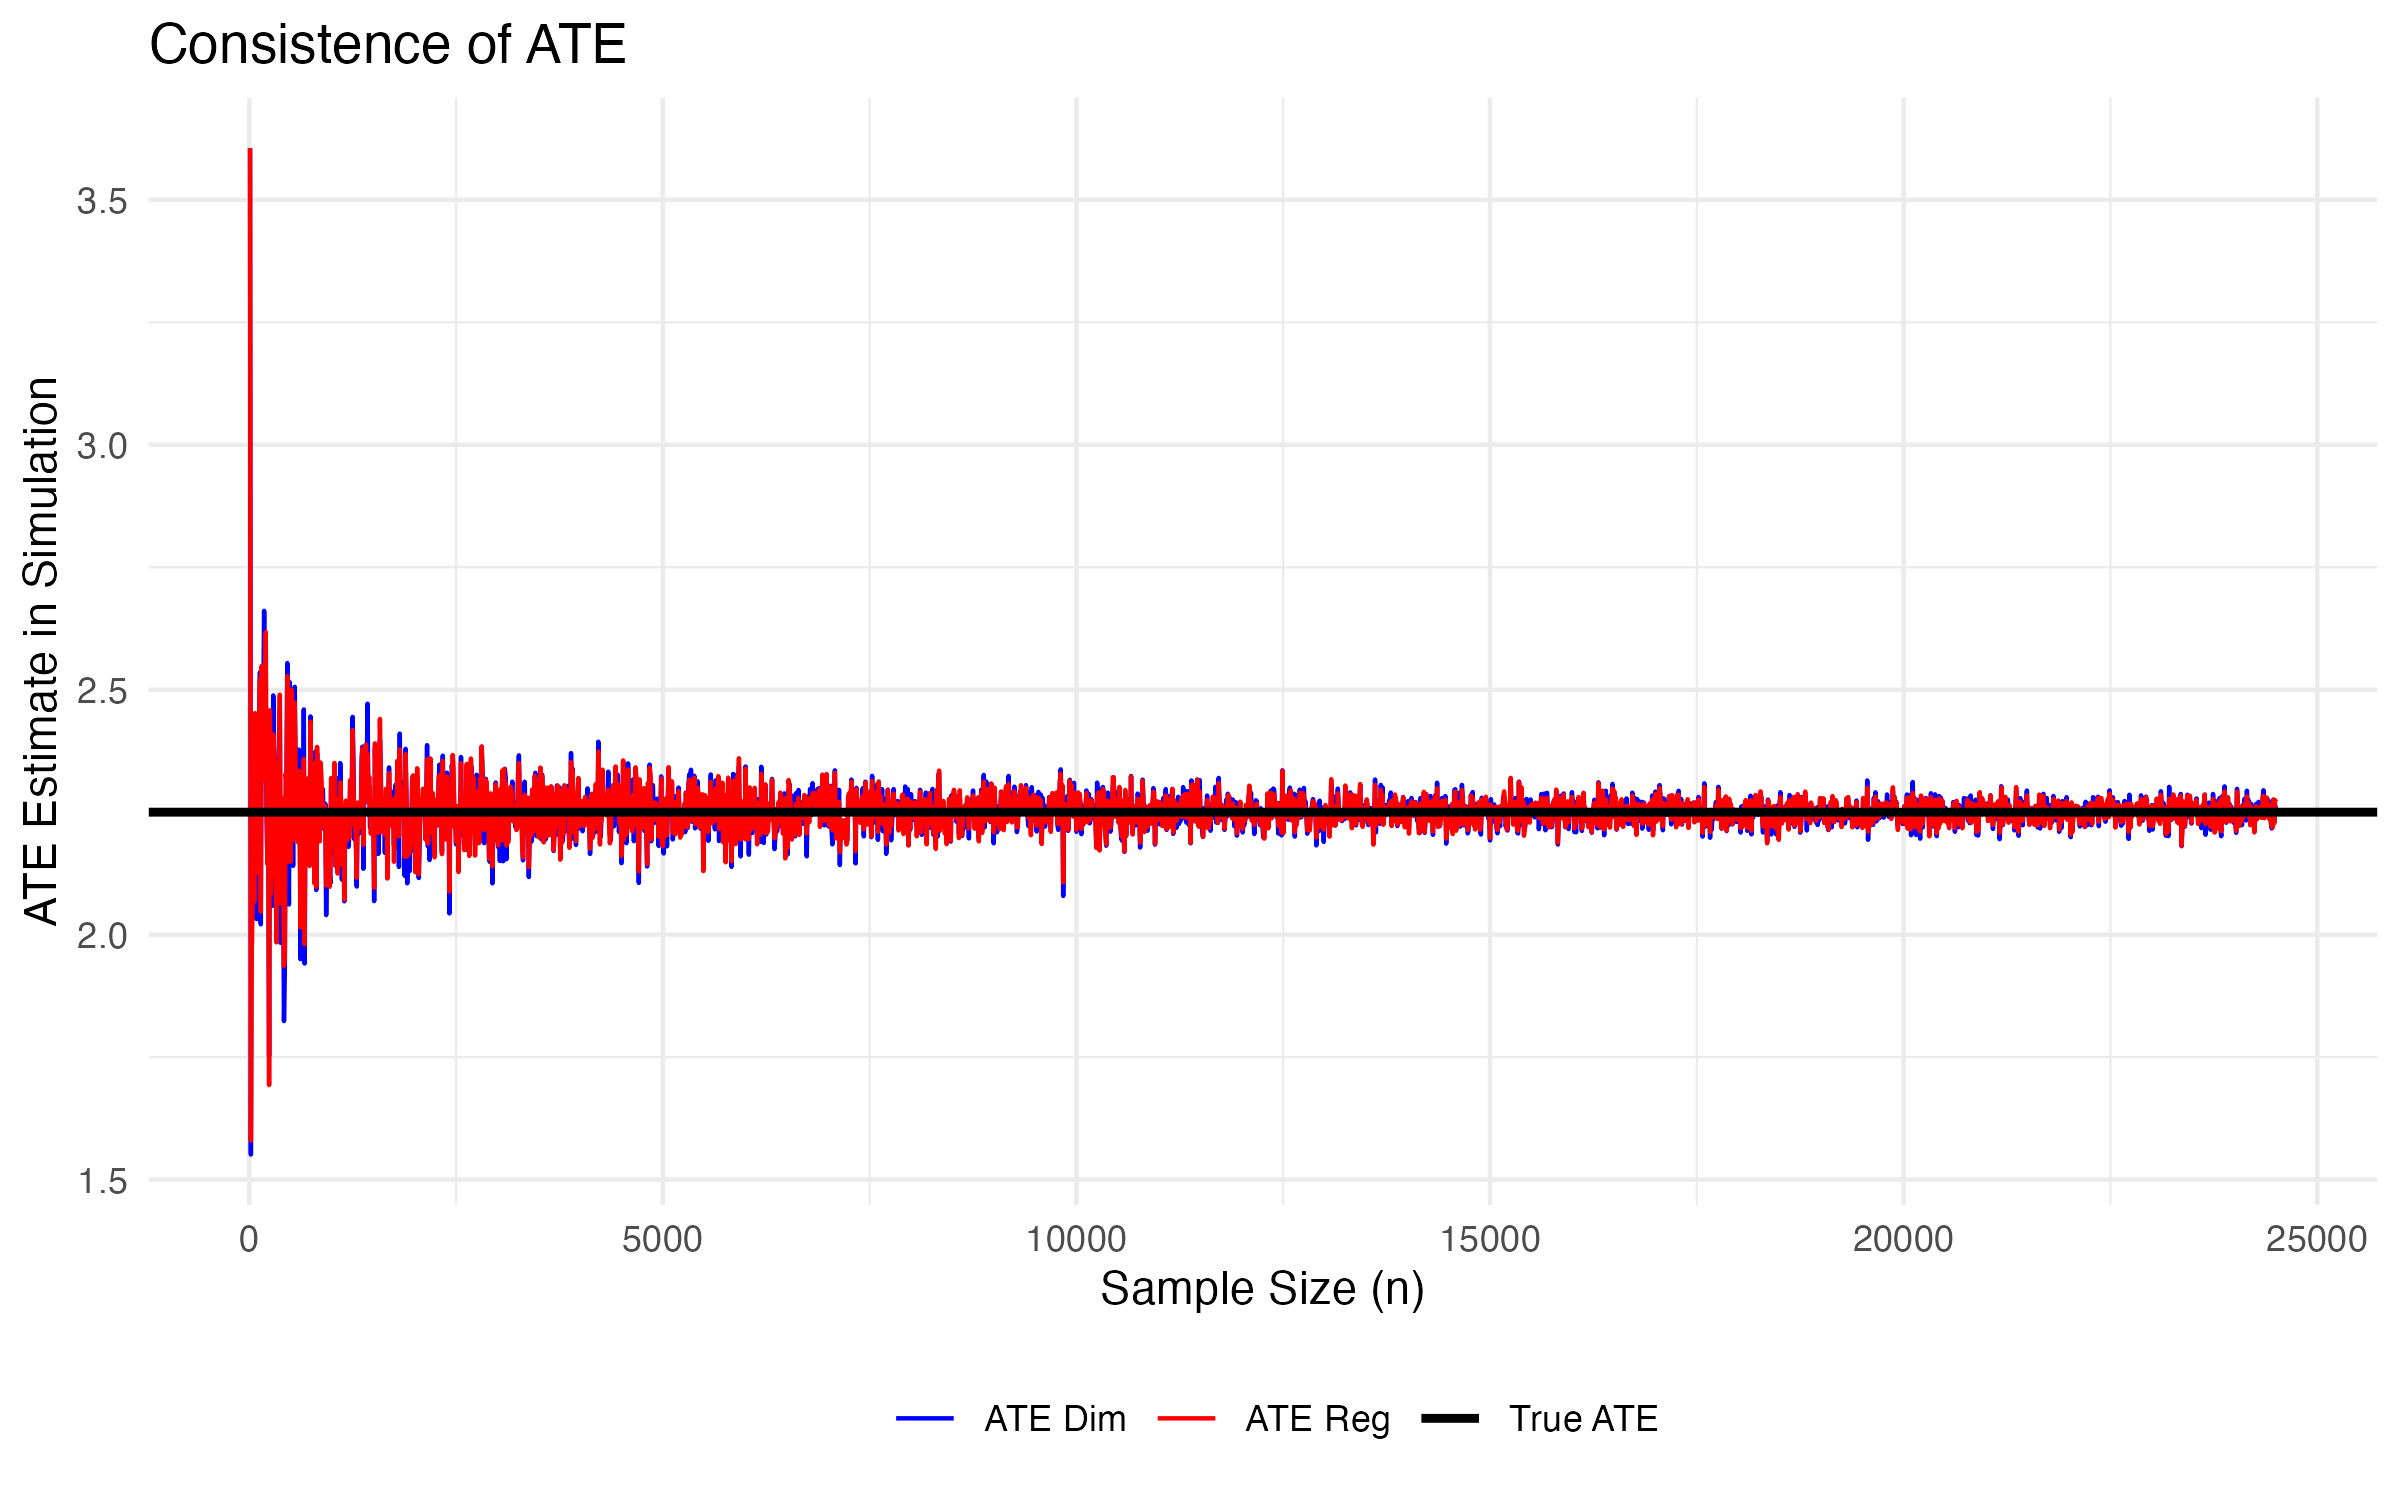
\includegraphics[width=\textwidth]{monte_carlo_ate_consistence.png}
  \caption{Consistency (ATE Estimate vs. Sample Size)}
  \label{fig:your_image_label}
\end{figure}

The simulation agrees with our theoretical conclusion that both estimates are consistents.

\textbf{Conclusion}

Both estimators exhibit negligible bias across all simulation runs, validating their unbiased nature under random treatment assignment and the model specifications.

The Regression-Based Estimator consistently shows lower variance compared to the Difference-in-Means Estimator. This suggests that the regression-based approach is more efficient, providing estimates with less variability across different samples.

Since both estimators are unbiased, the MSE primarily reflects the variance. The regression-based estimator's lower MSE further corroborates its higher efficiency.

This enhanced efficiency of the regression-based approach can be attributed to its utilization of additional information from the covariates and interaction terms. These findings align with theoretical expectations that leveraging a more comprehensive model structure, including interactions and covariates, can yield more efficient estimators in causal inference settings.

Researchers should consider modeling interactions and adjusting for relevant covariates to achieve more reliable and efficient estimates.

\newpage

\begin{colorparagraph}{questioncolor}
\rule{\textwidth}{0.5pt}
\label{q4}\section{Linear Models and Interactions}

We are studying a marketing campaign for a website. We have data from 200 different markets (think of billboards advertising the website placed in different cities) and we observe:
\begin{itemize}
    \item \textbf{visitors} = Total visitors to the website (in hundreds of thousands) coming from that market,
    \item \textbf{spend} = Total spent (in thousands of dollars) on advertising in that market.
\end{itemize}

This data is on Canvas in the file \texttt{marketing\_data.csv}. Assume throughout that changes in spending \textit{cause} changes in visitor numbers. The question is whether the spending on advertising is helping or hurting website traffic and by how much.

We start with the following (heteroskedastic) regression model with independent observations:
\[
visitors_i = \beta_0 + \beta_T \times spend_i + \varepsilon_i, \quad \varepsilon \sim \mathcal{N}(0, \sigma_i^2), \quad \text{correlation}(spend_i, \varepsilon_i) = 0.
\]
\end{colorparagraph}

\begin{colorparagraph}{questioncolor}
\rule{\textwidth}{0.5pt}

\label{q4a}\subsection{Scatter plot and interpretation}
Show a scatter plot of the data along with the fitted regression line from this model. Give a precise and numerical causal interpretation of the results of running this linear regression. How does spending cause visitors to change? Include a discussion of the statistical significance.

\rule{\textwidth}{0.5pt}
\end{colorparagraph}

\begin{figure}[H]
  \centering
  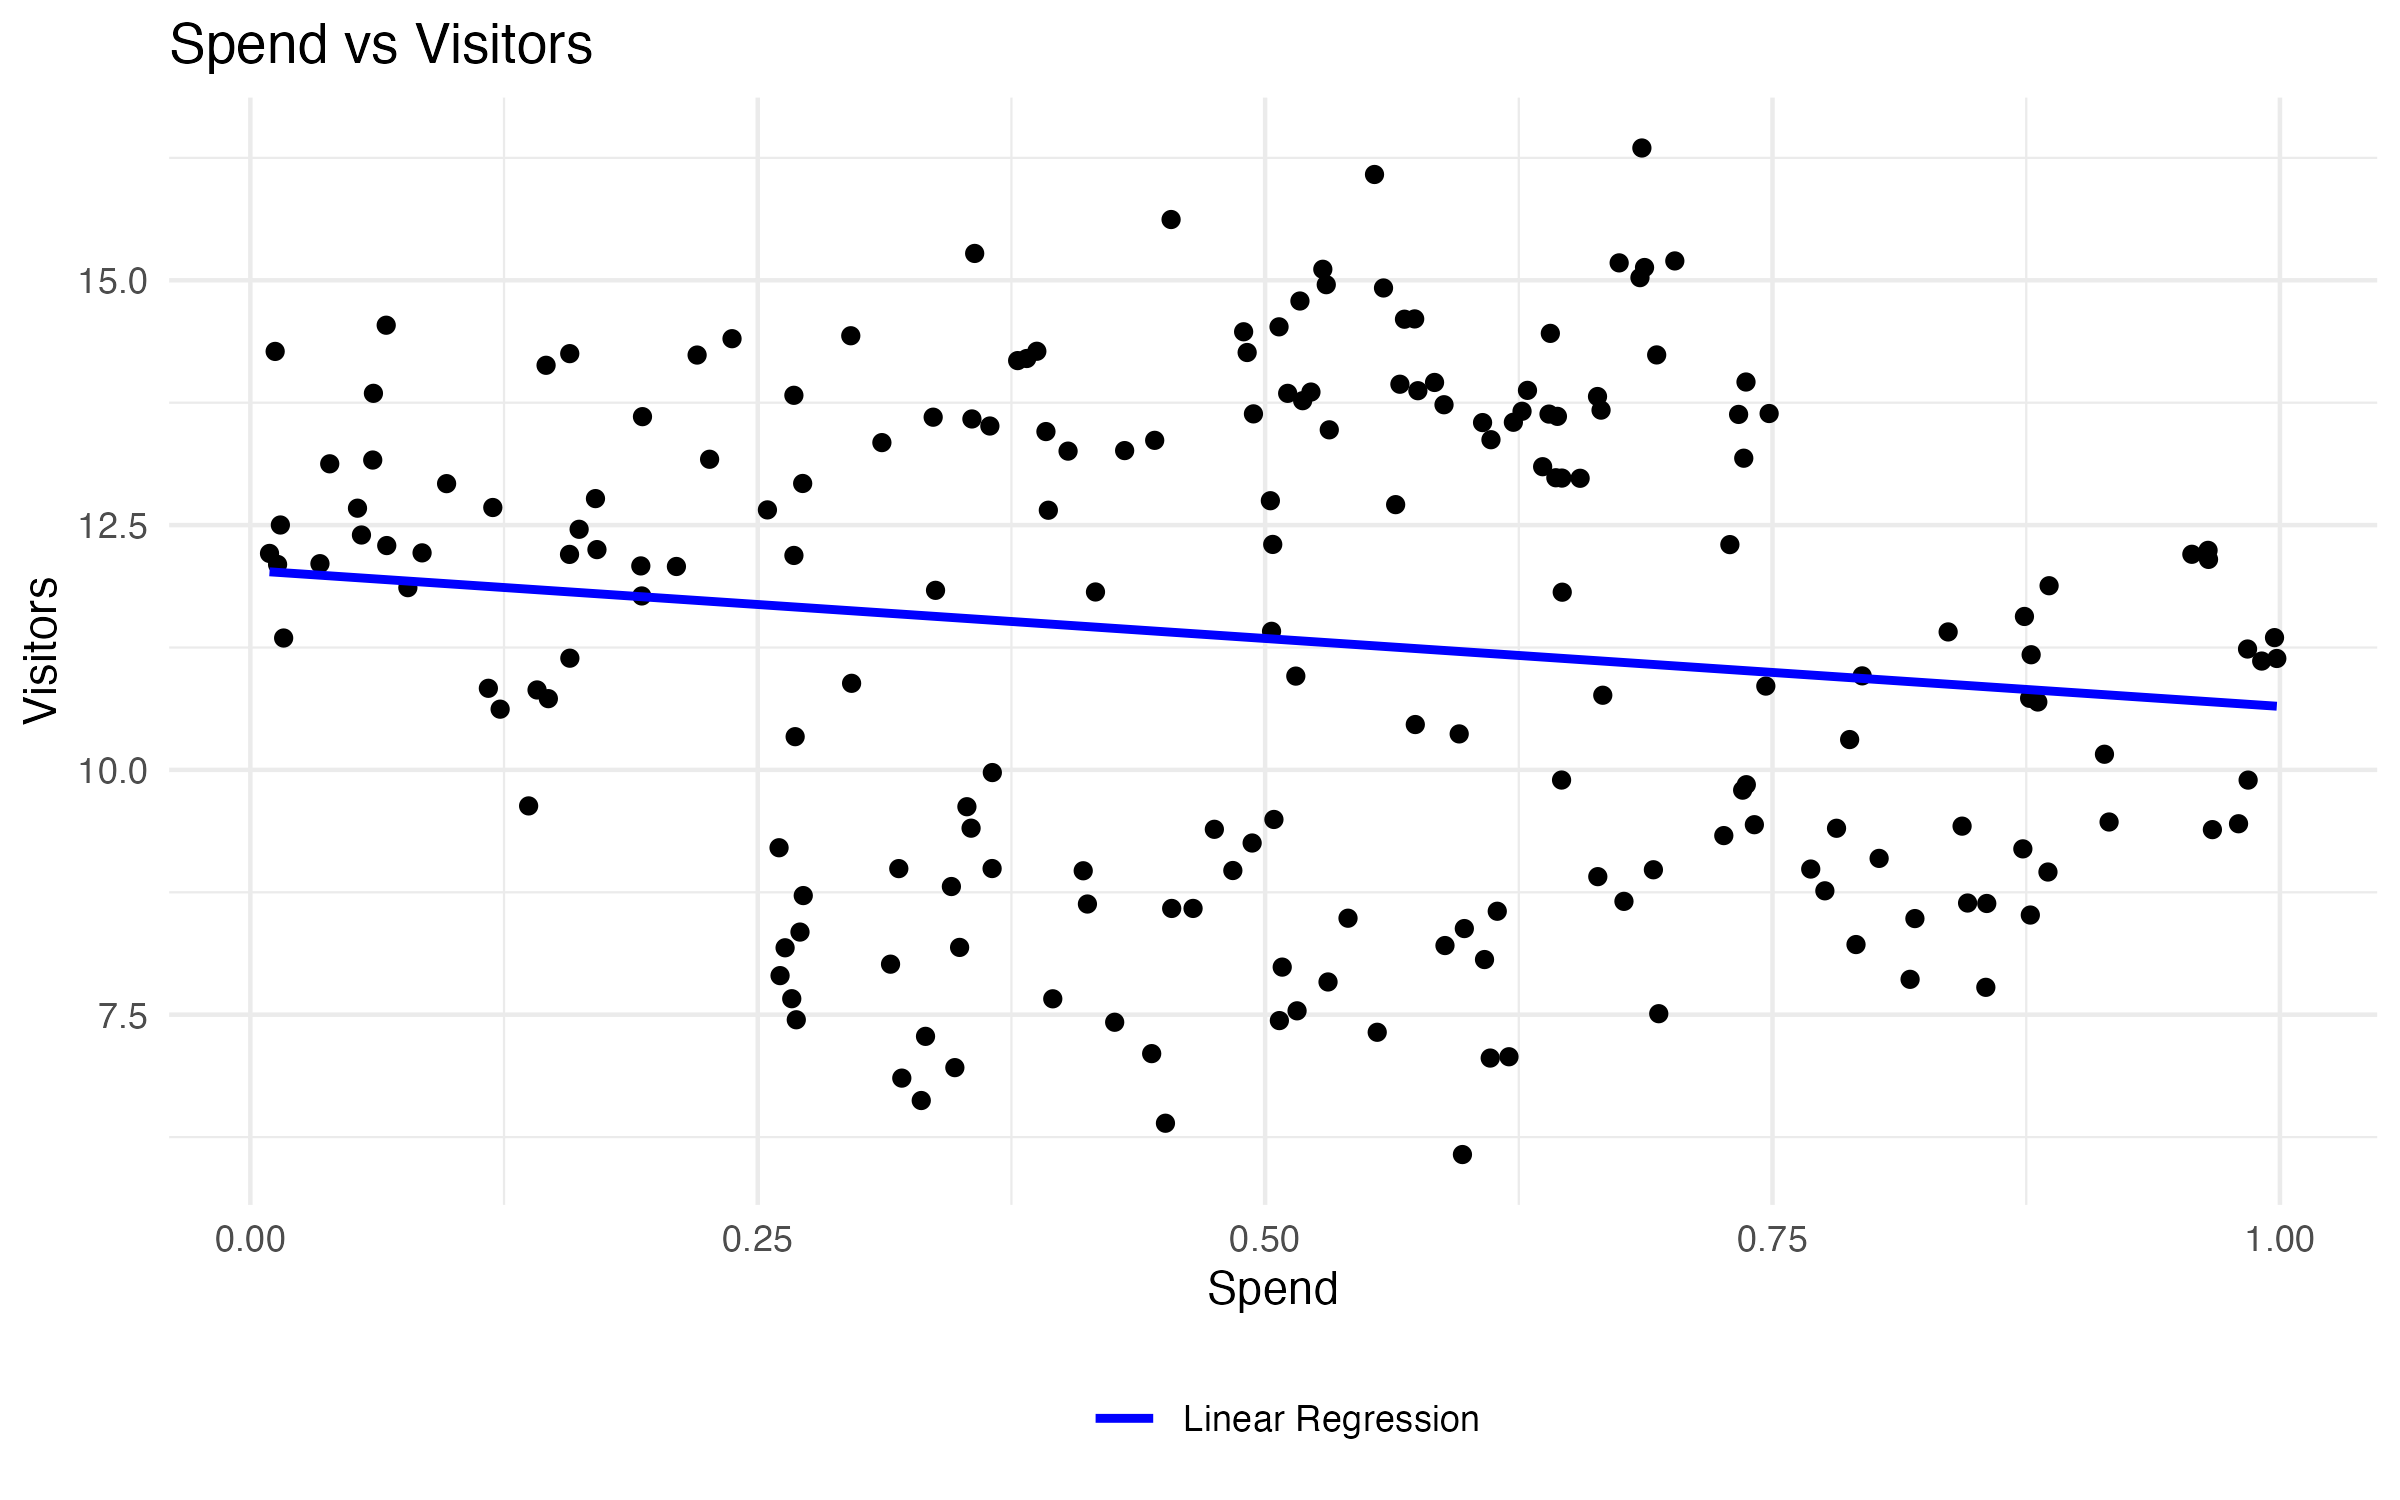
\includegraphics[width=\textwidth]{marketing_spending_vs_visitors.png}
  \caption{Spending vs. Visitors}
  \label{fig:your_image_label}
\end{figure}

The scatter plot illustrates the relationship between advertising spending (\texttt{spend}) and the number of website visitors (\texttt{visitors}) across 200 different markets. The fitted regression line shows the estimated linear relationship derived from the model:
\[
\text{visitors}_i = \beta_0 + \beta_T \times \text{spend}_i + \varepsilon_i
\]

\begin{lstlisting}[style=Rstyle, caption=Linear Model for Visitors]
  library(tidyverse)
  library(readxl)
  
  marketing_data <- read.csv("marketing_data.csv", sep=",") %>% 
    as_tibble() %>% 
    select(-X)
  
  # General Regression and Plot
  ols_visitors_spending <- lm(visitors ~ spend, data = marketing_data)
  summary(ols_visitors_spending)
  
  # Call:
  # lm(formula = visitors ~ spend, data = marketing_data)
  # 
  # Residuals:
  #     Min      1Q  Median      3Q     Max 
  # -5.1353 -2.1523  0.3405  2.1699  5.2667 
  # 
  # Coefficients:
  #             Estimate Std. Error t value Pr(>|t|)    
  # (Intercept)  12.0359     0.3813   31.57   <2e-16 ***
  # spend        -1.3877     0.6768   -2.05   0.0416 *  
  # ---
  # Signif. codes:  0 '***' 0.001 '**' 0.01 \'*\' 0.05 '.' 0.1 ' ' 1
  # 
  # Residual standard error: 2.477 on 198 degrees of freedom
  # Multiple R-squared:  0.02079,	Adjusted R-squared:  0.01585 
  # F-statistic: 4.205 on 1 and 198 DF,  p-value: 0.04163
  
  # By City Regression and Plot
  marketing_data %>% 
    ggplot(aes(x=spend, y=visitors)) +
    geom_point() +
    labs(
      title="Spend vs Visitors",
      x="Spend",
      y="Visitors"
    ) +
    geom_smooth(aes(color = "Linear Regression"), method = "lm", se = FALSE) +
    theme_minimal() +
    scale_color_manual(name = "", values = c("Linear Regression" = "blue")) +
    theme(legend.position = "bottom")
  ggsave("marketing_spending_vs_visitors.png", width = 8, height = 5, dpi = 300)
\end{lstlisting}

From the regression output, the estimated coefficients are:
\[
\begin{aligned}
\hat{\beta}_0 &= 12.0359 \quad (\text{Std. Error: } 0.3813, \; t = 31.57, \; p < 2 \times 10^{-16}) \\
\hat{\beta}_T &= -1.3877 \quad (\text{Std. Error: } 0.6768, \; t = -2.05, \; p = 0.0416)
\end{aligned}
\]

The intercept \(\hat{\beta}_0 = 12.0359\) represents the estimated number of visitors (in hundreds of thousands) when advertising spending is zero. This estimate is statistically significant with a very low p-value (\(p < 2 \times 10^{-16}\)), indicating strong evidence against the null hypothesis that \(\beta_0 = 0\).

The coefficient for \(\texttt{spend}\), \(\hat{\beta}_T = -1.3877\), suggests that for each additional thousand dollars spent on advertising, the number of website visitors decreases by approximately 1.3877 hundred thousand (i.e., 138,770 visitors). The p-value associated with \(\hat{\beta}_T\) is 0.0416, which is below the conventional significance level of 0.05. Therefore, we reject the null hypothesis that \(\beta_T = 0\), concluding that advertising spending has a statistically significant negative effect on website visitors.

Assuming that the model is correctly specified and that all relevant confounders are controlled for, the negative coefficient \(\hat{\beta}_T\) can be interpreted causally. Specifically, increasing advertising spending by one thousand dollars is expected to result in a decrease of approximately 138,770 website visitors, holding all else constant.

Nonetheless, for this causal relationship to hold, assumptions regarding the data generating process and the data must be met. In this scenario we might have:

\begin{enumerate}
  \item Observational data: we should suppose that this is not a randomized experiment. Therefore, it is hard to assume that:
  $$
  Y_i (s) \perp S_i
  $$
  \item Omitted variables: the data generating process can have other features which are not being represented here. If those features are post-treatment, they have influence in the estimated effect of spending on visitors. Even if we had other variables, the causal relationship would only hold if:
  $$
  Y_i (s) \perp S_i | X
  $$
  Meaning that: $\mathbb{E}[Y(s) | S = s, X = x] = \mathbb{E}[Y(s) | X = x]$
  \item Linear model: the data generating process might not be linear, which would state that for different levels of spending the impact on visitors might be different. Even if the model is not linear, if the previous two assumptions hold, we can still recover ATE. Nonetheless, in this last case, assuming linear model when the data generating process would say otherwise does not allow us to recover CATE.
\end{enumerate}

When looking at the presented results above, a researcher should be cautious in stating that those assumptions hold. The small $R^2$ and the scatter plot suggest that collecting data about covariates should help develop a more reliable analysis.

\begin{colorparagraph}{questioncolor}
\rule{\textwidth}{0.5pt}

\label{q4b}\subsection{Increasing visitors}
Using the results above and your answer in (a), if the goal is to increase the visitors to our website, should we raise or lower our spending?

\rule{\textwidth}{0.5pt}
\end{colorparagraph}

If a researcher believes that the previous assumptions hold, the $\beta_T$ represents the ATE. If that is the case, lowering the spending should increase the visitors in the website.

Nonetheless, as stated in the previous answer, one should be cautious to say that the assumptions above hold. The low $R^2$, observational data, possibility of omitted covariates pos-treatment, counterintuitive answer are valid concerns (all stated more clearly in 4.a) that should be considered before making a definitive decision.

\begin{colorparagraph}{questioncolor}
\rule{\textwidth}{0.5pt}

\label{q4c}\subsection{Group Regressions}
Run a linear model of \textit{visitors} on \textit{spend} separately for each group separately. What
do you find and how does this differ from what you found before? In your explanation,
remember that spending causes visitors in this data.

\rule{\textwidth}{0.5pt}
\end{colorparagraph}

\textbf{$\text{city} \in \{0, 1\}$}

We define $\text{city}_i = \text{city}_i - 1$. Therefore, the values that were originally 2 become 1 and the values that were originally 1 become 0. This provides more intuitive results in the following questions.

The analysis of the linear regression models conducted separately for small cities and big cities yields contrasting results compared to the initial regression performed on the entire dataset.

Prior to running the regression, we define $city_i = city_i - 1$, making $city \in \{0, 1\}$, which facilitates further analysis.

\begin{lstlisting}[style=Rstyle, caption=Linear Model for Visitors separeted by City Size]
ols_visitors_spending_small_cities <- lm(
  visitors ~ spend, data = marketing_data_small_cities
)
summary(ols_visitors_spending_small_cities)

# Call:
#   lm(formula = visitors ~ spend, data = marketing_data_small_cities)
# 
# Residuals:
#   Min      1Q  Median      3Q     Max 
# -3.2205 -0.6139 -0.0231  0.8664  2.3934 
# 
# Coefficients:
#   Estimate Std. Error t value Pr(>|t|)    
# (Intercept)  12.2342     0.2196  55.704  < 2e-16 ***
#   spend         2.6232     0.4873   5.383 4.37e-07 ***
#   ---
#   Signif. codes:  0 '***' 0.001 '**' 0.01 '*' 0.05 '.' 0.1 ' ' 1
# 
# Residual standard error: 1.151 on 107 degrees of freedom
# Multiple R-squared:  0.2131,	Adjusted R-squared:  0.2057 
# F-statistic: 28.97 on 1 and 107 DF,  p-value: 4.37e-07


ols_visitors_spending_big_cities <- lm(
  visitors ~ spend, data = marketing_data_big_cities
)
summary(ols_visitors_spending_big_cities)

# Call:
#   lm(formula = visitors ~ spend, data = marketing_data_big_cities)
# 
# Residuals:
#   Min       1Q   Median       3Q      Max 
# -2.84717 -0.85156 -0.05242  0.85707  2.60109 
# 
# Coefficients:
#   Estimate Std. Error t value Pr(>|t|)    
# (Intercept)   6.7741     0.3517  19.259  < 2e-16 ***
#   spend         3.5916     0.5219   6.882 7.95e-10 ***
#   ---
#   Signif. codes:  0 '***' 0.001 '**' 0.01 '*' 0.05 '.' 0.1 ' ' 1
# 
# Residual standard error: 1.153 on 89 degrees of freedom
# Multiple R-squared:  0.3473,	Adjusted R-squared:   0.34 
# F-statistic: 47.37 on 1 and 89 DF,  p-value: 7.952e-10
\end{lstlisting}

\textbf{Regression Results for Small Cities}
$$
\text{visitors}_i = \beta_{0 \text{S}} + \beta_{T \text{S}} \times \text{spend}_i + \varepsilon_i
$$

\[
\begin{aligned}
\text{visitors}_i &= 12.2342 + 2.6232 \times \text{spend}_i + \varepsilon_i, \\
\text{Std. Error} &= [0.2196, \; 0.4873], \\
t\text{-values} &= [55.704, \; 5.383], \\
p\text{-values} &= [<2 \times 10^{-16}, \; 4.37 \times 10^{-07}].
\end{aligned}
\]

\begin{itemize}
  \item The intercept \(\hat{\beta}_0 = 12.2342\) represents the estimated number of visitors (in hundreds of thousands) when advertising spending is zero in small cities. This estimate is highly significant (\(p < 2 \times 10^{-16}\)).
  \item The coefficient for \texttt{spend}, \(\hat{\beta}_{T \text{S}} = 2.6232\), indicates that for each additional thousand dollars spent on advertising in small cities, the number of website visitors increases by approximately 262,320 visitors. This positive relationship is highly statistically significant (\(p = 4.37 \times 10^{-07}\)).
  \item The model explains approximately 21.31\% of the variance in visitor numbers (\(R^2 = 0.2131\)), suggesting a moderate fit.
\end{itemize}

\textbf{Regression Results for Big Cities}
$$
\text{visitors}_i = \beta_{0 \text{B}} + \beta_{T \text{B}} \times \text{spend}_i + \varepsilon_i
$$

\[
\begin{aligned}
\text{visitors}_i &= 6.7741 + 3.5916 \times \text{spend}_i + \varepsilon_i, \\
\text{Std. Error} &= [0.3517, \; 0.5219], \\
t\text{-values} &= [19.259, \; 6.882], \\
p\text{-values} &= [<2 \times 10^{-16}, \; 7.95 \times 10^{-10}].
\end{aligned}
\]

\begin{itemize}
  \item The intercept \(\hat{\beta}_0 = 6.7741\) represents the estimated number of visitors (in hundreds of thousands) when advertising spending is zero in big cities. This estimate is highly significant (\(p < 2 \times 10^{-16}\)).
  \item The coefficient for \texttt{spend}, \(\hat{\beta}_{T \text{B}} = 3.5916\), suggests that for each additional thousand dollars spent on advertising in big cities, the number of website visitors increases by approximately 359,160 visitors. This positive relationship is highly statistically significant (\(p = 7.95 \times 10^{-10}\)).
  \item The model explains approximately 34.73\% of the variance in visitor numbers (\(R^2 = 0.3473\)), indicating a better fit compared to the small cities model.
\end{itemize}

\textbf{Comparison with the Initial Regression}

In the initial regression conducted on the entire dataset, the coefficient for \texttt{spend} was negative (\(\hat{\beta}_T = -1.3877\)) and statistically significant (\(p = 0.0416\)), suggesting that increased advertising spending was associated with a decrease in website visitors, a highly contraintuitive result.

The difference can possibly be explained by:

\begin{itemize}
  \item Omitted variable bias in the aggregate model: the aggregate model does not account for inherent differences between small and big cities. If we assume that the variable city size ($X$) allow us to state that
  $$
  Y_i(s) \perp S_i | X,
  $$
  we can recover the ATE and the regression with the aggregate dataset without considering $X$ does not provide us the ATE.
  \item Lack of interaction term: the initial model does not include interaction term between spending and city size, not allowing for the possibility that the impact on different city sizes are different ($\beta_{T \text{B}} \neq \beta_{T \text{S}}$). Adding an interaction effect can help reconcile the differing effects observed.
  \item Interaction Effects: If big cities generally have higher advertising spending, the positive relationship within big cities might dominate the overall trend. However, if small cities have lower spending with less impact, the aggregation might reflect a complex interplay that results in a negative coefficient.
\end{itemize}

In conclusion, if separating the dataset by city makes $Y_i(s) \perp S_i$, meaning that $\mathbb{E}[Y(s) | S = k] = \mathbb{E}[Y(s)]$ for $s, k \in \Omega$, we can now retrieve the ATE for each kind of city. If that is the case, the causal relationship identified in the previous question is invalid and should be disconsidered. On the other hand, other omitted variables might still exist, not allowing us to do causal inference, even thought we are aware that \texttt{spending} causes \texttt{visitors}.

If this model is well specified, the causal relationship between spending and visitors is positive and the company should hope for an increase in visitors after having increased spending.

\begin{colorparagraph}{questioncolor}
\rule{\textwidth}{0.5pt}

\label{q4d}\subsection{Scatter plot with two regression lines}
Show a scatter plot of the data with these two fitted regression lines, with the different market types shown in different colors.

\rule{\textwidth}{0.5pt}
\end{colorparagraph}

\begin{figure}[H]
  \centering
  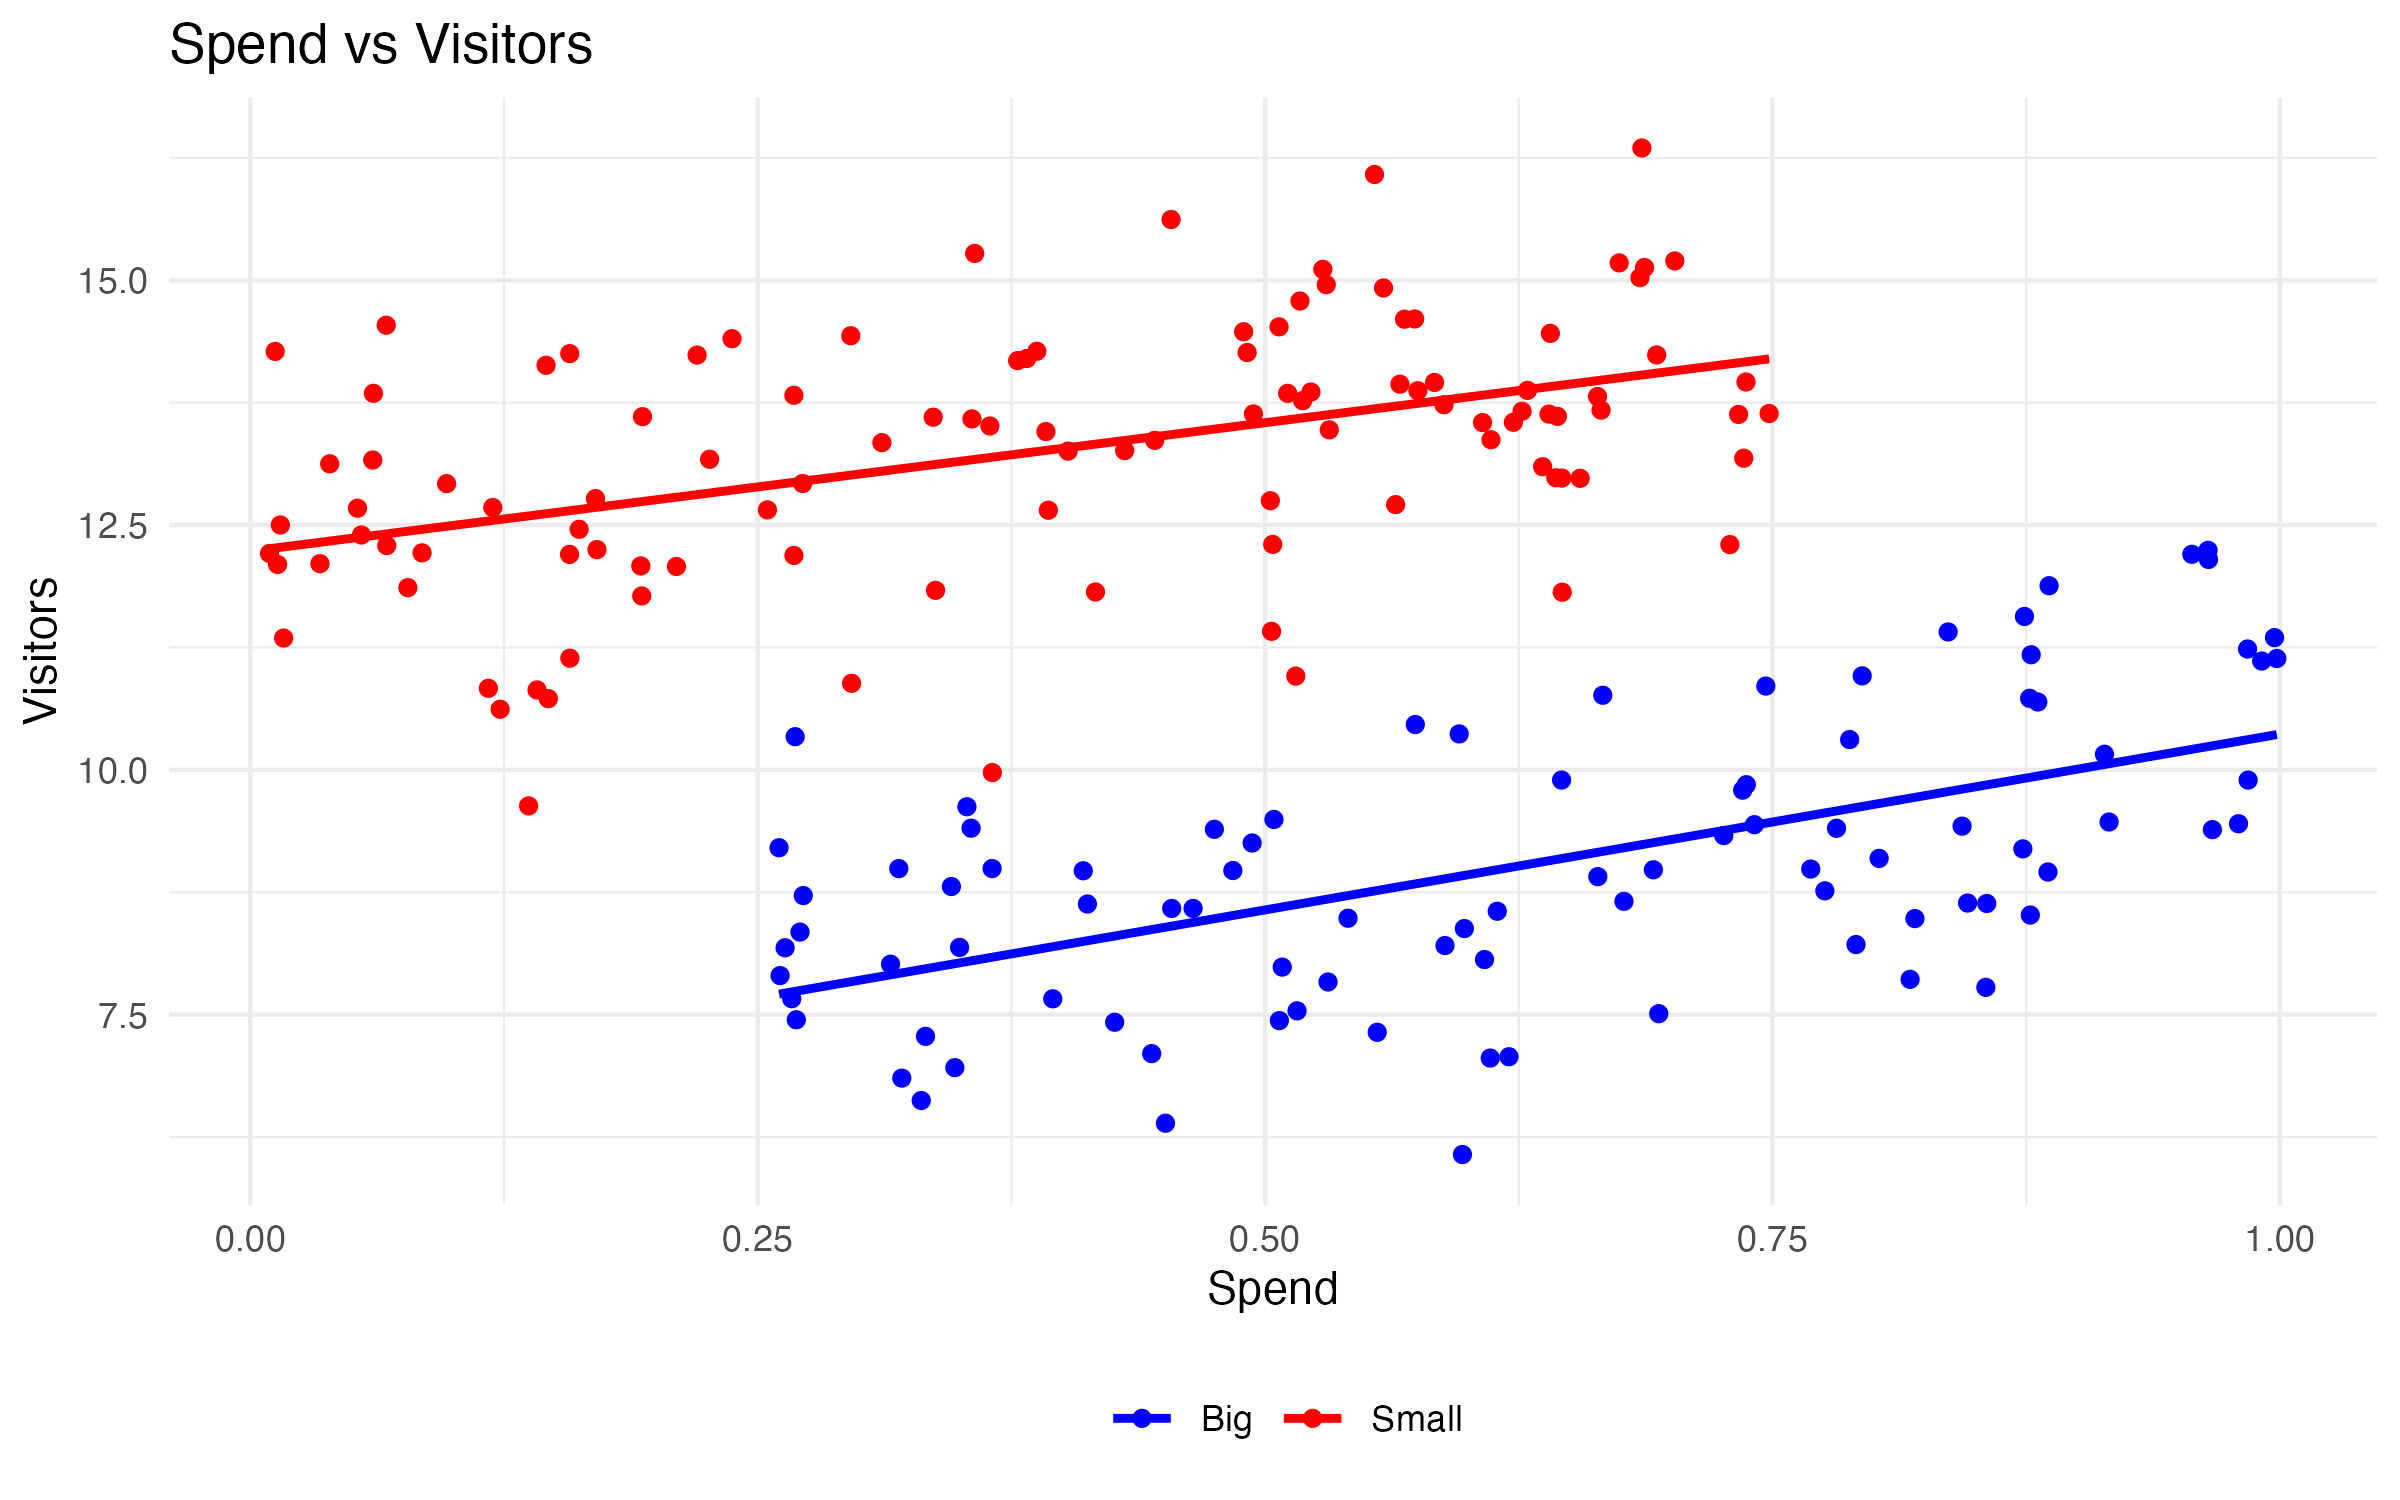
\includegraphics[width=\textwidth]{marketing_spending_vs_visitors_by_city.png}
  \caption{Spending vs. Visitors}
  \label{fig:your_image_label}
\end{figure}

\begin{colorparagraph}{questioncolor}
\rule{\textwidth}{0.5pt}

\label{q4e}\subsection{Single regression with interaction}
Write down a single regression model using \textit{visitors}, \textit{spend}, and \textit{city}, that when taken to the data would yield exactly the four coefficient estimates in part (c). Match up your coefficients to the estimates in (c).

\rule{\textwidth}{0.5pt}
\end{colorparagraph}

\[
\text{visitors}_i = \beta_{0 \text{I}} + \beta_{1 \text{I}} \times \text{spend}_i + \beta_{2 \text{I}} \times \text{city}_i + \beta_{3 \text{I}} \times (\text{spend}_i \times \text{city}_i) + \varepsilon_i
\]

\textbf{$\text{city} \in \{0, 1\}$}

Again, we define $\text{city}_i = \text{city}_i - 1$. Therefore, the values that were originally 2 become 1 and the values that were originally 1 become 0. This provides more intuitive results.

\begin{lstlisting}[style=Rstyle, caption=Linear Model for Visitors separeted by City Size]
# Multivariate Regression
marketing_data_with_interaction <- marketing_data %>%
  mutate(interaction_spend_city = (spend) * city)

ols_visitors_with_interaction <- lm(
  visitors ~ ., data = marketing_data_with_interaction
)
summary(ols_visitors_with_interaction)

# Call:
#   lm(formula = visitors ~ ., data = marketing_data_with_interaction)
# 
# Residuals:
#   Min      1Q  Median      3Q     Max 
# -3.2205 -0.7589 -0.0294  0.8690  2.6011 
# 
# Coefficients:
#   Estimate Std. Error t value Pr(>|t|)    
# (Intercept)             12.2342     0.2199  55.643  < 2e-16 ***
#   spend                    2.6232     0.4879   5.377 2.14e-07 ***
#   city                    -5.4601     0.4144 -13.176  < 2e-16 ***
#   interaction_spend_city   0.9683     0.7139   1.356    0.177    
# ---
#   Signif. codes:  0 '***' 0.001 '**' 0.01 '*' 0.05 '.' 0.1 ' ' 1
# 
# Residual standard error: 1.152 on 196 degrees of freedom
# Multiple R-squared:  0.7903,	Adjusted R-squared:  0.7871 
# F-statistic: 246.2 on 3 and 196 DF,  p-value: < 2.2e-16
\end{lstlisting}

\[
\hat{\text{visitors}}_i = 12.2342 + 2.6232 \times \text{spend}_i - 5.4601 \times \text{city}_i + 0.9684 \times (\text{spend}_i \times \text{city}_i)
\]

\begin{itemize}
  \item \(\hat{\beta}_{0 \text{I}} = 12.2342\): This is the intercept term representing the estimated number of visitors (in hundreds of thousands) when advertising spending is zero and the market is a small city (\(\text{city}_i = 0\)).
  \item \(\hat{\beta}_{1 \text{I}} = 2.6232\): This coefficient represents the effect of advertising spending on visitors in small cities. Specifically, for each additional thousand dollars spent on advertising in a small city, the number of website visitors increases by approximately 262,320.
  \item \(\hat{\beta}_{2 \text{I}} = -5.4601\): This coefficient captures the difference in the intercept between big cities and small cities. It indicates that, holding advertising spending constant, big cities have an estimated 546,010 fewer visitors compared to small cities when advertising spending is zero.
  \item \(\hat{\beta}_{3 \text{I}} = 0.9684\): This interaction term represents the additional effect of advertising spending on visitors in big cities. For each additional thousand dollars spent on advertising in a big city, the number of website visitors increases by approximately 96,840 beyond the effect observed in small cities.
\end{itemize}

\textbf{Matching Coefficients to Group Regressions}

We recover the regression fitted model for small cities is:

$$
\hat{\text{visitors}}_i = 12.2342 + 2.6232 \times \text{spend}_i
$$

And the one for big cities:

$$
\hat{\text{visitors}}_i = 6.7741 + 3.5916 \times \text{spend}_i
$$

The models can be combined into a single model:

$$
\hat{\text{visitors}}_i = c_i (6.7741 + 3.5916 \times \text{spend}_i) + (1 - c_i) (12.2342 + 2.6232 \times \text{spend}_i)
$$

Where $c_i = 1$ if the city is big and $c_i = 0$ if the city is small. The result can be written as:

\begin{align*}
  \hat{\text{visitors}}_i 
  &= c_i (6.7741 + 3.5916 \times \text{spend}_i) + (1 - c_i) (12.2342 + 2.6232 \times \text{spend}_i) \\
  &= c_i (6.7741 + 3.5916 \times \text{spend}_i) + 12.2342 + 2.6232 \times \text{spend}_i - c_i (12.2342 + 2.6232 \times \text{spend}_i) \\
  &=  12.2342 + c_i (6.7741 - 12.2342) + 2.6232 \times \text{spend}_i + c_i (3.5916 \times \text{spend}_i - 2.6232 \times \text{spend}_i) \\
  &=  12.2342 + c_i (6.7741 - 12.2342) + 2.6232 \times \text{spend}_i + c_i \times \text{spend}_i (3.5916 - 2.6232) \\
  &=  12.2342 - 5.4601 c_i + 2.6232 \times \text{spend}_i + 0.9684 c_i \times \text{spend}_i \\
  &=  12.2342 - 5.4601 \times \text{city}_i + 2.6232 \times \text{spend}_i + 0.9684  \times \text{city}_i \times \text{spend}_i \quad \text{(rewriting city)} \\
\end{align*}

The final line is the model in part (4.e).

In other words, we combine the separate models by city into a single model with interaction.

\begin{itemize}
  \item $\beta_{0 \text{I}} = \beta_{0 \text{S}} = 12.2342$
  \item $\beta_{1 \text{I}} = \beta_{1 \text{S}} = 2.6232$
  \item $\beta_{2 \text{I}} = \beta_{0 \text{B}} - \beta_{0 \text{S}} = 6.7741 - 12.2342 = - 5.4601$: represents the difference between the visitors in big and small cities considering zero spending.
  \item $\beta_{3 \text{I}} = \beta_{1 \text{B}} - \beta_{1 \text{S}} = 3.5916 - 2.6232 = 0.9684$: represents the difference between the generated increased of spend in visitors for big and small cities.
\end{itemize}

\text{city $\in \{1, 2\}$}
The solution without modifying the city variable follows the same approach.

\begin{lstlisting}[style=Rstyle, caption=Combined Model without Modifications in City]
# Call:
# lm(formula = visitors ~ ., data = marketing_data_with_interaction)
# 
# Residuals:
#     Min      1Q  Median      3Q     Max 
# -3.2205 -0.7589 -0.0294  0.8690  2.6011 
# 
# Coefficients:
#                        Estimate Std. Error t value Pr(>|t|)    
# (Intercept)             17.6943     0.5628  31.439   <2e-16 ***
# spend                    1.6549     1.1062   1.496    0.136    
# city                    -5.4601     0.4144 -13.176   <2e-16 ***
# interaction_spend_city   0.9683     0.7139   1.356    0.177    
# ---
# Signif. codes:  0 '***' 0.001 '**' 0.01 '*' 0.05 '.' 0.1 ' ' 1
# 
# Residual standard error: 1.152 on 196 degrees of freedom
# Multiple R-squared:  0.7903,	Adjusted R-squared:  0.7871 
# F-statistic: 246.2 on 3 and 196 DF,  p-value: < 2.2e-16
\end{lstlisting}

\[
\hat{\text{visitors}}_i = 17.6943 + 1.6549 \times \text{spend}_i - 5.4601 \times \text{city}_i + 0.9683 \times (\text{spend}_i \times \text{city}_i)
\]

Again, we merge the models separated by city type to get the combined model:

Small cities:

$$
\hat{\text{visitors}}_i = \hat{\beta}_{0, \text{S}} + \hat{\beta}_{1, \text{S}} \times \text{spend}_i
$$

Big cities:

$$
\hat{\text{visitors}}_i = \hat{\beta}_{0, \text{B}} + \hat{\beta}_{1, \text{B}} \times \text{spend}_i
$$

The combined model becomes:

\begin{align*}
\hat{\text{visitors}}_i
=& (2 - \text{city}_i) \left[\hat{\beta}_{0, \text{S}} + \hat{\beta}_{1, \text{S}} \times \text{spend}_i\right]
+ (\text{city}_i - 1)\left[\hat{\beta}_{0, \text{B}} + \hat{\beta}_{1, \text{B}} \times \text{spend}_i\right]
\end{align*}

Which can be viewed as:

\begin{align*}
\hat{\text{visitors}}_i
=& \ (2 - \text{city}_i) \left[\hat{\beta}_{0, \text{S}} + \hat{\beta}_{1, \text{S}} \times \text{spend}_i\right] \quad \text{(becomes 0 when $city_i = 2$ - big)} \\
&+ (\text{city}_i - 1)\left[\hat{\beta}_{0, \text{B}} + \hat{\beta}_{1, \text{B}} \times \text{spend}_i\right] \quad \text{(becomes 0 when $city_i = 1$ - small)}
\end{align*}

The model can be rearranged to:

\begin{align*}
\hat{\text{visitors}}_i
=& \ \left[ 2 \hat{\beta}_{0, \text{S}} - \hat{\beta}_{0, \text{B}} \right] 
     + \left[ 2 \hat{\beta}_{1, \text{S}} - \hat{\beta}_{1, \text{B}} \right] \text{spend}_i \\
     &+ \left[ \hat{\beta}_{0, \text{B}} - \hat{\beta}_{0, \text{S}} \right] \text{city}_i
     + \left[ \hat{\beta}_{1, \text{B}} - \hat{\beta}_{1, \text{S}} \right] \text{city}_i \times \text{spend}_i
\end{align*}

Here, we can rewrite (4.e) as parts of (4.c) again:

$$
2 \hat{\beta}_{0, \text{S}} - \hat{\beta}_{0, \text{B}} = 2 (12.2342) - 6.7741 = 17.6943 = \hat{\beta}_{0, \text{I}}
$$

$$
2 \hat{\beta}_{1, \text{S}} - \hat{\beta}_{1, \text{B}} = 2 (2.6232) - 3.5916 = 1.6742 = \hat{\beta}_{1, \text{I}}
$$

$$
\hat{\beta}_{0, \text{B}} - \hat{\beta}_{0, \text{S}} = 12.2342 - 6.7741 = -5.4601 = \hat{\beta}_{2, \text{I}}
$$

$$
\hat{\beta}_{1, \text{B}} - \hat{\beta}_{1, \text{S}} = 3.5916 - 2.6232 = 0.9614 = \hat{\beta}_{3, \text{I}}
$$



\begin{colorparagraph}{questioncolor}
\rule{\textwidth}{0.5pt}

\label{q4f}\subsection{Expression for \(\beta_T\)}
Give an expression for \(\beta_T\), from the model shown before part (a), in terms of the pieces of your model in part (e) and other features of the relationships between the three observed variables. Assume more things if you need to but be explicit. Use this expression to highlight what features of the data (i.e. the data generating process in the population) are leading to the differences between the separate fits in parts (c) and (e) compared to the combined fit in part (a). Demonstrate these using the data.

\textit{(For future reference, this phenomenon is called "Simpson Paradox")}

\rule{\textwidth}{0.5pt}
\end{colorparagraph}

\textbf{$\text{city} \in \{0, 1\}$}

Again, we define $\text{city}_i = \text{city}_i - 1$. Therefore, the values that were originally 2 become 1 and the values that were originally 1 become 0. This provides more intuitive results.

To express \(\beta_T\) from Model (4.a) in terms of the parameters from the model in (4.e), we begin by considering the definitions of both models.

\textbf{Model 4.a}:

\[
\text{visitors}_i = \beta_0 + \beta_T \times \text{spend}_i + \varepsilon_i,
\]

where \(\beta_T\) represents the average effect of \(\text{spend}_i\) on \(\text{visitors}_i\) across all markets.

\textbf{Model 4.e}:

\[
\text{visitors}_i = \beta_{0 \text{I}} + \beta_{1 \text{I}} \times \text{spend}_i + \beta_{2 \text{I}} \times \text{city}_i + \beta_{3 \text{I}} \times \text{spend}_i \times \text{city}_i + \varepsilon_i.
\]

Our goal is to derive an expression for \(\beta_T\) in terms of \(\beta_{1 \text{I}}\), \(\beta_{2 \text{I}}\), \(\beta_{3 \text{I}}\), and relevant statistical properties of the data.

We start by computing the covariance between \(\text{visitors}_i\) and \(\text{spend}_i\) in Model (4.e):

$$
\mathbb{COV}(\text{visitors}_i, \text{spend}_i)
= \mathbb{COV}(\beta_{0 \text{I}} + \beta_{1 \text{I}} \times \text{spend}_i + \beta_{2 \text{I}} \times \text{city}_i + \beta_{3 \text{I}} \times \text{spend}_i \times \text{city}_i + \varepsilon_i, \, \text{spend}_i)
$$

\begin{align*}
\mathbb{COV}(\text{visitors}_i, \text{spend}_i)
=& \ \beta_{1 \text{I}} \times \mathbb{V}(\text{spend}_i) + \beta_{2 \text{I}} \times \mathbb{COV}(\text{city}_i, \text{spend}_i) \\
&+ \beta_{3 \text{I}} \times \mathbb{COV}(\text{spend}_i \times \text{city}_i, \text{spend}_i) + \mathbb{COV}(\varepsilon_i, \text{spend}_i).
\end{align*}

Since \(\varepsilon_i\) is uncorrelated with \(\text{spend}_i\), \(\mathbb{COV}(\varepsilon_i, \text{spend}_i) = 0\). Therefore:

\[
\mathbb{COV}(\text{visitors}_i, \text{spend}_i) = \beta_{1 \text{I}} \times \mathbb{V}(\text{spend}_i) + \beta_{2 \text{I}} \times \mathbb{COV}(\text{city}_i, \text{spend}_i) + \beta_{3 \text{I}} \times \mathbb{COV}(\text{spend}_i \times \text{city}_i, \text{spend}_i).
\]

In model (4.a), we have:

\[
\beta_T = \frac{\mathbb{COV}(\text{visitors}_i, \text{spend}_i)}{\mathbb{V}(\text{spend}_i)}.
\]

Substituting the expression for \(\mathbb{COV}(\text{visitors}_i, \text{spend}_i)\), we get:

\[
\beta_T = \beta_{1 \text{I}} + \beta_{2 \text{I}} \times \frac{\mathbb{COV}(\text{city}_i, \text{spend}_i)}{\mathbb{V}(\text{spend}_i)} + \beta_{3 \text{I}} \times \frac{\mathbb{COV}(\text{spend}_i \times \text{city}_i, \text{spend}_i)}{\mathbb{V}(\text{spend}_i)}.
\]

Using statistics calculated from data:

\begin{itemize}
    \item \(\beta_{1 \text{I}} = 2.6232\)
    \item \(\beta_{2 \text{I}} = -5.4601\)
    \item \(\beta_{3 \text{I}} = 0.9683\)
    \item \(\mathbb{COV}(\text{city}_i, \text{spend}_i) = 0.06058889\)
    \item \(\mathbb{COV}(\text{spend}_i \times \text{city}_i, \text{spend}_i) = 0.0628975\)
    \item \(\mathbb{V}(\text{spend}_i) = 0.06729443\)
\end{itemize}

Compute the ratios:

\[
\frac{\mathbb{COV}(\text{city}_i, \text{spend}_i)}{\mathbb{V}(\text{spend}_i)} = \frac{0.06058889}{0.06729443} \approx 0.9,
\]

\[
\frac{\mathbb{COV}(\text{spend}_i \times \text{city}_i, \text{spend}_i)}{\mathbb{V}(\text{spend}_i)} = \frac{0.0628975}{0.06729443} \approx 0.935.
\]

Now, calculate \(\beta_T\):

\[
\beta_T = 2.6232 + (-5.4601) \times 0.9 + 0.9683 \times 0.935,
\]

\[
\beta_T = 2.6232 - 4.91409 + 0.906,
\]

\[
\beta_T = (-2.29089) + 0.906 = -1.38489.
\]

Thus, the expression for \(\beta_T\) in terms of the parameters from the model (4.e) is:

\[
\beta_T = \beta_{1 \text{I}} + \beta_{2 \text{I}} \times \frac{\mathbb{COV}(\text{city}_i, \text{spend}_i)}{\mathbb{V}(\text{spend}_i)} + \beta_{3 \text{I}} \times \frac{\mathbb{COV}(\text{spend}_i \times \text{city}_i, \text{spend}_i)}{\mathbb{V}(\text{spend}_i)}.
\]

This result demonstrates how the covariance between \(\text{city}_i\) and \(\text{spend}_i\), as well as the covariance between the interaction term \(\text{spend}_i \times \text{city}_i\) and \(\text{spend}_i\), influence the overall effect of \(\text{spend}_i\) on \(\text{visitors}_i\) in model (4.a).

\textbf{Features of the Data Leading to Differences Between Models}

The differences between the fits in Model E and model (4.a) arise due to the following features of the data:

\begin{itemize}
    \item Correlation between city and spend:
    The covariance \(\mathbb{COV}(\text{city}_i, \text{spend}_i) = 0.06058889\) indicates that advertising spend is higher in big cities (\(\text{city}_i = 1\)) compared to small cities. This positive correlation means that city markets tend to have higher advertising spend.

    \item Interaction effect between spend and city:
    The covariance \(\mathbb{COV}(\text{spend}_i \times \text{city}_i, \text{spend}_i) = 0.0628975\) reflects how the effect of advertising spend on visitors differs between big and small cities. The positive covariance reinforces the interaction between \(\text{spend}_i\) and \(\text{city}_i\) significantly affects the total impact of \(\text{spend}_i\) on \(\text{visitors}_i\).

    \item Variation in spend across cities:
    From the data, the average spend in big cities is higher than in small cities:
    \[
      \hat{\mu}_S: 0.390, \quad \hat{\mu}_B: 0.633.
    \]
    This difference contributes to the covariance terms and thus affects the estimation of \(\beta_T\).

    \item Omission of city effects in model (4.a):
    model (4.a) does not account for the city-specific effects and interactions present in the data. As a result, it provides an average effect that blends the differing relationships in big and small cities, leading to a different estimate of \(\beta_T\).
\end{itemize}

By incorporating the covariances and variances from the data into the expression for \(\beta_T\), we see how the city-related variables influence the overall effect of advertising spend:

\begin{itemize}
    \item The term \(\beta_{2 \text{I}} \times \frac{\mathbb{COV}(\text{city}_i, \text{spend}_i)}{\mathbb{V}(\text{spend}_i)}\) adjusts for the fact that spend is higher in big cities and that big cities have a different baseline number of visitors (captured by \(\beta_{2 \text{I}}\)).

    \item The term \(\beta_{3 \text{I}} \times \frac{\mathbb{COV}(\text{spend}_i \times \text{city}_i, \text{spend}_i)}{\mathbb{V}(\text{spend}_i)}\) captures the differential effect of spend on visitors in big cities versus small cities.

    \item The combined effect shows that, despite \(\beta_{1 \text{I}}\) being positive (2.6232), the overall \(\beta_T\) becomes negative due to the substantial negative adjustment from the city-related terms.
\end{itemize}

In conclusion, this analysis highlights how the differences in advertising spend between big cities and small cities, along with the interaction effects, lead to the differences observed between the separate fits in model (4.a) and the combined fit in model (4.a).

\textbf{Model without modification, city $\in \{1, 2\}$}

If we consider city $\in \{1, 2\}$, the theorical solution is still the same:


\[
\beta_T = \beta_{1 \text{I}} + \beta_{2 \text{I}} \times \frac{\mathbb{COV}(\text{city}_i, \text{spend}_i)}{\mathbb{V}(\text{spend}_i)} + \beta_{3 \text{I}} \times \frac{\mathbb{COV}(\text{spend}_i \times \text{city}_i, \text{spend}_i)}{\mathbb{V}(\text{spend}_i)}.
\]

We only find difference in the data:

\begin{itemize}
    \item \(\beta_{1 \text{I}} = 1.6549\)
    \item \(\beta_{2 \text{I}} = -5.4601\)
    \item \(\beta_{3 \text{I}} = 0.9683\)
    \item \(\mathbb{COV}(\text{city}_i, \text{spend}_i) = 0.06058889\)
    \item \(\mathbb{COV}(\text{spend}_i \times \text{city}_i, \text{spend}_i) = 0.1301919\)
    \item \(\mathbb{V}(\text{spend}_i) = 0.06729443\)
\end{itemize}

The modifications occur in $\beta_{1 \text{I}}$ and $\mathbb{COV}(\text{spend}_i \times \text{city}_i, \text{spend}_i)$.

\[
\beta_T = \beta_{1 \text{I}} + \beta_{2 \text{I}} \times \frac{\mathbb{COV}(\text{city}_i, \text{spend}_i)}{\mathbb{V}(\text{spend}_i)} + \beta_{3 \text{I}} \times \frac{\mathbb{COV}(\text{spend}_i \times \text{city}_i, \text{spend}_i)}{\mathbb{V}(\text{spend}_i)}.
\]

Compute the new ratios:

\[
\frac{\mathbb{COV}(\text{city}_i, \text{spend}_i)}{\mathbb{V}(\text{spend}_i)} = \frac{0.06058889}{0.06729443} \approx 0.9,
\]

\[
\frac{\mathbb{COV}(\text{spend}_i \times \text{city}_i, \text{spend}_i)}{\mathbb{V}(\text{spend}_i)} = \frac{0.1301919}{0.06729443} \approx 1.935.
\]

\[
\beta_T = 1.6549 + (-5.4601) \times 0.9 + 0.9683 \times 1.935 = -1.385529
\]

Successfully, the result again matches.

% \begin{colorparagraph}{questioncolor}
% \section*{Questions 2.f to 2.l with $\bar{x}_i$}
% \end{colorparagraph}

% \begin{colorparagraph}{questioncolor}
% \label{qe2f}\subsection*{2.f \quad Least squares on demeaned covariates}
% First, we run least squares on demeaned covariates separately in each group to obtain \(\hat{\theta}_t = (\hat{\alpha}_t, \hat{\beta}_t)'\) as
% \[
% (\hat{\alpha}_t, \hat{\beta}_t) = \arg\min_{a,b} \sum_{i=1}^{n} 1\{t_i = t\} \left( y_i - a - b(x_i - \bar{x}_t) \right)^2.
% \]
% Give closed form solutions for the vector \(\hat{\theta}_t = (\hat{\alpha}_t, \hat{\beta}_t)'\) using matrix notation and give conditions for the solutions to exist and be unique.
% \end{colorparagraph}

% \textbf{Treatment Group $t = 1$}

% When $t = 1$ we sum only over $n_1$:

% \[
% (\hat{\alpha}_1, \hat{\beta}_1) = \arg\min_{a,b} \sum_{j=1}^{n_1} \left( y_j - a - b(x_j - \bar{x}_1) \right)^2.
% \]

% $Y$ is $n_1 \times 1$ and $X$ is $n_1 \times 2$:

% $$
% Y_1 = \left[
%   \begin{matrix}
%   y_1 \\
%   y_2 \\
%   y_3 \\
%   \vdots \\
%   y_{n_1} \\
%   \end{matrix}
% \right], \quad
% X_1 = \left[
% \begin{matrix}
%   1 & (x_1 - \bar{x}_1) \\
%   1 & (x_2 - \bar{x}_1) \\
%   1 & (x_3 - \bar{x}_1) \\ 
%   \vdots & \vdots \\ 
%   1 & (x_{n_1} - \bar{x}_1) \\ 
% \end{matrix}
% \right]
% $$

% Where $\bar{x}_1 = \frac{1}{n_1} \sum_{j = 1}^{n_1} x_j = \frac{1}{n_1} \sum_{i = 1}^{n} x_i t_i$

% Following the derivation of 2.c,

% $$
% (\hat{\alpha}_1, \hat{\beta}_1) = (X_1'X_1)^{-1} X_1' Y_1
% $$

% Where:


% \begin{align*}
%   X_1'X_1  
%   &= \left[
%     \begin{matrix}
%       n_1 & \sum_{j = 1}^{n_1} (x_j - \bar{x}_1) \\
%       \sum_{j = 1}^{n_1} (x_j - \bar{x}_1) & \sum_{j = 1}^{n_1} (x_j - \bar{x}_1)^2 \\
%     \end{matrix}
%   \right] \\
%   &= \left[
%     \begin{matrix}
%       n_1 & 0 \\
%       0 & \sum_{j = 1}^{n_1} (x_j - \bar{x}_1)^2 \\
%     \end{matrix}
%   \right] \\
%   &= \left[
%     \begin{matrix}
%       n_1 & 0 \\
%       0 & \mathbb{V}[x_j | t = 1] \\
%     \end{matrix}
%   \right] \\
%   &= \left[
%     \begin{matrix}
%       n_1 & 0 \\
%       0 & \sigma_{x, 1}^2 \\
%     \end{matrix}
%   \right] \\
% \end{align*}

% The simplication $\sum_{j = 1}^{n_1} (x_j - \bar{x}_1) = 0$ can be done because the covariate is demeaned.

% \begin{align*}
%   (X_1'X_1)^{-1}  
%   &= \left[
%     \begin{matrix}
%       n_1 & 0 \\
%       0 & \sigma_{x, 1}^2 \\
%     \end{matrix}
%   \right]^{-1} \\
%   &= \frac{1}{\text{det}(X_1'X_1)} \left[
%     \begin{matrix}
%       \sigma_{x, 1}^2 & 0 \\
%       0 & n_1 \\
%     \end{matrix}
%   \right] \\
%   &= \frac{1}{n_1 \sigma_{x, 1}^2} \left[
%     \begin{matrix}
%       \sigma_{x, 1}^2 & 0 \\
%       0 & n_1 \\
%     \end{matrix}
%   \right] \\
%   &= \left[
%     \begin{matrix}
%       \frac{1}{n_1} & 0 \\
%       0 & \frac{1}{\sigma_{x, 1}^2} \\
%     \end{matrix}
%   \right] \\
% \end{align*}

% $$
% (X_1'X_1)^{-1} X_1^T = \left[
%   \begin{matrix}
%     \frac{1}{n_1} & \frac{1}{n_1} & \hdots & \frac{1}{n_1} \\
%     \frac{x_1 - \bar{x}_1}{\sigma_{x, 1}^2} &
%     \frac{x_2 - \bar{x}_1}{\sigma_{x, 1}^2} &
%     \hdots &
%     \frac{x_{n_1} - \bar{x}_1}{\sigma_{x, 1}^2}
%     \\
%   \end{matrix}
% \right]
% $$

% \begin{align*}
%   (X_1'X_1)^{-1} X_1^T Y_1 
%   &= \left[
%     \begin{matrix}
%       \frac{1}{n_1} & \frac{1}{n_1} & \hdots & \frac{1}{n_1} \\
%       \frac{x_1 - \bar{x}_1}{\sigma_{x, 1}^2} &
%       \frac{x_2 - \bar{x}_1}{\sigma_{x, 1}^2} &
%       \hdots &
%       \frac{x_{n_1} - \bar{x}_1}{\sigma_{x, 1}^2}
%       \\
%     \end{matrix}
%   \right]
%   \left[
%     \begin{matrix}
%       y_1 \\ y_2 \\ \vdots \\ y_{n_1}
%     \end{matrix}
%   \right] \\
%   &= \left[
%     \begin{matrix}
%       \dfrac{1}{n_1} \sum_{j = 1}^{n_1} y_j \\
%       \dfrac{\sum_{j = 1}^{n_1} y_j (x_j - \bar{x}_1)}{\sigma_{x, 1}^2} \\
%     \end{matrix}
%   \right] \\
%   &= \left[
%     \begin{matrix}
%       \dfrac{1}{n_1} \sum_{j = 1}^{n_1} y_j \\
%       \dfrac{\sum_{j = 1}^{n_1} y_j (x_j - \bar{x}_1)}{\sum_{j = 1}^{n_1} (x_j - \bar{x}_1)^2} \\
%     \end{matrix}
%   \right] \\
%   &= \left[
%     \begin{matrix}
%       \hat{\alpha}_1 \\
%       \hat{\beta}_1
%     \end{matrix}
%   \right]
% \end{align*}

% $$
% \hat{\alpha}_1 = \frac{1}{n_1} \sum_{j = 1}^{n_1} y_j, \quad
% \hat{\beta}_1 = \dfrac{\sum_{j = 1}^{n_1} y_j (x_j - \bar{x}_1)}{\sum_{j = 1}^{n_1} (x_j - \bar{x}_1)^2}
% $$

% In order for the solution to exist and be unique, $(X_1'X_1)^{-1}$ must exist, which only can happen when the covariate assumes both values 0 and 1 inside the treatment group.

% If that is not the case, $X_1'X_1$ becomes:

% $$
% \left[
%   \begin{matrix}
%     n_1 & 0 \\
%     0 & 0
%   \end{matrix}
% \right],
% $$

% which is a singular matrix with $\det(X_1'X_1) = 0$. In other words $\bar{x}_1 \neq 0 \cup \bar{x}_1 \neq 1$ for the solution to exist and be unique (which implies $n_1 \geq 2$).

% \textbf{Control Group $t = 0$}

% When $t = 0$ we sum only over $n_0$:

% \[
% (\hat{\alpha}_0, \hat{\beta}_0) = \arg\min_{a,b} \sum_{k=1}^{n_0} \left( y_j - a - b(x_k - \bar{x}_0) \right)^2.
% \]

% $Y_0$ is $n_1 \times 1$ and $X_0$ is $n_0 \times 2$:

% $$
% Y_0 = \left[
%   \begin{matrix}
%   y_1 \\
%   y_2 \\
%   y_3 \\
%   \vdots \\
%   y_{n_0} \\
%   \end{matrix}
% \right], \quad
% X_0 = \left[
% \begin{matrix}
%   1 & (x_1 - \bar{x}_0) \\
%   1 & (x_2 - \bar{x}_0) \\
%   1 & (x_3 - \bar{x}_0) \\ 
%   \vdots & \vdots \\ 
%   1 & (x_{n_0} - \bar{x}_0) \\ 
% \end{matrix}
% \right]
% $$

% Where $\bar{x}_0 = \frac{1}{n_0} \sum_{k = 1}^{n_0} x_k = \frac{1}{n_0} \sum_{i = 1}^{n} x_j (1 - t_j)$

% Following the derivation of 2.c,

% $$
% (\hat{\alpha}_0, \hat{\beta}_0) = (X_0'X_0)^{-1} X_0' Y_0
% $$

% Where:

% \begin{align*}
%   X_0'X_0  
%   &= \left[
%     \begin{matrix}
%       n_0 & \sum_{k = 1}^{n_0} (x_k - \bar{x}_0) \\
%       \sum_{k = 1}^{n_0} (x_k - \bar{x}_0) & \sum_{k = 1}^{n_0} (x_k - \bar{x}_0)^2 \\
%     \end{matrix}
%   \right] \\
%   &= \left[
%     \begin{matrix}
%       n_0 & 0 \\
%       0 & \sum_{k = 1}^{n_0} (x_k - \bar{x}_0)^2 \\
%     \end{matrix}
%   \right] \\
%   &= \left[
%     \begin{matrix}
%       n_0 & 0 \\
%       0 & \mathbb{V}[x_k | t = 0] \\
%     \end{matrix}
%   \right] \\
%   &= \left[
%     \begin{matrix}
%       n_0 & 0 \\
%       0 & \sigma_{x, 0}^2 \\
%     \end{matrix}
%   \right] \\
% \end{align*}

% The simplication $\sum_{k = 1}^{n_0} (x_k - \bar{x}_0) = 0$ can be done because the covariate is demeaned.

% \begin{align*}
%   (X_0'X_0)^{-1}  
%   &= \left[
%     \begin{matrix}
%       n_0 & 0 \\
%       0 & \sigma_{x, 0}^2 \\
%     \end{matrix}
%   \right]^{-1} \\
%   &= \frac{1}{\text{det}(X_0'X_0)} \left[
%     \begin{matrix}
%       \sigma_{x, 0}^2 & 0 \\
%       0 & n_0 \\
%     \end{matrix}
%   \right] \\
%   &= \frac{1}{n_0 \sigma_{x, 0}^2} \left[
%     \begin{matrix}
%       \sigma_{x, 0}^2 & 0 \\
%       0 & n_0 \\
%     \end{matrix}
%   \right] \\
%   &= \left[
%     \begin{matrix}
%       \frac{1}{n_0} & 0 \\
%       0 & \frac{1}{\sigma_{x, 0}^2} \\
%     \end{matrix}
%   \right] \\
% \end{align*}

% $$
% (X_0'X_0)^{-1} X_0^T = \left[
%   \begin{matrix}
%     \frac{1}{n_0} & \frac{1}{n_0} & \hdots & \frac{1}{n_0} \\
%     \frac{x_1 - \bar{x}_0}{\sigma_{x, 0}^2} &
%     \frac{x_2 - \bar{x}_0}{\sigma_{x, 0}^2} &
%     \hdots &
%     \frac{x_{n_0} - \bar{x}_0}{\sigma_{x, 0}^2}
%     \\
%   \end{matrix}
% \right]
% $$

% \begin{align*}
%   (X_0'X_0)^{-1} X_0^T Y_0 
%   &= \left[
%     \begin{matrix}
%       \frac{1}{n_0} & \frac{1}{n_0} & \hdots & \frac{1}{n_0} \\
%       \frac{x_1 - \bar{x}_0}{\sigma_{x, 0}^2} &
%       \frac{x_2 - \bar{x}_0}{\sigma_{x, 0}^2} &
%       \hdots &
%       \frac{x_{n_0} - \bar{x}_0}{\sigma_{x, 0}^2}
%       \\
%     \end{matrix}
%   \right]
%   \left[
%     \begin{matrix}
%       y_1 \\ y_2 \\ \vdots \\ y_{n_0}
%     \end{matrix}
%   \right] \\
%   &= \left[
%     \begin{matrix}
%       \dfrac{1}{n_0} \sum_{k = 1}^{n_0} y_k \\
%       \dfrac{\sum_{k = 1}^{n_0} y_k (x_k - \bar{x}_0)}{\sigma_{x, 0}^2} \\
%     \end{matrix}
%   \right] \\
%   &= \left[
%     \begin{matrix}
%       \dfrac{1}{n_0} \sum_{k = 1}^{n_0} y_k \\
%       \dfrac{\sum_{k = 1}^{n_0} y_k (x_k - \bar{x}_0)}{\sum_{k = 1}^{n_0} (x_k - \bar{x}_0)^2} \\
%     \end{matrix}
%   \right] \\
%   &= \left[
%     \begin{matrix}
%       \hat{\alpha}_0 \\
%       \hat{\beta}_0
%     \end{matrix}
%   \right]
% \end{align*}

% $$
% \hat{\alpha}_0 = \dfrac{1}{n_0} \sum_{k = 1}^{n_0} y_k, \quad
% \hat{\beta}_0 = \dfrac{\sum_{k = 1}^{n_0} y_k (x_k - \bar{x}_0)}{\sum_{k = 1}^{n_0} (x_k - \bar{x}_0)^2}
% $$

% In order for the solution to exist and be unique, $(X_0'X_0)^{-1}$ must exist, which only can happen when the covariate assumes both values 0 and 1 inside the control group.

% If that is not the case, $X_0'X_0$ becomes:

% $$
% \left[
%   \begin{matrix}
%     n_0 & 0 \\
%     0 & 0
%   \end{matrix}
% \right],
% $$

% which is a singular matrix with $\det(X_0'X_0) = 0$. In other words $\bar{x}_0 \neq 0 \cup \bar{x}_0 \neq 1$ for the solution to exist and be unique (which implies $n_0 \geq 2$).

% \begin{colorparagraph}{tacolor}QUESTION:
%   Need to ask question to check if it is correct
% \end{colorparagraph}

% \begin{colorparagraph}{questioncolor}
% \label{qe2g}\subsection*{2.g \quad Predicted values for counterfactuals}
% Given \(\hat{\theta}_0\) and \(\hat{\theta}_1\), form predicted values for each potential outcome, i.e., give expressions for \(\hat{Y}_i(1)\) and \(\hat{Y}_i(0)\). Combine these counterfactual predictions with each observation's factual (observed) outcome to obtain estimates of the individual causal effect \(\tau_i = Y_i(1) - Y_i(0)\). Denote these predicted values as \(\hat{\tau}_i\).
% \end{colorparagraph}

% Given the stated assumptions:

% $$
% \mathbb{E}[y_i | t = 1] = \hat{Y}_i (1)
% $$

% $$
% \mathbb{E}[y_i | t = 0] = \hat{Y}_i (0)
% $$

% Furthermore, from the previous derived models:

% $$
% \hat{y}_i = \hat{\alpha}_0 + \hat{\beta}_0 (x_i - \bar{x}_0) \quad \text{when} \ t = 0
% $$

% $$
% \hat{y}_i = \hat{\alpha}_1 + \hat{\beta}_1 (x_i - \bar{x}_1) \quad \text{when} \ t = 1
% $$

% Which can incorporated in a single model:

% \begin{align*}
%   \hat{y}_i &= t_i \left[\hat{\alpha}_1 + \hat{\beta}_1 (x_i - \bar{x}_1)\right]
%             + (1 - t_i) \left[\hat{\alpha}_0 + \hat{\beta}_0 (x_i - \bar{x}_0)\right] \\
%             &= t_i (\hat{\alpha}_1 - \hat{\alpha}_0) + \hat{\alpha}_0 + t_i \left(\hat{\beta}_1 (x_i - \bar{x}_1) - \hat{\beta}_0 (x_i - \bar{x}_1)\right) + \hat{\beta}_0 (x_i - \bar{x}_1)
% \end{align*}

% By definition, conditional to the assumptions of the exercise:

% $$
% \hat{\tau}_i = Y_i(1) - Y_i(0)
% $$

% \begin{align*}
%   \hat{\tau}_i &= (\hat{\alpha}_1 - \hat{\alpha}_0) + \left[\hat{\beta}_1 (x_i - \bar{x}_1) - \hat{\beta}_0 (x_i - \bar{x}_1) \right] \\
%               &= (\hat{\alpha}_1 - \hat{\alpha}_0) + \left[x_i \left(\hat{\beta}_1 - \hat{\beta}_0\right) - \left(\bar{x}_1 - \bar{x}_0\right) \right] \\ 
% \end{align*}

% The predicted value of $\hat{\tau}$ lies in the difference between the intercepts, difference between the slopes of $Y$ with respect to the covariate, and the difference between the average covariate level for each subgroup.

% \begin{colorparagraph}{tacolor}QUESTION:
%   Need to check if the answer is right.
% \end{colorparagraph}

% \begin{colorparagraph}{questioncolor}
% \label{qe2h}\subsection*{2.h \quad Sample average treatment effect}
% Show that \(\hat{\tau}_{\text{pi}} = \frac{1}{n} \sum_{i=1}^{n} \hat{\tau}_i = \hat{\alpha}_1 - \hat{\alpha}_0\), the latter being the intercepts from (2).
% \end{colorparagraph}

% The model to predict observation in which $T = 1$ is:

% \begin{align*}
%   \hat{y}_{i, 1} &= \hat{\alpha}_1 + \hat{\beta}_1 (x_i - \bar{x}_1) \\
%            &= \frac{\sum_{i = 1}^{n_1} y_i}{n_1} + \sum_{i = 1}^{n_1} \frac{ y_i (x_i - \bar{x}_1)}{(x_i - \bar{x}_1)^2} (x_i - \bar{x}_1)\\
% \end{align*}

% And the model to predict observations in which $T = 0$ is:

% \begin{align*}
%   \hat{y}_{i, 0} &= \hat{\alpha}_0 + \hat{\beta}_0 (x_i - \bar{x}_0) \\
%            &= \frac{\sum_{i = 1}^{n_0} y_i}{n_0} + \sum_{i = 1}^{n_0} \frac{ y_i (x_i - \bar{x}_0)}{(x_i - \bar{x}_0)^2} (x_i - \bar{x}_0) \\
% \end{align*}

% In the general setting, given the assumptions specified:

% $$
% \frac{1}{n} \sum_{i = 1}^{n} \hat{\tau}_i = \frac{1}{n_1} \sum_{i = 1}^{n_1} \hat{y}_{i, 1} - \frac{1}{n_0}  \sum_{i = 1}^{n_0}  \hat{y}_{i, 0}
% $$

% Which can be written as:

% \begin{align*}
%   \frac{1}{n} \sum_{i = 1}^{n} \hat{\tau}_i
%   &= \frac{1}{n_1}  \sum_{i = 1}^{n_1}  \left[\hat{\alpha}_1 + \hat{\beta}_1 (x_i - \bar{x}_1) \right] - \frac{1}{n_0}  \sum_{i = 1}^{n_0} \left[ \hat{\alpha}_0 + \hat{\beta}_0 (x_i - \bar{x}_0) \right] \\
%   &= \hat{\alpha}_1 + \frac{1}{n_1}  \sum_{i = 1}^{n_1}  \left[\hat{\beta}_1 (x_i - \bar{x}_1) \right] - \hat{\alpha}_0 - \frac{1}{n_0}  \sum_{i = 1}^{n_0} \left[ \hat{\beta}_0 (x_i - \bar{x}_0) \right] \\
%   &= \hat{\alpha}_1 + \frac{\hat{\beta}_1}{n_1}  \sum_{i = 1}^{n_1}  \left[ (x_i - \bar{x}_1) \right] - \hat{\alpha}_0 - \frac{\hat{\beta}_0}{n_0}  \sum_{i = 1}^{n_0} \left[ (x_i - \bar{x}_0) \right] \\
% \end{align*}

% Because $X$ is demeaned for each of the regressions separately, $\bar{x}_1 = \bar{x}_0 = 0$. Thus:

% $$
% \sum_{i = 1}^{n_1}  \left[ (x_i - \bar{x}_1) \right] = \sum_{i = 1}^{n_1} \left[ (x_i - \bar{x}_0) \right] = 0
% $$

% In conclusion:

% \begin{align*}
%   \frac{1}{n} \sum_{i = 1}^{n} \hat{\tau}_i
%   &= \hat{\alpha}_1 + \frac{\hat{\beta}_1}{n_1}  \sum_{i = 1}^{n_1}  \left[ (x_i - \bar{x}_1) \right] - \hat{\alpha}_0 - \frac{\hat{\beta}_0}{n_0}  \sum_{i = 1}^{n_0} \left[ (x_i - \bar{x}_0) \right] \\
%   &= \hat{\alpha}_1 + \frac{\hat{\beta}_1}{n_1} [0] - \hat{\alpha}_0 - \frac{\hat{\beta}_0}{n_0} [0] \\
%   &= \hat{\alpha}_1 - \hat{\alpha}_0 \\
% \end{align*}

% % \begin{colorparagraph}{tacolor}QUESTION:
% %   Review part below
% % \end{colorparagraph}

% % ---

% % **Objective:** Show that
% % \[
% % \hat{\tau}_{\text{pi}} = \frac{1}{n} \sum_{i=1}^{n} \hat{\tau}_i = \hat{\alpha}_1 - \hat{\alpha}_0,
% % \]
% % where \(\hat{\alpha}_0\) and \(\hat{\alpha}_1\) are the intercepts from the regression model (2).

% % **Model (2):** We consider a regression model with separate intercepts for treated and control groups:
% % \[
% % Y_i = \alpha_0 (1 - T_i) + \alpha_1 T_i + \varepsilon_i.
% % \]
% % This model simplifies to:
% % - For control units (\(T_i = 0\)):
% %   \[
% %   Y_i = \alpha_0 + \varepsilon_i.
% %   \]
% % - For treated units (\(T_i = 1\)):
% %   \[
% %   Y_i = \alpha_1 + \varepsilon_i.
% %   \]

% % **Estimating \(\hat{\alpha}_0\) and \(\hat{\alpha}_1\):**
% % The Ordinary Least Squares (OLS) estimators of \(\alpha_0\) and \(\alpha_1\) are:
% % \[
% % \hat{\alpha}_0 = \frac{1}{n_0} \sum_{i: T_i = 0} Y_i = \bar{Y}_0,
% % \]
% % \[
% % \hat{\alpha}_1 = \frac{1}{n_1} \sum_{i: T_i = 1} Y_i = \bar{Y}_1,
% % \]
% % where:
% % - \(n_0\) is the number of control units,
% % - \(n_1\) is the number of treated units,
% % - \(\bar{Y}_0\) and \(\bar{Y}_1\) are the sample means of the control and treated groups, respectively.

% % **Estimating Individual Causal Effects \(\hat{\tau}_i\):**

% % From previous results, the estimated individual causal effects are:
% % - For treated units (\(T_i = 1\)):
% %   \[
% %   \hat{\tau}_i = Y_i - \hat{\theta}_0,
% %   \]
% %   where \(\hat{\theta}_0\) is the estimated intercept from the regression model \(Y_i = \hat{\theta}_0 + \hat{\theta}_1 T_i + \varepsilon_i\). Since \(\hat{\theta}_0 = \bar{Y}_0\), we have:
% %   \[
% %   \hat{\tau}_i = Y_i - \bar{Y}_0.
% %   \]
% % - For control units (\(T_i = 0\)):
% %   \[
% %   \hat{\tau}_i = (\hat{\theta}_0 + \hat{\theta}_1) - Y_i.
% %   \]
% %   Since \(\hat{\theta}_0 + \hat{\theta}_1 = \bar{Y}_0 + (\bar{Y}_1 - \bar{Y}_0) = \bar{Y}_1\), we have:
% %   \[
% %   \hat{\tau}_i = \bar{Y}_1 - Y_i.
% %   \]

% % **Calculating the Average of Individual Causal Effects:**
% % \[
% % \hat{\tau}_{\text{pi}} = \frac{1}{n} \sum_{i=1}^{n} \hat{\tau}_i = \frac{1}{n} \left( \sum_{i: T_i = 1} (Y_i - \bar{Y}_0) + \sum_{i: T_i = 0} (\bar{Y}_1 - Y_i) \right).
% % \]

% % **Simplify the Sum:**

% % 1. **Sum over Treated Units (\(T_i = 1\)):**
% %    \[
% %    \sum_{i: T_i = 1} (Y_i - \bar{Y}_0) = n_1 (\bar{Y}_1 - \bar{Y}_0).
% %    \]

% % 2. **Sum over Control Units (\(T_i = 0\)):**
% %    \[
% %    \sum_{i: T_i = 0} (\bar{Y}_1 - Y_i) = n_0 (\bar{Y}_1 - \bar{Y}_0).
% %    \]

% % **Total Sum:**
% % \[
% % \sum_{i=1}^{n} \hat{\tau}_i = n_1 (\bar{Y}_1 - \bar{Y}_0) + n_0 (\bar{Y}_1 - \bar{Y}_0) = n (\bar{Y}_1 - \bar{Y}_0).
% % \]

% % **Compute the Average:**
% % \[
% % \hat{\tau}_{\text{pi}} = \frac{1}{n} \sum_{i=1}^{n} \hat{\tau}_i = \frac{n (\bar{Y}_1 - \bar{Y}_0)}{n} = \bar{Y}_1 - \bar{Y}_0.
% % \]

% % **Relate to Intercepts \(\hat{\alpha}_1\) and \(\hat{\alpha}_0\):**
% % Since \(\hat{\alpha}_1 = \bar{Y}_1\) and \(\hat{\alpha}_0 = \bar{Y}_0\), we have:
% % \[
% % \hat{\tau}_{\text{pi}} = \hat{\alpha}_1 - \hat{\alpha}_0.
% % \]

% % **Conclusion:**
% % \[
% % \hat{\tau}_{\text{pi}} = \frac{1}{n} \sum_{i=1}^{n} \hat{\tau}_i = \hat{\alpha}_1 - \hat{\alpha}_0.
% % \]
% % Thus, the average of the estimated individual causal effects equals the difference between the estimated intercepts from model (2).

% \begin{colorparagraph}{questioncolor}
% \label{qe2i}\subsection*{2.i \quad Least squares for ATE}
% Show how to obtain \(\hat{\tau}_{\text{pi}}\) using a single least squares regression and, if needed, by taking linear combinations of its coefficients.
% \end{colorparagraph}

% \textbf{Traditional Approach}

% To obtain \(\hat{\tau}_{\text{pi}} = \dfrac{1}{n} \sum_{i=1}^{n} \hat{\tau}_i\) using a single least squares regression, we can estimate the following regression model:

% \[
% Y_i = \gamma_0 + \gamma_1 T_i + \varepsilon_i,
% \]

% where:
% \begin{itemize}
%   \item \(Y_i\) is the observed outcome for individual \(i\),
%   \item \(T_i\) is the treatment indicator (\(T_i = 1\) if treated, \(0\) if 
%   control),
%   \item \(\gamma_0\) and \(\gamma_1\) are coefficients to be estimated,
%   \item \(\varepsilon_i\) is the error term.
% \end{itemize}


% We do not need to include $x_i$ in the regression to estimate ATE because of the assumption of randomized experiment.

% The Ordinary Least Squares (OLS) estimator of \(\gamma_1\) is:

% \[
% \hat{\gamma}_1 = \frac{\sum_{i=1}^{n} (T_i - \bar{T})(Y_i - \bar{Y})}{\sum_{i=1}^{n} (T_i - \bar{T})^2},
% \]

% where:
% \begin{itemize}
%   \item \(\bar{T} = \dfrac{1}{n} \sum_{i=1}^{n} T_i = \dfrac{n_1}{n}\) is the sample mean of \(T_i\),
%   \item \(\bar{Y} = \dfrac{1}{n} \sum_{i=1}^{n} Y_i\) is the overall sample mean of \(Y_i\),
%   \item \(n_1\) is the number of treated individuals.
% \end{itemize}

% Since \(T_i\) is binary (\(0\) or \(1\)), we have:

% \[
% (T_i - \bar{T}) = \begin{cases}
% 1 - \frac{n_1}{n}, & \text{if } T_i = 1, \\
% 0 - \frac{n_1}{n}, & \text{if } T_i = 0.
% \end{cases}
% \]

% Similarly, the numerator simplifies to:

% \[
% \sum_{i=1}^{n} (T_i - \bar{T})(Y_i - \bar{Y}) = \sum_{i: T_i = 1} \left(1 - \dfrac{n_1}{n}\right) (Y_i - \bar{Y}) + \sum_{i: T_i = 0} \left( - \dfrac{n_1}{n} \right) (Y_i - \bar{Y}).
% \]

% After algebraic manipulation, we find:

% \[
% \hat{\gamma}_1 = \bar{Y}_1 - \bar{Y}_0,
% \]

% In other words, the estimated coefficient \(\hat{\gamma}_1\) from this regression is exactly the average of the estimated individual causal effects:

% \[
% \hat{\tau}_{\text{pi}} = \frac{1}{n} \sum_{i=1}^{n} \hat{\tau}_i = \bar{Y}_1 - \bar{Y}_0 = \hat{\gamma}_1.
% \]

% \textbf{Alternative Approach}

% Alternatively, we can consider a regression model with separate intercepts for the treated adn control groups:

% \[
% Y_i = \alpha_0 (1 - T_i) + \alpha_1 T_i + \varepsilon_i
% \]

% In this scanario, for control units (\(T_i = 0\)):
% \[
% Y_i = \alpha_0 + \varepsilon_i
% \]

% And for treated units (\(T_i = 1\)):
% \[
% Y_i = \alpha_1 + \varepsilon_i
% \]

% Estimating \(\alpha_0\) and \(\alpha_1\) using OLS yields:

% \[
% \hat{\alpha}_0 = \bar{Y}_0, \quad \hat{\alpha}_1 = \bar{Y}_1.
% \]

% We can then obtain \(\hat{\tau}_{\text{pi}}\) by taking the difference between these coefficients:

% \[
% \hat{\tau}_{\text{pi}} = \hat{\alpha}_1 - \hat{\alpha}_0.
% \]

% In conclusion, by running any of those least squares regression of \(Y_i\) on \(T_i\) and an intercept, we directly obtain \(\hat{\tau}_{\text{pi}}\) as the estimated coefficient on \(T_i\):

% \[
% \hat{\tau}_{\text{pi}} = \hat{\gamma}_1.
% \]

% The result is the same as running two OLS regressions with different intercepts.

% \[
% \hat{\tau}_{\text{pi}} = \hat{\alpha}_1 - \hat{\alpha}_0.
% \]


% \begin{colorparagraph}{questioncolor}
% \label{qe2j}\subsection*{2.j \quad Convergence in probability}
% Prove that \(\hat{\tau}_{\text{pi}}\) converges in probability to the average treatment effect.
% \end{colorparagraph}

% To prove that
% \[
% \hat{\tau}_{\text{pi}} = \frac{1}{n} \sum_{i=1}^{n} \hat{\tau}_i = \hat{\alpha}_1 - \hat{\alpha}_0
% \]

% converges in probability to the average treatment effect (ATE) \(\tau = \mathbb{E}[Y(1) - Y(0)]\), we again state our assumptions:

% \begin{itemize}
%   \item Randomized Treatment Assignment: \(T_i\) is independent of \((Y_i(1), Y_i(0))\), with \(\mathbb{P}[T_i = 1] = p\), where \(0 < p < 1\).
%   \item Stable Unit Treatment Value Assumption (SUTVA): No interference between units and consistency hold.
%   \item Independent and Identically Distributed (i.i.d.) Sample: The observations \((Y_i(1), Y_i(0), T_i)\) are i.i.d. across \(i\).
% \end{itemize}

% We start by expressing the terms as sample means:

% \[
% \hat{\tau}_{\text{pi}} = \bar{Y}_1 - \bar{Y}_0,
% \]


% \[
% \bar{Y}_1 = \frac{1}{n_1} \sum_{i=1}^{n} Y_i T_i, \quad \bar{Y}_0 = \frac{1}{n_0} \sum_{i=1}^{n} Y_i (1 - T_i),
% \]
  
% with \(n_1 = \sum_{i=1}^{n} T_i\) and \(n_0 = n - n_1\).

% \textbf{Convergence of $\bar{Y}_1$}

% Since \(T_i\) is independent of \(Y_i(1)\), we have:

% \[
% \mathbb{E}[Y_i T_i] = \mathbb{E}[Y_i(1) T_i] = \mathbb{E}[Y_i(1)] \mathbb{E}[T_i] = \mathbb{E}[Y(1)] p
% \]

% By the Law of Large Numbers:

% \[
% \frac{n_1}{n} \to_p p, \quad \bar{Y}_1 = \frac{1}{n_1} \sum_{i=1}^{n} Y_i T_i \to_p \frac{\mathbb{E}[Y_i T_i]}{\mathbb{E}[T_i]} = \mathbb{E}[Y(1)]
% \]

% \textbf{Convergence of $\bar{Y}_0$}

% Similarly, since \(T_i\) is independent of \(Y_i(0)\),
% \[
% \mathbb{E}[Y_i (1 - T_i)] = \mathbb{E}[Y_i(0) (1 - T_i)] = \mathbb{E}[Y_i(0)] (1 - p)
% \]

% Again, by Law of Large Numbers:

% \[
%   \frac{n_0}{n} \to_p (1 - p), \quad \bar{Y}_0 = \frac{1}{n_0} \sum_{i=1}^{n} Y_i (1 - T_i) \to_p \frac{\mathbb{E}[Y_i (1 - T_i)]}{\mathbb{E}[1 - T_i]} = \mathbb{E}[Y(0)]
% \]

% \textbf{Conclusion}

% Therefore:

% \[
% \hat{\tau}_{\text{pi}} = \bar{Y}_1 - \bar{Y}_0 \to_p \mathbb{E}[Y(1)] - \mathbb{E}[Y(0)] = \tau.
% \]

% Under the given assumptions, the estimator \(\hat{\tau}_{\text{pi}} = \hat{\alpha}_1 - \hat{\alpha}_0 = \bar{Y}_1 - \bar{Y}_0\) converges in probability to the average treatment effect \(\tau = \mathbb{E}[Y(1) - Y(0)]\).

% \begin{colorparagraph}{questioncolor}
% \label{qe2k}\subsection*{2.k \quad Asymptotic distribution}
% Carefully derive the asymptotic distribution of \(\hat{\tau}_{\text{pi}}\) and provide an estimator of the asymptotic variance. State your assumptions carefully and completely.
% \end{colorparagraph}

% \textbf{Asymptotic Estimation for Means and Differences}

% To carefully derive the asymptotic distribution of \(\hat{\tau}_{\text{pi}} = \bar{Y}_1 - \bar{Y}_0\) we again start by stating our assumptions:

% \begin{itemize}
%   \item Random Sampling: The data \(\{ (Y_i(1), Y_i(0), T_i) \}_{i=1}^n\) are independent and identically distributed (i.i.d.) across individuals.
%   \item Randomized Treatment Assignment: The treatment indicator \(T_i\) is independent of the potential outcomes \((Y_i(1), Y_i(0))\), with \(\mathbb{P}[T_i = 1] = p\), where \(0 < p < 1\).
%   \item Finite Second Moments: The potential outcomes have finite variances.
%   \[
%   \mathbb{V}(Y_i(1)) = \sigma_1^2 < \infty, \quad \mathbb{V}(Y_i(0)) = \sigma_0^2 < \infty.
%   \]
%   \item Stable Unit Treatment Value Assumption (SUTVA): There is no interference between units, and each unit's potential outcomes depend only on their own treatment status.
% \end{itemize}

% Again, the estimator of the average treatment effect is:
% \[
% \hat{\tau}_{\text{pi}} = \bar{Y}_1 - \bar{Y}_0,
% \]

% where
% \[
% \bar{Y}_1 = \frac{1}{n_1} \sum_{i=1}^{n} Y_i T_i, \quad \bar{Y}_0 = \frac{1}{n_0} \sum_{i=1}^{n} Y_i (1 - T_i)
% \]

% From here, we express the deviations of the sample means from their expectations:

% \[
% \bar{Y}_1 - \mathbb{E}[Y_i(1)] = \frac{1}{n_1} \sum_{i=1}^n \left( Y_i(1) - \mathbb{E}[Y_i(1)] \right) T_i,
% \]
% \[
% \bar{Y}_0 - \mathbb{E}[Y_i(0)] = \frac{1}{n_0} \sum_{i=1}^n \left( Y_i(0) - \mathbb{E}[Y_i(0)] \right) (1 - T_i).
% \]

% Under the assumptions stated above, the Central Limit Theorem (CLT) implies:

% For the treated group:
% \[
% \sqrt{n_1} \left( \bar{Y}_1 - \mathbb{E}[Y_i(1)] \right) \xrightarrow{d} N\left( 0, \sigma_1^2 \right).
% \]

% For the control group:
% \[
% \sqrt{n_0} \left( \bar{Y}_0 - \mathbb{E}[Y_i(0)] \right) \xrightarrow{d} N\left( 0, \sigma_0^2 \right).
% \]

% Since \(n_1\) and \(n_0\) are random variables:
% \[
% \frac{n_1}{n} \xrightarrow{p} p, \quad \frac{n_0}{n} \xrightarrow{p} 1 - p.
% \]

% Using Slutsky's theorem:
% \[
% \sqrt{n} \left( \bar{Y}_1 - \mathbb{E}[Y_i(1)] \right) = \sqrt{\frac{n}{n_1}} \sqrt{n_1} \left( \bar{Y}_1 - \mathbb{E}[Y_i(1)] \right) \xrightarrow{d} N\left( 0, \frac{\sigma_1^2}{p} \right),
% \]
% \[
% \sqrt{n} \left( \bar{Y}_0 - \mathbb{E}[Y_i(0)] \right) = \sqrt{\frac{n}{n_0}} \sqrt{n_0} \left( \bar{Y}_0 - \mathbb{E}[Y_i(0)] \right) \xrightarrow{d} N\left( 0, \frac{\sigma_0^2}{1 - p} \right).
% \]

% Independence of Sample Means:

% Due to randomization, \(\bar{Y}_1\) and \(\bar{Y}_0\) are asymptotically independent, we state the difference of the sample means as:
% \[
% \sqrt{n} \left( \hat{\tau}_{\text{pi}} - \tau \right) = \sqrt{n} \left( \bar{Y}_1 - \mathbb{E}[Y_i(1)] - \left( \bar{Y}_0 - \mathbb{E}[Y_i(0)] \right) \right).
% \]

% Since \(\bar{Y}_1\) and \(\bar{Y}_0\) are asymptotically independent:
% \[
% \sqrt{n} \left( \hat{\tau}_{\text{pi}} - \tau \right) \xrightarrow{d} N\left( 0, \frac{\sigma_1^2}{p} + \frac{\sigma_0^2}{1 - p} \right).
% \]

% \textbf{Asymptotic Estimation for Variance}

% Estimate \(\sigma_1^2\) and \(\sigma_0^2\) using sample variances are derived below.

% For the treated group:
% \[
% s_1^2 = \frac{1}{n_1 - 1} \sum_{i: T_i = 1} \left( Y_i - \bar{Y}_1 \right)^2.
% \]

% For the control group:
% \[
% s_0^2 = \frac{1}{n_0 - 1} \sum_{i: T_i = 0} \left( Y_i - \bar{Y}_0 \right)^2.
% \]

% Estimate \(p\) by \(\hat{p} = \frac{n_1}{n}\).

% The estimator of the asymptotic variance is:
% \[
% \hat{V} = \frac{s_1^2}{\hat{p}} + \frac{s_0^2}{1 - \hat{p}}.
% \]

% As \(n \to \infty\), \(s_1^2 \xrightarrow{p} \sigma_1^2\), \(s_0^2 \xrightarrow{p} \sigma_0^2\), and \(\hat{p} \xrightarrow{p} p\), making \(\hat{V}\) a consistent estimator of \(V\).

% In conclusion, Under the stated assumptions, the asymptotic distribution of \(\hat{\tau}_{\text{pi}}\) is:
% \[
% \sqrt{n} \left( \hat{\tau}_{\text{pi}} - \tau \right) \xrightarrow{d} N\left( 0, V \right),
% \]
% With asymptotic variance:
% \[
% V = \frac{\sigma_1^2}{p} + \frac{\sigma_0^2}{1 - p},
% \]

% Where \(\hat{V}\) is a consistent estimator of \(V\).

% \begin{colorparagraph}{questioncolor}
% \label{qe2l}\subsection*{2.l \quad Efficiency gain}
% Assume that, for \(t = \{0, 1\}\), \(Y(t) = \alpha_t + \beta_t X + \varepsilon_t\), with \(\mathbb{E}[\varepsilon_t \mid X] = 0\) and \(\mathbb{E}[\varepsilon_t^2 \mid X] = \sigma_t^2\). Prove that the asymptotic variance from part (k) is weakly smaller than that of (e), i.e., prove that \(\hat{\tau}_{\text{pi}}\) is at least as efficient as the difference in means. Under what conditions is \(\hat{\tau}_{\text{pi}}\) strictly more efficient?
% \end{colorparagraph}

% \begin{colorparagraph}{tacolor}QUESTION:
%   Need to check
% \end{colorparagraph}

% Under the assumptions that for \(t \in \{0, 1\}\),
% \[
% Y(t) = \alpha_t + \beta_t X + \varepsilon_t,
% \]
% with \(\mathbb{E}[\varepsilon_t \mid X] = 0\) and \(\mathbb{E}[\varepsilon_t^2 \mid X] = \sigma_t^2\), we aim to:

% \begin{enumerate}
%   \item Prove that the asymptotic variance of \(\hat{\tau}_{\text{pi}}\) is weakly smaller than that of the difference in means estimator \(\hat{\tau}_{\text{diff}}\).
%   \item Determine under what conditions \(\hat{\tau}_{\text{pi}}\) is strictly more efficient than \(\hat{\tau}_{\text{diff}}\).
% \end{enumerate}

% The assumptions used for that are:

% \begin{itemize}
%   \item Random Sampling: The data \(\{ (Y_i(1), Y_i(0), X_i, T_i) \}_{i=1}^n\) are independent and identically distributed (i.i.d.).
%   \item Randomized Treatment Assignment: \(T_i\) is independent of \((Y_i(1), Y_i(0), X_i)\), with \(\mathbb{P}[T_i = 1] = p\), where \(0 < p < 1\).
%   \item SUTVA and Consistency: Stable Unit Treatment Value Assumption and consistency hold.
%   \item Finite Second Moments: \(\mathbb{V}(X_i) < \infty\) and \(\mathbb{V}(\varepsilon_t) < \infty\) for \(t = 0, 1\).
% \end{itemize}

% \textbf{Variance of the Difference in Means Estimator \(\hat{\tau}_{\text{diff}}\)}

% The difference in means estimator is:
% \[
% \hat{\tau}_{\text{diff}} = \bar{Y}_1 - \bar{Y}_0,
% \]
% where \(\bar{Y}_t\) is the sample mean of \(Y_i\) for units with \(T_i = t\).

% Variance of \(\hat{\tau}_{\text{diff}}\):
% \[
% \mathbb{V}(\hat{\tau}_{\text{diff}}) = \frac{\mathbb{V}(Y_i \mid T_i = 1)}{n p} + \frac{\mathbb{V}(Y_i \mid T_i = 0)}{n (1 - p)}.
% \]

% Compute \(\mathbb{V}(Y_i \mid T_i = t)\):

% Given \(Y_i = \alpha_t + \beta_t X_i + \varepsilon_i\) for \(T_i = t\), we have:
% \[
% \mathbb{V}(Y_i \mid T_i = t) = \beta_t^2 \mathbb{V}(X_i) + \sigma_t^2.
% \]

% Therefore:
% \[
% \mathbb{V}(\hat{\tau}_{\text{diff}}) = \frac{\beta_1^2 \mathbb{V}(X_i) + \sigma_1^2}{n p} + \frac{\beta_0^2 \mathbb{V}(X_i) + \sigma_0^2}{n (1 - p)}.
% \]

% ---

% \textbf{Variance of the Regression Estimator \(\hat{\tau}_{\text{pi}}\)}

% The regression estimator \(\hat{\tau}_{\text{pi}}\) is obtained from the regression:
% \[
% Y_i = \alpha + \tau T_i + \gamma X_i + u_i,
% \]
% where \(u_i\) is the error term.

% \begin{itemize}
%   \item Since \(T_i\) is randomized and independent of \(X_i\), \(T_i\) and \(X_i\) are uncorrelated.
%   \item Including \(X_i\) in the regression can reduce the residual variance by accounting for variation in \(Y_i\) explained by \(X_i\).
% \end{itemize}

% Variance of \(\hat{\tau}_{\text{pi}}\):
% \[
% \mathbb{V}(\hat{\tau}_{\text{pi}}) = \frac{\sigma_u^2}{n p (1 - p)},
% \]
% where \(\sigma_u^2 = \mathbb{V}(u_i)\).

% Compute \(\sigma_u^2\):

% The residual \(u_i\) is:
% \[
% u_i = \begin{cases}
% (\alpha_0 - \alpha - \gamma X_i) + (\beta_0 - \gamma) X_i + \varepsilon_i, & \text{if } T_i = 0, \\
% (\alpha_1 - \alpha - \tau - \gamma X_i) + (\beta_1 - \gamma) X_i + \varepsilon_i, & \text{if } T_i = 1.
% \end{cases}
% \]

% To minimize \(\sigma_u^2\), we choose \(\gamma\) to best fit both groups.

% \textbf{Comparing the Variances}

% Case 1: \(\beta_1 = \beta_0 = \beta\)

% When the slope coefficients are equal, \(\beta_1 = \beta_0 = \beta\), the model simplifies, and we can set \(\gamma = \beta\). Then:
% \[
% u_i = \varepsilon_i, \quad \text{for all } i.
% \]

% Thus, \(\sigma_u^2 = \mathbb{V}(\varepsilon_i) = \sigma^2\), where \(\sigma^2 = \sigma_0^2 = \sigma_1^2\) (if variances are equal).

% Variance of \(\hat{\tau}_{\text{pi}}\):
% \[
% \mathbb{V}(\hat{\tau}_{\text{pi}}) = \frac{\sigma^2}{n p (1 - p)}.
% \]

% Variance of \(\hat{\tau}_{\text{diff}}\):
% \[
% \mathbb{V}(\hat{\tau}_{\text{diff}}) = \frac{\beta^2 \mathbb{V}(X_i) + \sigma^2}{n p} + \frac{\beta^2 \mathbb{V}(X_i) + \sigma^2}{n (1 - p)}.
% \]

% Difference in Variances:
% \[
% \mathbb{V}(\hat{\tau}_{\text{diff}}) - \mathbb{V}(\hat{\tau}_{\text{pi}}) = \frac{2 \beta^2 \mathbb{V}(X_i)}{n} \left( \frac{1}{p} + \frac{1}{1 - p} \right).
% \]

% Since \(\beta^2 \mathbb{V}(X_i) > 0\), we have:
% \[
% \mathbb{V}(\hat{\tau}_{\text{diff}}) > \mathbb{V}(\hat{\tau}_{\text{pi}}).
% \]

% In conclusion, when \(\beta_1 = \beta_0\) and \(\beta \ne 0\), the regression estimator \(\hat{\tau}_{\text{pi}}\) is strictly more efficient than the difference in means estimator \(\hat{\tau}_{\text{diff}}\).

% Case 2: \(\beta_1 \ne \beta_0\)

% When the slopes differ between treatment and control groups, including \(X_i\) in the regression without accounting for the interaction may not reduce the variance.

% Residual Variance:

% Choosing \(\gamma\) to minimize \(\sigma_u^2\) leads to \(\gamma = \beta_0 (1 - p) + \beta_1 p\). However, the residual variance remains higher due to the difference in slopes.

% Variance of \(\hat{\tau}_{\text{pi}}\):

% The variance may not be smaller than \(\mathbb{V}(\hat{\tau}_{\text{diff}})\) and can even be larger if \(\beta_1\) and \(\beta_0\) differ significantly.

% Conclusion: When \(\beta_1 \ne \beta_0\), the regression estimator \(\hat{\tau}_{\text{pi}}\) may not be more efficient than the difference in means estimator.

% \textbf{General Proof}

% Variance Reduction Due to Covariates:

% Including covariates reduces the variance of the estimator if the covariates explain some of the variation in \(Y_i\) that is uncorrelated with \(T_i\).

% Asymptotic Variance of \(\hat{\tau}_{\text{pi}}\):
% \[
% \mathbb{V}(\hat{\tau}_{\text{pi}}) = \frac{\sigma_u^2}{n p (1 - p)}.
% \]

% Asymptotic Variance of \(\hat{\tau}_{\text{diff}}\):
% \[
% \mathbb{V}(\hat{\tau}_{\text{diff}}) = \frac{\mathbb{V}(Y_i \mid T_i = 1)}{n p} + \frac{\mathbb{V}(Y_i \mid T_i = 0)}{n (1 - p)}.
% \]

% Variance Difference:
% \[
% \mathbb{V}(\hat{\tau}_{\text{diff}}) - \mathbb{V}(\hat{\tau}_{\text{pi}}) = \frac{1}{n} \left( \frac{\mathbb{V}(Y_i \mid T_i = 1)}{p} + \frac{\mathbb{V}(Y_i \mid T_i = 0)}{1 - p} - \frac{\sigma_u^2}{p (1 - p)} \right).
% \]

% Since \(\sigma_u^2 \leq (1 - p) \mathbb{V}(Y_i \mid T_i = 1) + p \mathbb{V}(Y_i \mid T_i = 0)\), the variance of \(\hat{\tau}_{\text{pi}}\) is weakly smaller than that of \(\hat{\tau}_{\text{diff}}\).

% \textbf{Conditions for Strict Efficiency Gain}

% The regression estimator \(\hat{\tau}_{\text{pi}}\) is strictly more efficient than \(\hat{\tau}_{\text{diff}}\) when:

% \begin{itemize}
%   \item \(\beta_1 = \beta_0\) and \(\beta \ne 0\): The effect of \(X_i\) on \(Y_i\) is the same in both groups, and \(X_i\) explains variation in \(Y_i\).
%   \item \(\mathbb{V}(X_i) > 0\): There is variation in the covariate \(X_i\).
%   \item \(\sigma_u^2 < \mathbb{V}(Y_i \mid T_i = t)\): The residual variance after controlling for \(X_i\) is less than the variance of \(Y_i\) without controlling for \(X_i\).
% \end{itemize}

% Thus, concluding:

% \begin{itemize}
%   \item Weak Inequality: The asymptotic variance of \(\hat{\tau}_{\text{pi}}\) is weakly smaller than that of \(\hat{\tau}_{\text{diff}}\).
%   \item Strict Inequality: The inequality is strict when \(X_i\) explains some of the variation in \(Y_i\) (i.e., \(\beta \ne 0\)) and the effect of \(X_i\) is the same across treatment groups (\(\beta_1 = \beta_0\)).
%   \item Implication: Adjusting for covariates that are correlated with the outcome but not with the treatment increases the efficiency of the treatment effect estimator.
% \end{itemize}

% Under the specified model (4.a)nd assumptions, including covariates like \(X_i\) in the analysis improves the efficiency of the estimator for the average treatment effect. The asymptotic variance of \(\hat{\tau}_{\text{pi}}\) is at least as small as that of the simple difference in means estimator \(\hat{\tau}_{\text{diff}}\), and is strictly smaller when the covariate has predictive power for the outcome and its effect is consistent across treatment groups.


\end{document}
